% !TeX root = ../Book3.tex
\BookPart{解析数论：Dirichlet 级数、\texorpdfstring{\(\zeta\)}{\AnalysisPdfZeta} 函数与素数定理}{b3:part:06}
% 本编导读（章级标题，不计入编号）
\BookPartGuide

素数由整数乘法定义，而素数定理的主项却来自复平面上一条边界的解析性质。本编逐步建立这条联系：先把算术函数装入 Dirichlet 级数，再延拓 Riemann zeta 函数，最后用正性与 Tauber 方法把极点资料变成计数渐近。
\[
\begin{tikzcd}[row sep=large]
\text{第二十五章：Dirichlet 级数}\arrow[d]\\
\text{第二十六章：zeta 函数}\arrow[d]\\
\text{第二十七章：素数定理}
\end{tikzcd}
\]
第二十一章的 Gamma 与 Mellin 变换、第二十四章的 Gaussian theta 变换是第二十六章的直接输入。在第二十六章的选读部分，第二十章的因子分解还将把非平凡零点编码为完成 zeta 函数的乘积。
\ProseParagraphBreak
Euler 乘积首先在绝对收敛区域成立；它在那里保证非零，却不能直接排除边界上的零点。解析延拓使我们能够提出边界问题，非负三角多项式解决非消失问题，Tauber 定理则完成从变换到原函数的返回。
\ProseParagraphBreak
第二十七章分别通过 Wiener--Ikehara 的正核平均与 Newman 的围道方法得到素数定理。两种方法都把固定尺度上的极限转为计数主项；定量误差则把问题引向更精细的零点自由区域和增长控制。附录 D 进一步加入剩余类筛选，说明 Dirichlet 特征如何把相同思想应用于算术级数。

% !TeX root = ../../Book3.tex
\chapter{算术函数与 Dirichlet 级数}
\label{b3:ch:25}
\BookChapterNumber{b3:ch:25}

\begin{chapterabstract}
整数的唯一素分解怎样进入复分析？本章先从有限的约数求和出发，建立可乘函数、Dirichlet 卷积和 Möbius 反演；再用 Abel 求和保留系数部分和的抵消，说明 Dirichlet 级数的收敛半平面、乘法、求导与求逆。在明确的绝对收敛域内，Euler 乘积把整数系数分解为素数幂因子，它的对数与对数导数进一步产生素数权重。除数平均、平方自由密度及互素整数对计数将说明这些转换如何得到可检验的算术结论。
\end{chapterabstract}

\begin{learninggoals}
能够从素数幂值计算可乘函数，区别逐点乘法与 Dirichlet 卷积，并用递推逆元和 Möbius 反演恢复系数；能够完整写出部分求和的端点项，依据部分和增长估计加权尾和；能够区分普通收敛、绝对收敛与解析延拓，检查无穷乘法及取商的条件；能够由 Euler 乘积构造全纯对数，解释 von Mangoldt 权重的来源，并估计算术计数中的取整误差。
\end{learninggoals}

上一编已经遇到一些由整数决定的系数：Eisenstein 级数的展开含有约数幂和 \(\sigma_3(n),\sigma_5(n)\)，theta 级数的系数则计数平方和表示。它们看起来属于不同问题，却都受到整数乘法结构的制约。比如，把一个整数写成互素因子的乘积，往往可以将它的约数或表示数分成两部分计算。本章把这些共同的操作单独整理出来。

复分析中的变量是连续的，素数却形成离散且不规则的集合。为了连接两者，给每个正整数指定权重 \(a(n)\)，再考虑
\[
 \sum_{n\ge1}\frac{a(n)}{n^s},\qquad s=\sigma+\mathrm it.
\]
增大 \(\sigma\) 会压低大整数的贡献；改变 \(t\) 则通过 \(e^{-\mathrm it\log n}\) 改变相位。这个构造有很强的表达能力，但不能只把一个形式公式写成级数就认为它已定义解析函数：系数如何增长、是否相消、求和次序能否改变，都需要具体判断。

本章按这些问题出现的顺序展开。前两节只做有限算术运算，约数卷积和反演在这里不需要收敛条件。第三节利用部分和 \(A(x)=\sum_{n\le x}a(n)\) 处理加权和，并通过双曲线计数求出除数函数的平均值。第四节建立级数的半平面理论，说明有限卷积在什么条件下对应函数乘法及倒数。第五节再把可乘性变成 Euler 乘积，用收敛对数排除零点，推导 \(-\zeta'/\zeta\) 的素数幂系数。

Apostol 的《Introduction to Analytic Number Theory》\cite{Apostol1976Introduction}可作为算术函数、部分求和及初等解析数论的进一步读物。阅读具体级数时，可先问系数的部分和有多大，再比较逐项取绝对值以后损失了多少抵消；这两种估计将给出不同的收敛范围。

% !TeX root = ../../Book3.tex
\section{算术函数}
\label{b3:sec:2501}

前两章出现的 \(\sigma_3(n)\)、\(\sigma_5(n)\) 和平方和表示数，都是以正整数为自变量的函数。它们的数值并非彼此孤立：一个整数怎样分解成素数，往往决定相应系数怎样计算。本章先整理这种有限的分解结构，再把系数放入复变级数。这样安排可以分清两类问题：一个恒等式是否在每个整数处成立，以及把这些恒等式无限相加是否合法。

以下约数均指正约数，素数均指正素数。若 \(p\) 为素数，记 \(p^r\parallel n\) 表示 \(p^r\mid n\) 而 \(p^{r+1}\nmid n\)。在乘积 \(\prod_{p^r\parallel n}\) 中只取 \(r\ge1\)；\(n=1\) 时乘积为空，约定值为 \(1\)。算术基本定理说，每个 \(n>1\) 都唯一写成
\[
 n=p_1^{r_1}\cdots p_\ell^{r_\ell},
 \qquad p_1<\cdots<p_\ell,\quad r_j\ge1.
\]
这里每个整数只涉及有限多个素数。即使我们同时给所有素数规定参数，计算一个固定整数处的值仍然只做有限次运算；这一点与后面真正的无穷 Euler 乘积不同。

\subsection{可乘函数}
\label{b3:subsec:250101}

如果 \(m,n\) 互素，它们的素因子集合没有交叠，因而 \(mn\) 的分解只是把两组素数幂放在一起。这提示我们先研究能够随这种分解而分离的函数。

\begin{definition}\label{b3:def:25-multiplicative}
从正整数集合 \(\mathbb N_{\ge1}\) 到 \(\mathbb C\) 的函数称为\term[suanshu-hanshu]{算术函数}[arithmetic function]。若算术函数 \(a\) 满足 \(a(1)=1\)，并且对任意互素的正整数 \(m,n\) 有
\[
 a(mn)=a(m)a(n),
\]
则称 \(a\) 为\term[kecheng-hanshu]{可乘函数}[multiplicative function]。
\end{definition}

定义只对互素输入提出乘法要求，因此不能未经说明便把 \(a(p^2)\) 写成 \(a(p)^2\)。实际上，所有素数幂处的值都是独立的初始数据。

\begin{proposition}[素数幂决定可乘函数]
\label{b3:prop:25-prime-power-data}
若 \(a:\mathbb N_{\ge1}\to\mathbb C\) 可乘，则对每个正整数 \(n\) 有
\[
 a(n)=\prod_{p^r\parallel n}a(p^r).
\]
反之，对每个素数 \(p\) 和整数 \(r\ge1\) 任意指定一个复数 \(c_{p,r}\)，并令
\[
 a(1)=1,\qquad
 a(n)=\prod_{p^r\parallel n}c_{p,r}\quad(n>1),
\]
便得到唯一满足 \(a(p^r)=c_{p,r}\) 的可乘函数；不需要对这些复数作有界性或非零性假设。
\end{proposition}
\begin{proof}
同一整数的不同素数幂因子两两互素。反复使用定义，便得到第一个公式。反过来，素因子分解的唯一性保证所给公式没有选择上的歧义；每个乘积有限，保证其值是一个确定的复数。若 \(m,n\) 互素，二者的素因子集合不交，所以定义 \(a(mn)\) 的有限乘积恰能拆成定义 \(a(m)\) 和 \(a(n)\) 的两个乘积。这证明可乘性，也证明了唯一性。
\end{proof}

例如 \(72=2^3\cdot3^2\)，所以可乘性给出 \(a(72)=a(8)a(9)\)，却没有给出 \(a(8)\) 与 \(a(2)\) 的关系。即使 \(a(2)=0\)，一般的可乘函数仍可以满足 \(a(4)=1\)。在后面的 Euler 因子中，必须把 \(a(p),a(p^2),\ldots\) 全部保留下来，原因就在这里。

定义中的 \(a(1)=1\) 也不是无关紧要的附注。假如只要求互素时的乘法公式，把 \(m=1\) 代入就有 \(a(n)=a(1)a(n)\)。若函数至少在一处非零，这个等式强制 \(a(1)=1\)；否则零函数也会满足该公式。本书把零函数排除在可乘函数之外，使所有可乘函数都具有相同的单位规范化。

\subsection{完全可乘函数}
\label{b3:subsec:250102}

互素的限制一旦去掉，同一个素数的重复出现也必须服从乘法规则。这比上一小节的要求强得多。

\begin{definition}\label{b3:def:25-completely-multiplicative}
若算术函数 \(a:\mathbb N_{\ge1}\to\mathbb C\) 满足 \(a(1)=1\)，并且对任意正整数 \(m,n\) 都有 \(a(mn)=a(m)a(n)\)，则称 \(a\) 为\term[wanquan-kecheng-hanshu]{完全可乘函数}[completely multiplicative function]。
\end{definition}

\begin{proposition}[完全可乘性的素数判据]
\label{b3:prop:25-completely-prime-data}
算术函数 \(a:\mathbb N_{\ge1}\to\mathbb C\) 完全可乘，当且仅当它可乘，且对每个素数 \(p\) 与每个整数 \(r\ge1\) 都有 \(a(p^r)=a(p)^r\)。因此，任意指定复数 \(c_p\) 后，公式
\[
 a(1)=1,\qquad a(n)=\prod_{p^r\parallel n}c_p^r
\]
给出唯一满足 \(a(p)=c_p\) 的完全可乘函数。
\end{proposition}
\begin{proof}
完全可乘时，逐次把 \(p^r\) 分成 \(p^{r-1}p\)，便得所列幂次关系。反过来，设各素数在 \(m,n\) 中的指数分别为 \(u_p,v_p\)，允许其中之一为零。只在 \(mn\) 的有限个素因子上取乘积，就有
\[
 a(mn)=\prod_{p\mid mn}a(p)^{u_p+v_p}
       =\left(\prod_{p\mid mn}a(p)^{u_p}\right)
        \left(\prod_{p\mid mn}a(p)^{v_p}\right)
       =a(m)a(n).
\]
指数为零的因子按空乘积理解为 \(1\)，所以即使某个 \(a(p)=0\)，该论证也适用。
\end{proof}

对任意固定的 \(\alpha\in\mathbb C\)，函数 \(n\mapsto n^\alpha\) 完全可乘，其中
\[
 n^\alpha=\exp(\alpha\log n)
\]
使用正实数的实对数。这里 \(\log(mn)=\log m+\log n\)，没有复对数的分支问题。另一方面，记 \(d(n)\) 为 \(n\) 的正约数个数，则 \(d(p)=2\)、\(d(p^2)=3\)，所以 \(d(p^2)\ne d(p)^2\)。稍后会证明 \(d\) 可乘，但这个简单计算已说明它不完全可乘。

完全可乘函数仍然允许零值。例如，固定素数 \(p_0\)，令 \(a(n)=0\) 当 \(p_0\mid n\)，否则令 \(a(n)=1\)，就得到完全可乘函数。一般地，若 \(a(p_0)=0\)，每个含 \(p_0\) 的整数都必须取值零。这比仅有可乘性时的结论更强；后面模整数的特征标也会出现这种零值。

\subsection{Möbius 函数 \texorpdfstring{\(\mu\)}{\AnalysisPdfMu}}
\label{b3:subsec:250103}

容斥原理用交替的正负号消去重复计数。若需要同时排除若干素数的整除性，选择一个素数子集就相当于选择这些素数的乘积。Möbius 函数把这个子集符号写成一个算术函数。

\begin{definition}\label{b3:def:25-mobius}
正整数 \(n\) 称为\term[pingfang-ziyou-zhengshu]{平方自由整数}[squarefree integer]，如果没有素数 \(p\) 满足 \(p^2\mid n\)。在正整数上定义\term[mobius-hanshu]{Möbius 函数}[Möbius function]
\[
 \mu(n)=
 \begin{cases}
  1,&n=1,\\
  (-1)^r,&n=p_1\cdots p_r,\quad p_1,\ldots,p_r\text{ 为互异素数},\\
  0,&n\text{ 不是平方自由整数}.
 \end{cases}
\]
\end{definition}

因此 \(\mu(p)=-1\)，而 \(\mu(p^r)=0\) 对 \(r\ge2\) 成立。互素相乘时，如果任一因子含有平方素因子，乘积也含有；如果两因子都平方自由，乘积的不同素因子数就是二者的和。这分别证明了两种情形下的 \(\mu(mn)=\mu(m)\mu(n)\)，故 \(\mu\) 可乘。它不完全可乘，因为 \(\mu(p^2)=0\ne1=\mu(p)^2\)。

\begin{proposition}\label{b3:prop:25-mobius-sum}
设 \(\mu\) 为 Möbius 函数，\(n\ge1\) 为整数。则
\[
 \sum_{d\mid n}\mu(d)=
 \begin{cases}1,&n=1,\\0,&n>1.\end{cases}
\]
\end{proposition}
\begin{proof}
设 \(n\) 的不同素因子为 \(p_1,\ldots,p_r\)。和中的非零项恰好对应这些素数的子集：选取子集 \(J\) 后，相关约数为 \(\prod_{j\in J}p_j\)，符号为 \((-1)^{|J|}\)。所以当 \(n>1\) 时，\(r\ge1\)，并且
\[
 \sum_{d\mid n}\mu(d)
 =\sum_{J\subseteq\{1,\ldots,r\}}(-1)^{|J|}
 =\sum_{j=0}^r\binom rj(-1)^j=(1-1)^r=0.
\]
当 \(n=1\) 时只有约数 \(1\)，和就是 \(\mu(1)=1\)；也可以把它理解为不含任何因子的空乘积。
\end{proof}

例如 \(12\) 的约数中只有 \(1,2,3,6\) 提供非零项，因而该和为 \(1-1-1+1=0\)。虽然 \(12\) 含有 \(2^2\)，容斥只关心素数 \(2\) 是否被选中；重复选择同一个排除条件不会产生新的交集。下一节正是利用这个消去恒等式，把已经做过的约数求和逆转回来。

\subsection{Euler 函数 \texorpdfstring{\(\varphi\)}{\AnalysisPdfVarPhi}}
\label{b3:subsec:250104}

一个具体的计数问题是：在 \(1,\ldots,n\) 中，有多少整数没有与 \(n\) 共有的素因子？这也就是模 \(n\) 的可逆剩余类的个数，不过当前只需要互素计数这一解释。

\begin{definition}\label{b3:def:25-totient}
对每个正整数 \(n\)，定义\term[euler-hanshu]{Euler 函数}[Euler totient function]
\[
 \varphi(n)=\#\{a\in\mathbb Z:1\le a\le n,\ \gcd(a,n)=1\}.
\]
特别地，\(\varphi(1)=1\)。
\end{definition}

\begin{proposition}[Euler 函数的两个计数公式]
\label{b3:prop:25-totient-identities}
对每个正整数 \(n\)，有
\[
 \varphi(n)=n\prod_{p\mid n}\left(1-\frac1p\right),
 \qquad
 \sum_{d\mid n}\varphi(d)=n.
\]
其中第一式在 \(n=1\) 时采用空乘积约定。函数 \(\varphi\) 可乘，且对素数 \(p\) 和整数 \(r\ge1\) 有 \(\varphi(p^r)=p^r-p^{r-1}\)。
\end{proposition}
\begin{proof}
设 \(p_1,\ldots,p_\ell\) 是 \(n>1\) 的不同素因子。不与 \(n\) 互素的整数，正是至少被一个 \(p_j\) 整除的整数。对这些整除条件应用有限容斥：若选取素数子集 \(J\)，同时被其中所有素数整除的整数共有
\[
 \frac{n}{\prod_{j\in J}p_j}
\]
个。这里不需要取整，因为分母整除 \(n\)。于是
\[
 \varphi(n)
 =n\sum_{J\subseteq\{1,\ldots,\ell\}}
     \frac{(-1)^{|J|}}{\prod_{j\in J}p_j}
 =n\prod_{j=1}^{\ell}\left(1-\frac1{p_j}\right).
\]
当 \(n=1\) 时公式由定义成立。互素的 \(m,n\) 具有不相交的素因子集合，第一式因而给出 \(\varphi(mn)=\varphi(m)\varphi(n)\)；代入 \(n=p^r\) 就得到素数幂公式。

为证明第二式，把 \(1,\ldots,n\) 按 \(\gcd(a,n)=d\) 分组。只有 \(d\mid n\) 的组可能非空。写成 \(a=db\) 后，该组与
\[
 1\le b\le n/d,\qquad \gcd(b,n/d)=1
\]
的整数一一对应，所以该组有 \(\varphi(n/d)\) 个元素。各组不相交且合起来有 \(n\) 个元素，故 \(n=\sum_{d\mid n}\varphi(n/d)\)。再把约数 \(d\) 换成 \(n/d\)，即得第二式。
\end{proof}

例如，当 \(n=12\) 时，要从十二个整数中减去六个偶数和四个 \(3\) 的倍数，再加回被减了两次的两个 \(6\) 的倍数，因此 \(\varphi(12)=12-6-4+2=4\)。余下的整数为 \(1,5,7,11\)。这个例子也解释了乘积中的 \(1-1/p\)：它记录排除一个素数整除条件所产生的比例；不同素数之间的交集由容斥精确处理，不能仅凭未经证明的“独立性”猜出乘积。

\subsection{除数函数}
\label{b3:subsec:250105}

平方和公式和 Eisenstein 级数的 Fourier 展开把许多系数写成约数的幂次和。统一记号之后，约数个数、约数总和以及复参数加权就可以一同处理。

\begin{definition}\label{b3:def:25-divisor-functions}
设 \(\alpha\in\mathbb C\)。对每个正整数 \(n\)，定义\term[chushu-hanshu]{除数函数}[divisor function]
\[
 \sigma_\alpha(n)=\sum_{d\mid n}d^\alpha,
 \qquad d^\alpha=\exp(\alpha\log d),
\]
其中 \(\log d\) 为实对数。记 \(d(n)=\sigma_0(n)\)，即 \(n\) 的正约数个数；\(\sigma_1(n)\) 是其正约数之和。
\end{definition}

\begin{proposition}[除数函数的局部公式]
\label{b3:prop:25-divisor-local}
对每个固定的 \(\alpha\in\mathbb C\)，函数 \(\sigma_\alpha\) 可乘。对素数 \(p\) 与整数 \(r\ge0\)，有
\[
 \sigma_\alpha(p^r)=\sum_{j=0}^r p^{j\alpha}
 =\begin{cases}
 \displaystyle\frac{p^{(r+1)\alpha}-1}{p^\alpha-1},&p^\alpha\ne1,\\[6pt]
 r+1,&p^\alpha=1.
 \end{cases}
\]
特别地，\(d(n)=\prod_{p^r\parallel n}(r+1)\)。
\end{proposition}
\begin{proof}
当 \(m,n\) 互素时，\(mn\) 的每个约数唯一写成 \(uv\)，其中 \(u\mid m\)、\(v\mid n\)：把约数中的素数幂分别分配给 \(m\) 和 \(n\) 即得。利用 \((uv)^\alpha=u^\alpha v^\alpha\)，便有
\[
 \sigma_\alpha(mn)
 =\sum_{u\mid m}\sum_{v\mid n}u^\alpha v^\alpha
 =\sigma_\alpha(m)\sigma_\alpha(n).
\]
素数幂 \(p^r\) 的约数恰为 \(1,p,\ldots,p^r\)，所以局部公式是有限几何和。若公比 \(p^\alpha\ne1\)，将这个和乘以 \(p^\alpha-1\) 得到分式；若公比为 \(1\)，则每一项都是 \(1\)，共有 \(r+1\) 项。令 \(\alpha=0\) 并使用可乘性，得到最后一个公式。
\end{proof}

复参数时，分母为零的例外不只发生在 \(\alpha=0\)。对固定素数 \(p\)，准确条件是
\[
 p^\alpha=1
 \quad\Longleftrightarrow\quad
 \alpha\log p\in2\pi i\mathbb Z.
\]
例如 \(\alpha=2\pi i/\log2\) 时，\(\sigma_\alpha(2^r)=r+1\)。因此应当先使用有限和定义，再判断某个几何和分式能否代入。每个固定 \(n\) 的 \(\sigma_\alpha(n)\) 本来就是关于 \(\alpha\) 的有限指数和，并没有真正的奇点。

对 \(12=2^2\cdot3\)，局部计算给出
\[
 d(12)=(2+1)(1+1)=6,
 \qquad \sigma_1(12)=(1+2+4)(1+3)=28.
\]
这个计算免去了逐个列出约数；前两章的 \(\sigma_3\)、\(\sigma_5\) 也服从同样的素数幂分解。

为了把这些系数放进级数，需要先知道它们不会增长得过快。粗略地说，\(d(n)\le n\) 当然成立，但这个界会把可保证收敛的半平面推得过于靠右。下面的估计利用素数幂结构，把增长压到任意指定的正幂以下。

\begin{proposition}[除数个数的缓慢增长]
\label{b3:prop:25-divisor-small-power}
令 \(d(n)\) 为正整数 \(n\) 的正约数个数。对每个实数 \(\varepsilon>0\)，存在只依赖于 \(\varepsilon\) 的常数 \(C_\varepsilon>0\)，使所有正整数满足
\[
 d(n)\le C_\varepsilon n^\varepsilon.
\]
\end{proposition}
\begin{proof}
要估计乘积 \(d(n)=\prod_{p^r\parallel n}(r+1)\)，希望把每个因子 \(r+1\) 吸收到 \(p^{r\varepsilon}\) 中。若 \(p^\varepsilon\ge2\)，则对 \(r\ge1\) 有
\[
 r+1\le2^r\le p^{r\varepsilon};
\]
其中第一步可由二项式展开 \(2^r=(1+1)^r\ge1+r\) 得到。这些较大的素数不需要额外常数。

剩下的素数满足 \(p<2^{1/\varepsilon}\)，所以只有有限个。对每个这样的 \(p\)，数列 \((r+1)p^{-r\varepsilon}\) 有有限上界：相邻两项之比为
\[
 \frac{r+2}{r+1}p^{-\varepsilon}\longrightarrow p^{-\varepsilon}<1,
\]
因而从某一项起几何衰减。令
\[
 C_{p,\varepsilon}=\sup_{r\ge0}(r+1)p^{-r\varepsilon},
 \qquad
 C_\varepsilon=\prod_{p<2^{1/\varepsilon}}C_{p,\varepsilon}.
\]
每个局部常数至少为 \(1\)，总乘积有限。对 \(n\) 的每个素数幂使用上述相应估计，再把没有出现在 \(n\) 中的小素数因子补进常数，就有
\[
 d(n)\le C_\varepsilon\prod_{p^r\parallel n}p^{r\varepsilon}
       =C_\varepsilon n^\varepsilon.
\]
\end{proof}

这里必须先固定 \(\varepsilon\)，再选择常数。不能令 \(\varepsilon\downarrow0\) 而保持同一个 \(C_\varepsilon\)，进而宣称 \(d(n)\) 有界。例如，若 \(n\) 是 \(k\) 个不同素数的乘积，则 \(d(n)=2^k\)。该命题比较的是增长阶，并未给出一个与 \(\varepsilon\) 无关的统一上界。

对复参数也能直接使用这个估计。由于 \(|d^\alpha|=d^{\Re\alpha}\)，对任意固定 \(\alpha\in\mathbb C\)、\(\varepsilon>0\) 和正整数 \(n\)，有
\[
 |\sigma_\alpha(n)|
 \le\sum_{d\mid n}d^{\Re\alpha}
 \le d(n)n^{\max(0,\Re\alpha)}
 \le C_\varepsilon n^{\max(0,\Re\alpha)+\varepsilon}.
\]
这个逐项界足以建立某个右半平面的绝对收敛。若想把结论推进得更远，还要研究许多系数相加后是否抵消，而不能只估计每项绝对值。

\subsection{von Mangoldt 函数 \texorpdfstring{\(\Lambda\)}{\AnalysisPdfCapitalLambda}}
\label{b3:subsec:250106}

素因子分解还给出 \(\log n=\sum_{p^r\parallel n}r\log p\)。如果希望把它写成一个约数和，就必须让同一素数的每一层幂次都提供一次 \(\log p\)：\(p,p^2,\ldots,p^r\) 一共提供 \(r\) 次。这就是下一个权重同时记录素数和素数幂的原因。

\begin{definition}\label{b3:def:25-von-mangoldt}
在正整数上定义\term[von-mangoldt-hanshu]{von Mangoldt 函数}[von Mangoldt function]
\[
 \Lambda(n)=
 \begin{cases}
  \log p,&n=p^r,\quad p\text{ 为素数},\ r\ge1,\\
  0,&\text{其他情形}.
 \end{cases}
\]
这里 \(\log p\) 为实对数，特别地 \(\Lambda(1)=0\)。
\end{definition}
\symidx{\(\Lambda(n)\)：von Mangoldt 函数}

\begin{proposition}[对数的约数分解]
\label{b3:prop:25-mangoldt-divisors}
对每个正整数 \(n\)，von Mangoldt 函数满足
\begin{equation}\label{b3:eq:25-log-divisors}
 \sum_{d\mid n}\Lambda(d)=\log n.
\end{equation}
\end{proposition}
\begin{proof}
若 \(p^r\parallel n\)，由 \(p\) 构成且整除 \(n\) 的素数幂正好是 \(p,p^2,\ldots,p^r\)。它们总共贡献 \(r\log p\)。其余约数对和没有贡献，故左侧等于 \(\sum_{p^r\parallel n}r\log p=\log n\)。当 \(n=1\) 时，两边都等于零。
\end{proof}

例如 \(\Lambda(8)=\log2\)，并非 \(\log8\)；在 \(8\) 的全部约数上求和时，\(2,4,8\) 各贡献一次 \(\log2\)，才得到 \(\log8\)。而 \(\Lambda(6)=0\)，因为 \(6\) 不是素数幂。

函数 \(\Lambda\) 不可乘。除了它不满足 \(\Lambda(1)=1\) 外，互素的 \(2,3\) 还直接给出
\[
 \Lambda(6)=0\ne(\log2)(\log3)=\Lambda(2)\Lambda(3).
\]
这并不妨碍它在乘法结构中起作用：对数把素因子的乘积化成和，\(\Lambda\) 则把这个和分配给各个素数幂。后面 Euler 乘积的对数导数将自然产生同一个权重。
% !TeX root = ../../Book3.tex
\section{Dirichlet 卷积}
\label{b3:sec:2502}

“对所有约数求和”是一种线性变换。为了反演它，把一般两个算术函数按因数对求和，便得到与整数乘法适配的卷积。

\subsection{定义}
\label{b3:subsec:250201}

\begin{definition}\label{b3:def:25-convolution}
算术函数 \(a,b\) 的\term[dirichlet-juanji]{Dirichlet 卷积}[Dirichlet convolution]为
\((a*b)(n)=\sum_{d\mid n}a(d)b(n/d)\)。
\end{definition}
每个系数只有有限和，无需收敛假设。把它写成 \(\sum_{uv=n}a(u)b(v)\)，立即得到交换律。结合律来自两种括号都等于 \(\sum_{uvw=n}a(u)b(v)c(w)\)；对加法的分配律逐项成立。

\subsection{单位元}
\label{b3:subsec:250202}

函数 \(\varepsilon(1)=1\)、\(\varepsilon(n)=0\ (n>1)\) 为卷积单位元；常函数 \(\mathbf1(n)=1\) 则不是单位，而是约数求和算子：\((\mathbf1*a)(n)=\sum_{d\mid n}a(d)\)。这与数值逐点乘法的单位不同。

\ProseParagraphBreak

两个可乘函数的卷积仍可乘。若 \(m,n\) 互素，每个 \(mn\) 的约数唯一写作 \(d_1d_2\)，\(d_1\mid m,d_2\mid n\)。将两个函数的乘法公式代入有限和，便分成 \((a*b)(m)(a*b)(n)\)。互素假设在约数分离这一步使用。

\subsection{逆元}
\label{b3:subsec:250203}

\begin{proposition}\label{b3:prop:25-inverse}
算术函数 \(a\) 有卷积逆元，当且仅当 \(a(1)\ne0\)，逆元唯一。
\end{proposition}
\begin{proof}
若 \(a*b=\varepsilon\)，在一处得 \(a(1)b(1)=1\)，故必要。反之置 \(b(1)=1/a(1)\)，对 \(n>1\) 递推定义
\[
b(n)=-\frac1{a(1)}\sum_{d\mid n,\ d>1}a(d)b(n/d).
\]
和中 \(n/d<n\)，所以按整数大小递推合法，并逐个满足卷积方程。该公式也强制任何逆元具有相同值，故唯一。
\end{proof}
若 \(a\) 可乘，其逆元也可乘。可先分别在每个素数幂上递推得到逆值，再按互素分解乘起来；局部有限卷积乘积显示得到的函数与 \(a\) 卷积为 \(\varepsilon\)，由唯一性即为逆元。这里不必借用解析级数的倒数。

\subsection{Möbius 反演}
\label{b3:subsec:250204}

\begin{theorem}[Möbius 反演]\label{b3:thm:25-mobius-inversion}
对算术函数 \(a,b\)，等式 \(b(n)=\sum_{d\mid n}a(d)\) 等价于
\(a(n)=\sum_{d\mid n}\mu(d)b(n/d)\)。
\end{theorem}
\begin{proof}
\cref{b3:prop:25-mobius-sum}给 \(\mu*\mathbf1=\varepsilon\)。因此从 \(b=\mathbf1*a\) 卷积 \(\mu\) 得 \(a=\mu*b\)；反向卷积 \(\mathbf1\) 同样成立。
\end{proof}
此结果称为\term[mobius-fanyan]{Möbius 反演}[Möbius inversion]。例如 \(\varphi=\mu*\operatorname{id}\)，其中 \(\operatorname{id}(n)=n\)；由\eqref{b3:eq:25-log-divisors}还得 \(\Lambda=\mu*\log\)。这些恒等式是有限和的精确关系，后面乘进 \(n^{-s}\) 并无限求和时才出现收敛问题。

\ProseParagraphBreak

以 \(n=12\) 为例，只有平方自由约数 \(1,2,3,6\) 对反演公式有贡献。因此
\[
 \varphi(12)=12-6-4+2=4,
 \qquad
 \Lambda(12)=\log12-\log6-\log4+\log2=0.
\]
前式把所有与十二有公共素因子的整数逐次剔除，后式则使含两个不同素因子的对数贡献恰好抵消。对 \(n=p^r\)，后一式只剩 \(\log p^r-\log p^{r-1}=\log p\)。这些小例子显示反演既可用于计数，也可用来制造只集中在素数幂上的权重。

\begin{proposition}[平方自由筛选恒等式]
\label{b3:prop:25-squarefree-filter}
对每个正整数 \(n\)，
\[
 \mu(n)^2=\sum_{d^2\mid n}\mu(d).
\]
\end{proposition}
\begin{proof}
右侧的非零项对应那些平方仍整除 \(n\) 的不同素数的子集。如果共有 \(r\) 个这样的素数，和为 \((1-1)^r\)。当 \(n\) 平方自由时 \(r=0\)，值为一；否则值为零。这恰好等于左侧。
\end{proof}

这里的条件是 \(d^2\mid n\)，不是通常卷积中的 \(d\mid n\)。平方自由性要求排除素数平方，因此反演中的筛选条件也相应变成平方整除。把这项有限恒等式在 \(n\le x\) 上求和，随后交换两个有限和，便能把平方自由整数的计数转成 \(\lfloor x/d^2\rfloor\) 的估计；最后一节将算出其密度。

\ProseParagraphBreak

另一个有用的有限模型是多重因子计数。令 \(d_k(n)\) 表示有序正整数 \(k\) 元组 \((n_1,\ldots,n_k)\) 中满足 \(n_1\cdots n_k=n\) 的个数，则
\[
 d_k=\underbrace{\mathbf1*\cdots*\mathbf1}_{k\text{ 个因子}},
 \qquad d_k(p^r)=\binom{r+k-1}{k-1}.
\]
第二个公式来自把素数指数 \(r\) 分配到 \(k\) 个非负整数：在 \(r\) 个同类记号之间插入 \(k-1\) 个分隔符，共有所列组合数种分配。不同素数的指数分配独立，故 \(d_k\) 可乘。\(k=2\) 时恢复约数个数 \(r+1\)，而 \(k=1\) 时应理解为恒等于一的函数。

% !TeX root = ../../Book3.tex
\section{Abel 求和}
\label{b3:sec:2503}

前两节的约数恒等式都是有限的。进入无穷级数以前，还需要回答另一个问题：知道系数的部分和以后，怎样估计加了权重的和？例如，交错系数的单项大小始终为一，但前 \(N\) 项的和至多为一。若在估计中先把每项取绝对值，这种抵消就完全消失了。

本节把系数 \(a_n\) 与平滑权重 \(f(n)\) 分开处理。系数不必具有正性或连续性；需要掌握的是阶梯函数 \(A(x)=\sum_{n\le x}a_n\)。将加权和改写成含 \(A\) 的积分以后，抵消、平均主项和误差便都能保留下来。

\subsection{离散分部求和}
\label{b3:subsec:250301}

连续情形的分部积分把一个因子的导数转移到另一个因子上。有限求和也有同样的操作：把 \(a_n\) 写成部分和的差，再把差分转移到权重上。所得恒等式称为\term[abel-qiuhe]{Abel 求和}[Abel summation]。

\begin{proposition}[Abel 求和的有限形式]\label{b3:prop:25-summation-by-parts}
设 \(N\ge1\) 为整数，\(a_1,\ldots,a_N,b_1,\ldots,b_N\in\mathbb C\)，并令 \(A(0)=0\)、\(A(n)=\sum_{k=1}^n a_k\)。则
\[
 \sum_{n=1}^N a_nb_n
 =A(N)b_N+\sum_{n=1}^{N-1}A(n)(b_n-b_{n+1}).
\]
当 \(N=1\) 时，右侧第二个和按空和理解为零。
\end{proposition}
\begin{proof}
由 \(a_n=A(n)-A(n-1)\)，
\begin{align*}
 \sum_{n=1}^N a_nb_n
 &=\sum_{n=1}^N A(n)b_n-\sum_{n=1}^N A(n-1)b_n\\
 &=A(N)b_N+\sum_{n=1}^{N-1}A(n)b_n
                 -\sum_{n=0}^{N-1}A(n)b_{n+1}.
\end{align*}
最后一个和的 \(n=0\) 项为零，余下两和逐项合并就得到公式。
\end{proof}

公式中没有极限，也没有收敛假设。例如取 \(a_n=(-1)^{n-1}\)，则 \(A(n)\) 在奇数处为一、偶数处为零。若实权重满足 \(b_1\ge\cdots\ge b_N\ge0\)，右侧每个差 \(b_n-b_{n+1}\) 都非负，因而
\[
 \left|\sum_{n=1}^N(-1)^{n-1}b_n\right|
 \le b_N+\sum_{n=1}^{N-1}(b_n-b_{n+1})=b_1.
\]
直接对原和取绝对值只能得到 \(\sum b_n\)。Abel 求和的用途就在于先利用系数之间的抵消，再估计缓慢变化的权重。

\subsection{积分形式的部分求和}
\label{b3:subsec:250302}

若权重来自可微函数 \(f\)，有限差分 \(f(n)-f(n+1)\) 可写成导数的积分。

\begin{proposition}[Abel 求和的积分形式]\label{b3:prop:25-integral-summation}
设 \((a_n)_{n\ge1}\) 为复数列，\(x\ge1\) 为实数，\(f:[1,x]\to\mathbb C\) 连续可微，并对实数 \(t\ge1\) 置 \(A(t)=\sum_{n\le t}a_n\)。则
\begin{equation}\label{b3:eq:25-partial-summation}
 \sum_{n\le x}a_nf(n)
 =A(x)f(x)-\int_1^x A(t)f'(t)\,\mathrm dt.
\end{equation}
更一般地，若 \(1\le y\le x\)，只要求 \(f:[y,x]\to\mathbb C\) 连续可微，就有
\begin{equation}\label{b3:eq:25-interval-summation}
 \sum_{y<n\le x}a_nf(n)
 =A(x)f(x)-A(y)f(y)-\int_y^x A(t)f'(t)\,\mathrm dt.
\end{equation}
两式均包括整数端点和非整数端点。
\end{proposition}
\begin{proof}
先证第一式。令 \(N=\lfloor x\rfloor\)。在每个区间 \([n,n+1)\) 上，\(A(t)=A(n)\)，故
\[
 \int_1^x A(t)f'(t)\,\mathrm dt
 =\sum_{n=1}^{N-1}A(n)(f(n+1)-f(n))
    +A(N)(f(x)-f(N)).
\]
积分中有限个整数点的函数值不影响结果。代入 \(A(x)=A(N)\)，端点 \(A(x)f(x)\) 与最后一项合并为 \(A(N)f(N)\)，再用有限形式即可。当 \(x=N\) 时，最后一个积分区间长度为零，公式照常成立。

为证明第二式，可将 \(f\) 从 \([y,x]\) 连续可微地延到 \([1,x]\)：例如在 \(t\le y\) 时取 \(f(y)+f'(y)(t-y)\)。分别对上端 \(x\) 和 \(y\) 应用第一式，再相减；延拓部分的和与积分全部消去，得到所示区间公式。
\end{proof}

下端的开闭方式决定了补偿项。因为 \(A(y)\) 包含所有 \(n\le y\) 的项，\eqref{b3:eq:25-interval-summation}左侧求和必须是 \(y<n\le x\)。特别地，若 \(y\) 是整数，这个和不含 \(a_yf(y)\)；要改成闭区间，就应另加该项。检验 \(a_n=1,f=1\) 时，公式变为
\[
 \#\{n\in\mathbb N:y<n\le x\}=\lfloor x\rfloor-\lfloor y\rfloor,
\]
这也直接检查了整数端点的约定。

\subsection{加权和}
\label{b3:subsec:250303}

以后将系统研究复参数级数 \(\sum a_nn^{-s}\)。在本节先约定
\[
 t^{-s}=e^{-s\log t}\qquad(t>0,\ s\in\mathbb C),
\]
其中 \(\log t\) 是实对数，因而没有对数分支的选择。对实变量 \(t\) 求导得到 \((t^{-s})'=-s t^{-s-1}\)。应用\eqref{b3:eq:25-partial-summation}，便有有限恒等式
\[
 \sum_{n\le x}a_nn^{-s}
 =A(x)x^{-s}+s\int_1^x A(t)t^{-s-1}\,\mathrm dt.
\]
现在的问题是何时可以令 \(x\to\infty\)。这既要检查上端项，也要检查无穷积分。

\begin{proposition}[部分和增长与级数收敛]\label{b3:prop:25-partial-sum-convergence}
设 \((a_n)_{n\ge1}\) 为复数列，\(\alpha\in\mathbb R\)，并且存在常数 \(C\ge0\)，使
\[
 |A(x)|\le Cx^\alpha\qquad(x\ge1),
 \qquad A(x)=\sum_{n\le x}a_n.
\]
用实对数定义 \(n^{-s}=e^{-s\log n}\)。则级数 \(\sum_{n\ge1}a_nn^{-s}\) 在 \(\operatorname{Re}s>\alpha\) 收敛，其和在该半平面全纯，并且对每个实数 \(x\ge1\)、\(\sigma=\operatorname{Re}s>\alpha\)，
\begin{equation}\label{b3:eq:25-weighted-tail}
 \left|\sum_{n>x}a_nn^{-s}\right|
 \le C\left(1+\frac{|s|}{\sigma-\alpha}\right)x^{\alpha-\sigma}.
\end{equation}
这个收敛在半平面的每个紧子集上一致，且
\[
 \sum_{n\ge1}a_nn^{-s}
 =s\int_1^\infty A(t)t^{-s-1}\,\mathrm dt
 \qquad(\operatorname{Re}s>\alpha).
\]
\end{proposition}
\begin{proof}
固定 \(s\)，记 \(\sigma=\operatorname{Re}s>\alpha\)。上端项满足
\[
 |A(x)x^{-s}|\le Cx^{\alpha-\sigma}\longrightarrow0,
\]
而积分绝对值有界于
\[
 C\int_1^\infty t^{\alpha-\sigma-1}\,\mathrm dt
 =\frac C{\sigma-\alpha}<\infty.
\]
因此有限恒等式的右侧有极限，原级数就收敛，并有命题中的积分表示。这一步没有把 \(\sum|a_n|n^{-\sigma}\) 作为已知的收敛级数。

从积分表示中减去到 \(x\) 为止的有限恒等式，得
\[
 \sum_{n>x}a_nn^{-s}
 =-A(x)x^{-s}+s\int_x^\infty A(t)t^{-s-1}\,\mathrm dt.
\]
对两项分别取绝对值，利用
\(\int_x^\infty t^{\alpha-\sigma-1}\,\mathrm dt
 =x^{\alpha-\sigma}/(\sigma-\alpha)\)，就得到\eqref{b3:eq:25-weighted-tail}。

若 \(K\subset\{\operatorname{Re}s>\alpha\}\) 为紧集，则可取 \(\delta>0,R<\infty\)，使 \(s\in K\) 时 \(\operatorname{Re}s-\alpha\ge\delta\)、\(|s|\le R\)。上界于是统一为 \(C(1+R/\delta)x^{-\delta}\)，趋于零。每个有限部分和都是整函数，局部一致极限的全纯性给出最后的结论。
\end{proof}

通常只写 \(A(x)=O(x^\alpha)\)，即上述不等式最初只对充分大的 \(x\) 成立。由于任意有界区间内只有有限个系数，扩大 \(C\) 就能使它对所有 \(x\ge1\) 成立。尾界中的分母 \(\sigma-\alpha\) 说明了离边界的距离为什么重要；该估计不能直接用到 \(\sigma=\alpha\)。因子 \(|s|\) 则来自权重的导数，它也说明紧集上一致收敛不等于在整条无界竖线上有同一个常数。

对 \(a_n=(-1)^{n-1}\)，有 \(|A(x)|\le1\)，故 \(\sum(-1)^{n-1}n^{-s}\) 在 \(\operatorname{Re}s>0\) 局部一致收敛。但其绝对值级数为 \(\sum n^{-\sigma}\)，在 \(0<\sigma\le1\) 发散。到了边界 \(\sigma=0\)，原级数的单项绝对值恒为一，也不可能收敛。这个例子同时显示了抵消带来的好处和增长估计的边界。

部分和不只是给出一个增长界。有时还知道它由平均主项与较小误差组成，此时主项会在变换中留下一个极点。
\begin{proposition}[平均主项与解析奇部]\label{b3:prop:25-mean-pole}
设 \((a_n)_{n\ge1}\) 为复数列，\(c\in\mathbb C\)、\(0\le\beta<1\)，并且当实数 \(x\to\infty\) 时，
\[
 A(x)=\sum_{n\le x}a_n=cx+O(x^\beta).
\]
用实对数定义 \(n^{-s}=e^{-s\log n}\)。则级数 \(D_a(s)=\sum_{n\ge1}a_nn^{-s}\) 在 \(\operatorname{Re}s>1\) 收敛，并有亚纯延拓
\[
 D_a(s)=\frac{cs}{s-1}+s\int_1^\infty(A(t)-ct)t^{-s-1}\,\mathrm{d}t,
 \qquad \operatorname{Re}s>\beta,
\]
其中右端在 \(s=1\) 处按亚纯函数理解。它在该半平面除 \(s=1\) 的可能单极点外全纯，该点留数为 \(c\)；当 \(c=0\) 时，该点也全纯。
\end{proposition}
\begin{proof}
假设首先给出 \(A(x)=O(x)\)，所以\cref{b3:prop:25-partial-sum-convergence}保证在 \(\operatorname{Re}s>1\) 时，
\[
 D_a(s)=s\int_1^\infty A(t)t^{-s-1}\,\mathrm dt.
\]
在这一半平面里，把 \(A(t)\) 分成 \(ct+E(t)\)，其中 \(E(t)=A(t)-ct=O(t^\beta)\)。主项的积分为
\[
 cs\int_1^\infty t^{-s}\,\mathrm dt=\frac{cs}{s-1}.
\]
误差积分在 \(\operatorname{Re}s>\beta\) 已经绝对收敛。若参数限制在紧集 \(K\) 中，取 \(\delta>0\) 使 \(\operatorname{Re}s\ge\beta+\delta\)，则被积函数由常数倍 \(t^{-1-\delta}\) 控制。对参数求导只增加一个 \(\log t\)，而 \(t^{-1-\delta}\log t\) 仍可积。因此可以对误差积分作参数微分，它在较大的半平面全纯。

右端与原级数在 \(\operatorname{Re}s>1\) 相等，故构成所说的延拓。由于 \(\beta<1\)，误差积分在一的某个邻域全纯；又 \(cs/(s-1)=c+c/(s-1)\)，留数恰为 \(c\)。
\end{proof}

例如，若 \(a_n\) 的周期为正整数 \(q\)，令 \(c=q^{-1}\sum_{r=1}^q a_r\)。将 \(\lfloor x\rfloor\) 写成若干整周期与不足 \(q\) 项的余段，整周期总和为周期数乘 \(qc\)，余段的和有界；再用 \(x-\lfloor x\rfloor<1\)，便得 \(A(x)=cx+O(1)\)。于是相应级数的和可亚纯延拓到 \(\operatorname{Re}s>0\)。若 \(c=0\)，部分和本身有界，原级数就已在这个半平面收敛，且极点消失；交错系数是其中最简单的例子。

若 \(c\ne0\)，较大的延拓域却不能直接说成原级数的收敛域。取 \(a_n=1\) 时，下面的公式将给出 \(0<s<1\) 上有限的延拓值，而正项级数 \(\sum n^{-s}\) 在这些实数点发散。延拓保留了原函数的解析关系，但其新值不必由原求和过程给出。

还要区别另一个方向：从 \(A(x)=cx+O(x^\beta)\) 推出变换的极点，并不等于从一个极点就能恢复 \(A(x)\sim cx\)。上面的证明将已知的误差界放进积分；逆向则要由变换控制未知的部分和。后面的 Tauber 型定理会为这种逆向推断补充条件。


\subsection{积分比较与除数函数的平均值}
\label{b3:subsec:250304}

先看最简单的系数 \(a_n=1\)。此时 \(A(t)=\lfloor t\rfloor=t-\{t\}\)，其中分数部分 \(\{t\}=t-\lfloor t\rfloor\in[0,1)\)。由刚才的积分表示，当 \(\operatorname{Re}s>1\) 时，
\begin{equation}\label{b3:eq:25-zeta-integral}
\sum_{n\ge1}n^{-s}=\frac{s}{s-1}-s\int_1^\infty\{t\}t^{-s-1}\,\mathrm{d}t.
\end{equation}
右端的积分在 \(\operatorname{Re}s>0\) 全纯，因为分数部分有界。它在 \(s=1\) 附近没有奇性，整个表达式在一的留数为一。下一章将从这里继续研究 \(\zeta\) 函数的延拓；目前只需要注意，公式左端作为级数的等号先在 \(\operatorname{Re}s>1\) 成立。

在实参数 \(s=1\) 处，原级数发散，不能直接用这条无穷求和公式计算有限部分和。记 \(H_N=\sum_{n=1}^N1/n\)。\cref{b3:prop:21-euler-constant}已经证明 Euler 常数 \(\gamma=\lim_{N\to\infty}(H_N-\log N)\) 存在，并给出更精细的截断误差；此处只需恢复
\[
 H_N=\log N+\gamma+O(N^{-1})\qquad(N\ge1).
\]
这个 \(O(N^{-1})\) 不能随意换成较粗的 \(O(1)\)，因为下面它将与一个大的参数相乘。其大小也可从相邻差重新看出：
\[
 0\le (H_N-\log N)-(H_{N+1}-\log(N+1))
 \le\frac1N-\frac1{N+1}.
\]
将此不等式从 \(N\) 到无穷求和，便得 \(0\le H_N-\log N-\gamma\le1/N\)。

现在考虑约数个数 \(d(n)=\#\{a\in\mathbb N:a\mid n\}\)。每个约数 \(a\mid n\) 唯一决定配对因子 \(b=n/a\)，所以累积和 \(\sum_{n\le x}d(n)\) 正好计数正整数点 \(ab\le x\)。单个 \(d(n)\) 会随着素因子结构起伏，而这个几何计数更容易得到平滑主项。

\begin{proposition}[除数个数的平均值]
\label{b3:prop:25-divisor-average}
设 \(d(n)\) 为正整数 \(n\) 的正约数个数，以 \(\gamma\) 表示 Euler 常数，即
\[
 \gamma=\lim_{N\to\infty}\left(\sum_{n=1}^N\frac1n-\log N\right).
\]
则当实数 \(x\to\infty\) 时，
\[
 \sum_{n\le x}d(n)=x\log x+(2\gamma-1)x+O(\sqrt x).
\]
其中误差估计可用一个与 \(x\ge2\) 无关的常数。
\end{proposition}
\begin{proof}
将计数记为 \(D(x)=\sum_{n\le x}d(n)\)，令 \(y=\lfloor\sqrt x\rfloor\)。每个满足 \(ab\le x\) 的正整数点至少有一个坐标不超过 \(y\)，否则 \(a,b\ge y+1\)，从而 \(ab\ge(y+1)^2>x\)。

先数 \(a\le y\) 的点。固定 \(a\) 后，\(b\) 可以取 \(1,\ldots,\lfloor x/a\rfloor\)，故点数为 \(\sum_{a\le y}\lfloor x/a\rfloor\)。交换两个坐标，\(b\le y\) 的点数也相同。这两部分的交集恰是 \(1\le a,b\le y\) 的整个整数方块，因为 \(ab\le y^2\le x\)。它有 \(y^2\) 个点，被重复计算了一次，应减去一次。因此
\begin{equation}\label{b3:eq:25-hyperbola-count}
 D(x)=2\sum_{a\le y}\left\lfloor\frac xa\right\rfloor-y^2.
\end{equation}
这是有限计数恒等式，尚未作任何近似。

每个取整值与原数相差小于一，而现在只剩 \(y\) 项，故
\[
 D(x)=2xH_y-y^2+O(y)
     =2x\log y+2\gamma x-y^2+O(x/y+y).
\]
对 \(x\ge4\)，有 \(y=\sqrt x+O(1)\) 且 \(y\ge\sqrt x/2\)。于是
\[
 2\log y=\log x+O(x^{-1/2}),\qquad
 y^2=x+O(\sqrt x),\qquad x/y+y=O(\sqrt x).
\]
将这些估计逐项代入，得到所求公式；在有界区间 \(2\le x<4\) 上扩大误差常数即可。
\end{proof}

\cref{b3:fig:25-hyperbola}将 \(x=12\)、\(y=3\) 的分割画出。左侧三列各有 \(12,6,4\) 个点，下侧三行也一样，中间 \(3\times3\) 的九个点被数了两次。因此 \(D(12)=2(12+6+4)-9=35\)。正整数点若同时落在这两条带以外，两个坐标至少为四，乘积已经大于十二。

\begin{figure}[htbp]
\centering
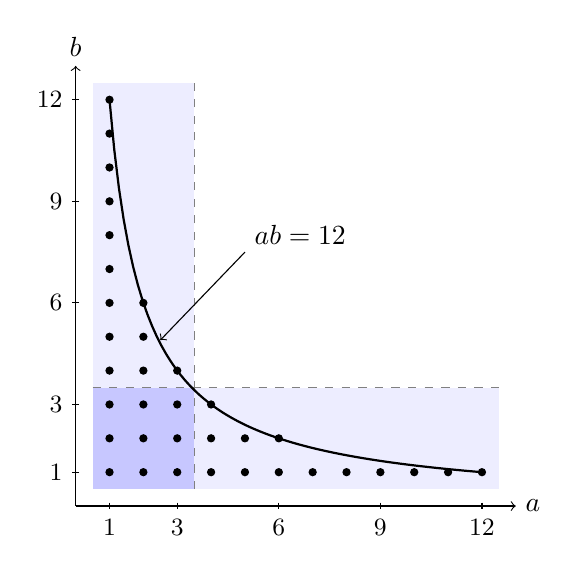
\begin{tikzpicture}[x=0.43cm,y=0.43cm]
 \fill[blue!7] (0.5,0.5) rectangle (3.5,12.5);
 \fill[blue!7] (0.5,0.5) rectangle (12.5,3.5);
 \fill[blue!22] (0.5,0.5) rectangle (3.5,3.5);
 \draw[->] (0,0) -- (13,0) node[right] {\(a\)};
 \draw[->] (0,0) -- (0,13) node[above] {\(b\)};
 \draw[dashed,gray] (3.5,0.5) -- (3.5,12.5);
 \draw[dashed,gray] (0.5,3.5) -- (12.5,3.5);
 \draw[thick,domain=1:12,samples=80] plot (\x,{12/\x});
 \foreach \a in {1,...,12} {
  \foreach \b in {1,...,12} {
   \pgfmathtruncatemacro{\within}{\a*\b<=12}
   \ifnum\within=1\relax
    \fill (\a,\b) circle (1.5pt);
   \fi
  }
 }
 \foreach \t in {1,3,6,9,12} {
  \draw (\t,0.10) -- (\t,-0.10) node[below,font=\small] {\(\t\)};
  \draw (0.10,\t) -- (-0.10,\t) node[left,font=\small] {\(\t\)};
 }
 \node[anchor=west] at (5,8) {\(ab=12\)};
 \draw[->] (5,7.5) -- (2.5,4.9);
\end{tikzpicture}
\caption{双曲线分割：圆点为 \(ab\le12\) 的正整数点。两条浅色带分别选出 \(a\le3\) 与 \(b\le3\) 的整数坐标；深色方块中的九个点需减去一次。}
\label{b3:fig:25-hyperbola}
\end{figure}

这种利用双曲线两侧对称计数的办法称为\term[dirichlet-shuangquxian-fa]{Dirichlet 双曲线法}[Dirichlet hyperbola method]。若直接把 \(\sum_{a\le x}\lfloor x/a\rfloor\) 中每项替成 \(x/a\)，会累积 \(O(x)\) 的取整误差，因而看不见线性次项。以 \(\sqrt x\) 分割以后，只需近似约 \(\sqrt x\) 项，误差便缩小到平方根尺度。若在一个很小的阈值处分割，另一方向仍会留下很长的和；平方根使两个方向的长度保持同一数量级。

部分求和还能把已有的平均值换成新的权重。由刚才的结果，置 \(c=2\gamma-1\)，可写 \(D(t)=t\log t+ct+E(t)\)，其中 \(E(t)=O(\sqrt t)\) 对所有 \(t\ge1\) 成立。取权重 \(1/n\)，得到
\begin{align*}
 \sum_{n\le x}\frac{d(n)}n
 &=\frac{D(x)}x+\int_1^x\frac{D(t)}{t^2}\,\mathrm dt\\
 &=\log x+c+\frac12(\log x)^2+c\log x+O(1)\\
 &=\frac12(\log x)^2+2\gamma\log x+O(1).
\end{align*}
这里端点的误差 \(E(x)/x=O(x^{-1/2})\) 有界，误差积分也一致有界，因为
\[
 \int_1^\infty\frac{|E(t)|}{t^2}\,\mathrm dt
 \le C\int_1^\infty t^{-3/2}\,\mathrm dt<\infty.
\]
一次计数所得的主项与误差，就这样转变成了另一个加权平均值；不需要重新逐项估计 \(d(n)\)。

\subsection{素数计数函数的应用}
\label{b3:subsec:250305}

素数的分布没有简单的逐项公式，但部分求和仍然适用。对实数 \(x\ge2\)，记
\[
 \pi(x)=\#\{p\le x:p\text{ 为素数}\},\qquad
 \vartheta(x)=\sum_{p\le x}\log p.
\]
函数 \(\pi\) 称为\term[sushu-jishu-hanshu]{素数计数函数}[prime-counting function]；函数 \(\vartheta\) 给每个素数加上对数权重。这里的 \(\pi(x)\) 是函数记号，与圆周率 \(\pi\) 应依上下文区分。

在\eqref{b3:eq:25-interval-summation}中取 \(y=2\)，令 \(a_n\) 在素数处为一、其余处为零，并取 \(f(t)=\log t\)。左端不含素数二，故
\[
 \vartheta(x)-\log2
 =\pi(x)\log x-\pi(2)\log2-\int_2^x\frac{\pi(t)}t\,\mathrm dt.
\]
因为 \(\pi(2)=1\)，两个下端项抵消，得到
\begin{equation}\label{b3:eq:25-prime-log-weight}
 \vartheta(x)=\pi(x)\log x-\int_2^x\frac{\pi(t)}t\,\mathrm dt
 \qquad(x\ge2).
\end{equation}
反过来，令 \(a_n\) 在素数处为 \(\log n\)、其余处为零，取 \(f(t)=1/\log t\)。这个权重在 \([2,x]\) 上连续可微，不涉及 \(t=1\) 的奇性。区间公式给
\[
 \pi(x)-1
 =\frac{\vartheta(x)}{\log x}-\frac{\vartheta(2)}{\log2}
       +\int_2^x\frac{\vartheta(t)}{t(\log t)^2}\,\mathrm dt.
\]
利用 \(\vartheta(2)=\log2\)，得到
\begin{equation}\label{b3:eq:25-prime-remove-weight}
 \pi(x)=\frac{\vartheta(x)}{\log x}
       +\int_2^x\frac{\vartheta(t)}{t(\log t)^2}\,\mathrm dt
 \qquad(x\ge2).
\end{equation}
两式在 \(x=2\) 时也成立，此时积分均为零。

\begin{proposition}[素数计数的两种渐近形式]\label{b3:prop:25-prime-counting-equivalence}
对实数 \(x\ge2\)，令 \(\pi(x)=\#\{p\le x:p\text{ 为素数}\}\)、\(\vartheta(x)=\sum_{p\le x}\log p\)。则当 \(x\to\infty\) 时，以下两项等价：
\[
 \vartheta(x)\sim x,\qquad \pi(x)\sim\frac{x}{\log x}.
\]
\end{proposition}
\begin{proof}
先假设 \(\vartheta(x)\sim x\)。这蕴含存在常数 \(C\)，使 \(0\le\vartheta(t)\le Ct\) 对所有 \(t\ge2\) 成立。对 \(x\ge4\)，将\eqref{b3:eq:25-prime-remove-weight}中的积分在 \(\sqrt x\) 处分开：
\begin{align*}
 0\le\int_2^x\frac{\vartheta(t)}{t(\log t)^2}\,\mathrm dt
 &\le C\int_2^{\sqrt x}\frac{\mathrm dt}{(\log t)^2}
       +C\int_{\sqrt x}^x\frac{\mathrm dt}{(\log t)^2}\\
 &\le\frac{C\sqrt x}{(\log2)^2}
       +\frac{4Cx}{(\log x)^2}
 =o\left(\frac x{\log x}\right).
\end{align*}
第一段虽不使用对数衰减，但长度只有 \(\sqrt x\)；第二段长度较大，整个区间上的对数却至少为 \(\frac12\log x\)。因此积分是低阶项，端点项 \(\vartheta(x)/\log x\sim x/\log x\) 给出所求渐近。

反过来，假设 \(\pi(x)\sim x/\log x\)。扩大常数以后，\(0\le\pi(t)\le Ct/\log t\) 对所有 \(t\ge2\) 成立。同样分割可得
\[
 0\le\int_2^x\frac{\pi(t)}t\,\mathrm dt
 \le\frac{C\sqrt x}{\log2}+\frac{2Cx}{\log x}=o(x).
\]
代入\eqref{b3:eq:25-prime-log-weight}，再用 \(\pi(x)\log x\sim x\)，便得到 \(\vartheta(x)\sim x\)。
\end{proof}

这个命题把两种计数的渐近联系起来：建立其中一种以后，Abel 求和便给出另一种。后文由 \(\zeta\) 函数的解析性质研究素数时，对数权重更自然地出现，因此会先估计带权部分和，再用这里的公式还原为素数个数。

% !TeX root = ../../Book3.tex
\section{Dirichlet 级数}
\label{b3:sec:2504}

一般幂级数以圆盘为收敛区域，Dirichlet 级数以右半平面为基本区域。原因是 \(n^{-s}=e^{-s\log n}\)，增大实部会同时压低全部高指标项。

\subsection{收敛横坐标}
\label{b3:subsec:250401}

\begin{definition}\label{b3:def:25-dirichlet-series}
形如 \(D_a(s)=\sum_{n\ge1}a(n)n^{-s}\) 的级数称为\term[dirichlet-jishu]{Dirichlet 级数}[Dirichlet series]。
\end{definition}
若级数在 \(s_0\) 收敛，令 \(b_n=a(n)n^{-s_0}\)。其尾部分和 \(\sum_{M<n\le N}b_n\) 对 \(N\ge M\) 一致趋零。对尾部应用 Abel 求和可知，对任意 \(\operatorname{Re}w>0\)，\(\sum b_nn^{-w}\) 收敛，并在 \(\operatorname{Re}w\ge\delta>0\)、\(|w|\le R\) 一致收敛。因此存在扩展实数 \(\sigma_c\)，使级数在 \(\operatorname{Re}s>\sigma_c\) 收敛且全纯，在 \(\operatorname{Re}s<\sigma_c\) 发散；边界可能随虚部而异。数 \(\sigma_c\) 称为\term[shoulian-hengzuobiao]{收敛横坐标}[abscissa of convergence]。

\subsection{绝对收敛}
\label{b3:subsec:250402}

同样定义\term[juedui-shoulian-hengzuobiao]{绝对收敛横坐标}[abscissa of absolute convergence] \(\sigma_a\)。总有 \(\sigma_c\le\sigma_a\le\sigma_c+1\)，按扩展实数理解。后一个不等式由在 \(s_0\) 收敛推出 \(a(n)n^{-s_0}\) 有界，再与 \(\sum n^{-1-\varepsilon}\) 比较得到。绝对收敛半平面的每个较小闭半平面上有统一主控，因此可以安全乘法和对素数重新分组。

\ProseParagraphBreak

对普通 \(\sum n^{-s}\)，两横坐标都为一；对交错级数，两者分别为零与一。横坐标为零的必要性可由负实部处单项不趋零看出。一个例子同时说明两横坐标可以不同，也说明一般差距上界一能达到。

\subsection{乘法}
\label{b3:subsec:250403}

\begin{proposition}\label{b3:prop:25-product-series}
若 \(D_a,D_b\) 在 \(\operatorname{Re}s=\sigma\) 都绝对收敛，则
\(D_a(s)D_b(s)=D_{a*b}(s)\) 在该直线上成立，且右侧绝对收敛。
\end{proposition}
\begin{proof}
双重绝对和为 \((\sum|a(m)|m^{-\sigma})(\sum|b(n)|n^{-\sigma})<\infty\)。因此可以按积 \(mn=r\) 分组，系数恰为有限和 \(\sum_{m\mid r}a(m)b(r/m)\)。同一个绝对和控制了右侧级数。
\end{proof}
仅仅知道两个级数逐点条件收敛，不能引用这个结论；重新分组的合法性需要另证。

\ProseParagraphBreak

在绝对收敛半平面内部还可逐项求任意次导数。设 \(\sigma_0>\sigma_a\)，再取 \(\delta>0\)。对每个固定整数 \(k\ge0\)，函数 \((\log t)^kt^{-\delta}\) 在 \(t\ge1\) 上有界。因此在 \(\operatorname{Re}s\ge\sigma_0+\delta\) 上，
\[
 \sum_n|a(n)|(\log n)^k n^{-\operatorname{Re}s}
 \le C_{k,\delta}\sum_n|a(n)|n^{-\sigma_0}<\infty.
\]
由一致收敛的导数定理，
\[
 D_a^{(k)}(s)=(-1)^k\sum_{n\ge1}a(n)(\log n)^k n^{-s}.
\]
增加对数权重会影响边界收敛，却不改变右半平面内部的全纯性。这个论证说明为什么下一节可以对 Euler 对数求导，也说明每次求导都应在离边界正距离的紧集上进行估计。

\ProseParagraphBreak

Dirichlet 级数也可视为离散测度的 Laplace 变换：将质量 \(a(n)\) 放在 \(\log n\)，则 \(n^{-s}=e^{-s\log n}\)。相应累积质量为 \(A(e^t)\)。在端点项消失的范围，变量代换 \(x=e^t\) 将部分求和写成
\[
 D_a(s)=s\int_0^\infty A(e^t)e^{-st}\,\mathrm dt.
\]
这项表示把整数上的乘法尺度变为实轴上的加法尺度。若已经知道 \(A(x)\) 的增长，积分容易估计；反过来，只知道变换在某点有极点，通常还不能恢复 \(A(x)\) 的渐近。第二十七章将增加非负性与整条边界的延拓条件，完成那个反向问题。

\subsection{系数卷积}
\label{b3:subsec:250404}

于是 \(D_d=\zeta^2\)、\(D_{\sigma_\alpha}(s)=\zeta(s)\zeta(s-\alpha)\)，最初分别在 \(\operatorname{Re}s>1\) 与 \(\operatorname{Re}s>\max(1,1+\operatorname{Re}\alpha)\) 由绝对收敛证明。\(\mathbf1*\varphi=\operatorname{id}\) 还给 \(D_\varphi(s)=\zeta(s-1)/\zeta(s)\)，但要作除法须先在此处证明分母非零，下一节的 Euler 乘积将提供这一事实。

% !TeX root = ../../Book3.tex
\section{Euler 乘积}
\label{b3:sec:2505}

算术基本定理把整数分解成素数幂，绝对收敛把这个有限分解提升为无穷乘积。对数再把乘法拆成加法，素数幂便成为自然的级数指标。

\subsection{可乘系数的 Euler 乘积}
\label{b3:subsec:250501}

\begin{theorem}[Euler 乘积]\label{b3:thm:25-euler-product}
设 \(a\) 可乘，\(\sum|a(n)|n^{-\sigma}<\infty\)。则
\[
D_a(s)=\prod_p\left(\sum_{r\ge0}a(p^r)p^{-rs}\right),\quad\operatorname{Re}s=\sigma.
\]
若 \(a\) 完全可乘，则各因子为 \((1-a(p)p^{-s})^{-1}\)。
\end{theorem}
\begin{proof}
有限多个素数的局部级数相乘，绝对收敛允许展开，所得系数正是所有仅含这些素因子的整数项。随素数集合扩大，任何固定整数最终纳入，剩余项的绝对和趋零。因此有限乘积趋于 \(D_a\)。完全可乘时局部绝对级数的收敛迫使 \(|a(p)|p^{-\sigma}<1\)，再用几何和公式。
\end{proof}
这一表示称为\term[euler-chengji]{Euler 乘积}[Euler product]。一般可乘函数的某个局部因子可能为零，故不能仅凭“有 Euler 乘积”就宣称函数无零点。几何因子情形还需证明无穷非零因子乘积不坍缩到零。

\subsection{唯一性}
\label{b3:subsec:250502}

\begin{proposition}\label{b3:prop:25-uniqueness}
两个在某个右半平面绝对收敛的 Dirichlet 级数，若代表同一函数，则对应系数相等。
\end{proposition}
\begin{proof}
对差级数，令 \(m\) 为首个非零系数指标。沿实轴 \(s=\sigma\to\infty\)，等式乘以 \(m^\sigma\) 得
\(0=a(m)+\sum_{n>m}a(n)(m/n)^\sigma\)。选绝对收敛点 \(\sigma_0\)，尾项被 \(m^{\sigma_0}|a(n)|n^{-\sigma_0}\) 控制，且逐项趋零。支配收敛得 \(a(m)=0\)，矛盾。
\end{proof}
所以解析乘法等式可以反向识别系数，但须处在确有收敛表示的公共区域。延拓后的函数值本身并不意味着原级数也在那里收敛。

\subsection{Euler 乘积的对数}
\label{b3:subsec:250503}

对 \(a(n)=1\)，\(\sum_p\sum_{r\ge1}|p^{-rs}|/r\) 在 \(\sigma>1\) 局部一致收敛，因为被常数倍的 \(\sum_p p^{-\sigma}\) 控制。于是定义
\[
L(s)=\sum_p\sum_{r\ge1}\frac{p^{-rs}}r,
\quad \zeta(s)=e^{L(s)}.
\]
等式先由有限乘积对数成立，再在局部一致极限中保持。因此 \(\zeta\ne0\) 于 \(\sigma>1\)，并且 \(L\) 是在实轴取实值的全纯对数。无零点性来自这个收敛的指数表示，不能从每个单独因子非零直接推断。

\subsection{对数导数}
\label{b3:subsec:250504}

对紧集 \(\sigma\ge1+\delta\)，导数项的绝对和
\(\sum_{p,r}(\log p)p^{-r\sigma}\) 有界：先求 \(r\) 的几何和，再与 \(\sum_{n\ge2}(\log n)n^{-1-\delta}\) 比较。因此可求导，得到
\begin{equation}\label{b3:eq:25-log-derivative}
-\frac{\zeta'(s)}{\zeta(s)}=\sum_p\sum_{r\ge1}(\log p)p^{-rs}
=\sum_{n\ge1}\frac{\Lambda(n)}{n^s},\quad\operatorname{Re}s>1.
\end{equation}
还可由有限卷积恒等式得到同一结论：\(-\zeta'(s)=D_{\log}(s)\)，而 \(\mathbf1*\Lambda=\log\)，故 \(D_\Lambda\zeta=-\zeta'\)。两条路线分别检验乘积常数与系数权重。

\subsection{对数导数中的 \texorpdfstring{\(\Lambda(n)\)}{\AnalysisPdfCapitalLambda(n)}}
\label{b3:subsec:250505}

对数本身在素数幂 \(p^r\) 处给权重 \(1/r\)；求负导数后乘上 \(r\log p\)，留下 \(\log p\)。这解释了 \(\Lambda\) 为何在所有正次素数幂处取相同值。若只保留素数一次项，所得到的不是 \(-\zeta'/\zeta\)，而会遗漏可估计但不恒零的高次幂项。

\ProseParagraphBreak

作为另一例，\(\sum\mu(n)n^{-s}=\prod_p(1-p^{-s})=1/\zeta(s)\) 在 \(\sigma>1\) 成立。它与卷积逆元 \(\mu*\mathbf1=\varepsilon\) 相符。后面若试图把这一表示向临界带推进，就必须控制 Möbius 部分和；单凭右侧已经延拓不能保证左侧条件收敛。算术抵消与解析延拓之间的区别在素数问题中尤其重要。

\begin{proposition}[平方自由整数与互素整数对的密度]
\label{b3:prop:25-two-densities}
设 \(x\ge2\)。有
\[
 \sum_{n\le x}\mu(n)^2=\frac{x}{\zeta(2)}+O(\sqrt x),
 \qquad
 \sum_{n\le x}\varphi(n)=\frac{x^2}{2\zeta(2)}+O(x\log x).
\]
其中 \(1/\zeta(2)=6/\pi^2\)。
\end{proposition}
\begin{proof}
由平方自由筛选恒等式，先交换有限和，得到
\[
 \sum_{n\le x}\mu(n)^2
 =\sum_{d\le\sqrt x}\mu(d)\left\lfloor\frac{x}{d^2}\right\rfloor
 =x\sum_{d\le\sqrt x}\frac{\mu(d)}{d^2}+O(\sqrt x).
\]
因为 \(|\mu(d)|\le1\)，把最后有限级数延到无穷的误差至多
\(x\sum_{d>\sqrt x}d^{-2}=O(\sqrt x)\)。绝对收敛的 Euler 乘积给无穷和为 \(1/\zeta(2)\)，于是得到第一式。

再令 \(N=\lfloor x\rfloor\)，计数 \(1\le a,b\le N\) 中互素的有序整数对。把 \(\sum_{d\mid\gcd(a,b)}\mu(d)\) 代入其示性函数，得
\[
 C(N)=\sum_{d\le N}\mu(d)\left\lfloor\frac Nd\right\rfloor^2.
\]
对 \(u\ge1\)，有 \(|\lfloor u\rfloor^2-u^2|\le2u\)，所以
\[
 C(N)=N^2\sum_{d\le N}\frac{\mu(d)}{d^2}
          +O\left(N\sum_{d\le N}\frac1d\right)
      =\frac{N^2}{\zeta(2)}+O(N\log N).
\]
对角线上互素的点只有 \((1,1)\)；直线 \(a=b\) 两侧由交换坐标对应。固定较大的坐标 \(n\ge2\)，其下方互素点有 \(\varphi(n)\) 个，故
\(C(N)=1+2\sum_{n=2}^N\varphi(n)=2\sum_{n=1}^N\varphi(n)-1\)。代入并把 \(N^2\) 换成 \(x^2+O(x)\)，得到第二式。\(\zeta(2)\) 的数值由前面已证的正弦乘积或相应留数计算给出。
\end{proof}

同一个常数出现在两种不同计数中，原因都可由素数局部条件解释：平方自由性要求不被 \(p^2\) 整除，互素性要求两个坐标不同时被 \(p\) 整除，两者的局部排除比例均为 \(p^{-2}\)。不过无限多个局部条件的密度不能仅凭直觉相乘。上面的有限反演、取整误差及绝对收敛尾界，才把这种解释变成有效证明。

\ProseParagraphBreak

这些平均计数不需要素数定理。它们使用 \(\sum\mu(d)/d^2\) 的绝对收敛，不要求估计 \(\sum_{d\le x}\mu(d)\) 的相消。相较之下，把 \(1/\zeta(s)\) 的 Dirichlet 级数推进到靠近实部一的边界，需要更精细的算术信息。读者应从所用权重和收敛域判断一个推导实际有多强，而不能只看公式中是否出现 Möbius 函数或素数乘积。


\begin{chaptersummary}
可乘函数由各素数幂处的数据决定；完全可乘函数进一步由各素数处的数据决定。Dirichlet 卷积在每个整数处只有有限项，因而其代数恒等式、逆元和 Möbius 反演都先于解析收敛而成立。进入级数以后，乘法需要双重绝对和，求逆需要足够靠右的收敛域，原来的有限恒等式不能替代这些条件。

Abel 求和把权重的变化与系数部分和分开，既保留抵消，也暴露端点项。它说明为何 \(A(x)=O(x^\alpha)\) 给出 \(\operatorname{Re}s>\alpha\) 的收敛，却不能自动给出边界收敛或绝对收敛。收敛横坐标描述原级数；解析延拓描述与其和函数相接的新表示，两者应始终分清。

Euler 乘积则把唯一素分解用于绝对收敛级数。完全可乘情形的对数可由可和的素数幂级数构造，随后才能安全地取对数导数与商。函数 \(-\zeta'/\zeta\) 的系数 \(\Lambda\) 记录了全部素数幂，下一章将研究 \(\zeta\) 的延拓与零点，第二十七章再把这些解析信息转回素数计数。平方自由整数及互素整数对的密度已经在本章求出，它们只依赖绝对收敛的 Möbius 权重，不需要更深的素数分布估计。
\end{chaptersummary}

\BookExercises

% 题1、3、5、8按本章已证恒等式组织为延伸应用；题2保留原d_3训练并细化误差。
% 题4、6自拟参数例，题7把正文中的发散性升级为有限截断下界。
% 公式校准：NIST DLMF 27.2（Liouville/Jordan定义）及27.4.7（Liouville级数）。
% 未据未取得全文的教材声称具体题号来源；八题均重新组织题面并给完整自证。

\begin{exercise}\label{b3:ex:25-1}
对正整数 \(n=\prod_p p^{\nu_p(n)}\)，记
\[
 \Omega(n)=\sum_p\nu_p(n),\qquad \lambda(n)=(-1)^{\Omega(n)},
 \qquad \Omega(1)=0.
\]
证明 \(\lambda\) 完全可乘，其 Dirichlet 卷积逆元为 \(\mu^2\)，并证明
\[
 \sum_{n\ge1}\frac{\lambda(n)}{n^s}
 =\frac{\zeta(2s)}{\zeta(s)},\qquad \operatorname{Re}s>1.
\]
这里 \(\mu^2(n)\) 指 \(\mu(n)^2\)，不是 \((\mu*\mu)(n)\)。
\end{exercise}
\begin{solution}
每个素数在乘积中的指数相加，故对任意正整数 \(m,n\)，
\[
 \Omega(mn)=\Omega(m)+\Omega(n),\qquad
 \lambda(mn)=\lambda(m)\lambda(n).
\]
不需要互素假设。由\cref{b3:prop:25-completely-inverse}，逆元为逐点乘积 \(\mu(n)\lambda(n)\)。若 \(n\) 含平方素因子，\(\mu(n)=0\)；若 \(n\) 为平方自由整数，则 \(\Omega(n)\) 等于不同素因子的个数，\(\lambda(n)=\mu(n)\)。包括 \(n=1\) 在内，均有 \(\mu(n)\lambda(n)=\mu(n)^2\)。

因为 \(|\lambda(n)|=1\)，其级数在 \(\operatorname{Re}s>1\) 绝对收敛。在这个范围内应用 Euler 乘积，并在各素数处使用几何恒等式，得
\[
 \sum_{n\ge1}\frac{\lambda(n)}{n^s}
 =\prod_p(1+p^{-s})^{-1}
 =\prod_p\frac{1-p^{-s}}{1-p^{-2s}}
 =\frac{\zeta(2s)}{\zeta(s)}.
\]
最后一步可先对有限乘积取商，再取极限；两个 \(\zeta\) 因子的参数实部均大于一，分母非零。此公式没有断言原级数在实部不超过一时如何收敛。
\end{solution}

\begin{exercise}\label{b3:ex:25-2}
令 \(d_3(n)\) 为满足 \(abc=n\) 的有序正整数三元组 \((a,b,c)\) 的个数。设 \(\gamma\) 为 Euler 常数，证明当实数 \(x\to\infty\) 时，
\[
 \sum_{n\le x}d_3(n)
 =\frac12x(\log x)^2+(3\gamma-1)x\log x+O(x).
\]
\end{exercise}
\begin{solution}
记 \(D(y)=\sum_{n\le y}d(n)\)。由\cref{b3:prop:25-divisor-average}，扩大误差常数后可对所有 \(y\ge1\) 写成
\[
 D(y)=y\log y+(2\gamma-1)y+O(\sqrt y).
\]
固定三元组的第一个因子 \(a\)，其余两个因子的乘积不超过 \(x/a\)，所以
\[
 \begin{aligned}
 \sum_{n\le x}d_3(n)
 &=\sum_{a\le x}D(x/a)\\
 &=x\log x\sum_{a\le x}\frac1a
   -x\sum_{a\le x}\frac{\log a}{a}
   +(2\gamma-1)x\sum_{a\le x}\frac1a
   +O\left(\sqrt x\sum_{a\le x}a^{-1/2}\right).
 \end{aligned}
\]
积分比较给 \(\sum_{a\le x}a^{-1/2}=O(\sqrt x)\)，故最后误差为 \(O(x)\)。

令 \(N=\lfloor x\rfloor\)。由调和和估计及 \(\log N=\log x+O(1/x)\)，有
\[
 \sum_{a\le x}\frac1a=\log x+\gamma+O(1/x).
\]
另一个加权和满足
\[
 \sum_{a\le x}\frac{\log a}{a}
 =\frac12(\log x)^2+O(1).
\]
为看清误差，注意 \(f(t)=\log t/t\) 在 \(t\ge e\) 上非负递减；在相邻整数区间比较 \(f\) 的上、下矩形和，离散和与积分之差被一个固定常数控制。开头有限项以及 \(N\) 到 \(x\) 的积分也有界，而 \(\int_1^x(\log t)/t\,\mathrm dt=\tfrac12(\log x)^2\)。

代入后，\(x(\log x)^2\) 的系数为 \(1-\tfrac12=\tfrac12\)；\(x\log x\) 的系数为 \(\gamma+(2\gamma-1)=3\gamma-1\)。其余项均为 \(O(x)\)，结论得证。这里三元组有序，无须除以任何排列数。
\end{solution}

\begin{exercise}\label{b3:ex:25-3}
固定整数 \(k\ge2\)，定义
\[
 J_k(n)=\#\{(a_1,\ldots,a_k)\in\{1,\ldots,n\}^k:
                 \gcd(a_1,\ldots,a_k,n)=1\}.
\]
证明
\[
 J_k(n)=n^k\prod_{p\mid n}(1-p^{-k}),\qquad
 \sum_{n\ge1}\frac{J_k(n)}{n^s}
 =\frac{\zeta(s-k)}{\zeta(s)}
 \quad(\operatorname{Re}s>k+1),
\]
并求出平均值
\[
 \sum_{n\le x}J_k(n)
 =\frac{x^{k+1}}{(k+1)\zeta(k+1)}+O_k(x^k)
 \qquad(x\to\infty).
\]
\end{exercise}
\begin{solution}
把 Möbius 约数和用于全部坐标与 \(n\) 的最大公因数。若 \(d\mid n\)，每个坐标中可被 \(d\) 整除的数有 \(n/d\) 个，因此
\[
 J_k(n)=\sum_{d\mid n}\mu(d)(n/d)^k
       =n^k\sum_{d\mid n}\frac{\mu(d)}{d^k}
       =n^k\prod_{p\mid n}(1-p^{-k}).
\]
最后一步只展开一个有限乘积，\(n=1\) 时空乘积为一。第一式也说明 \(J_k=\mu*\operatorname{id}_k\)。当 \(\operatorname{Re}s>k+1\) 时，两个因子级数绝对收敛；卷积乘法与\eqref{b3:eq:25-mobius-series}便给出所求商式。直接上界 \(J_k(n)\le n^k\) 也保证左侧绝对收敛。

为求平均值，再交换有限和：
\[
 \sum_{n\le x}J_k(n)
 =\sum_{d\le x}\mu(d)\sum_{m\le x/d}m^k.
\]
正函数 \(t^k\) 单调递增，矩形和与积分比较给出，对全部实数 \(Y\ge1\)，
\[
 \sum_{m\le Y}m^k=\frac{Y^{k+1}}{k+1}+O_k(Y^k).
\]
先在整数上以相邻上下积分夹住该和，再将 \(\lfloor Y\rfloor\) 换成 \(Y\)，所付出的误差仍为 \(O_k(Y^k)\)。于是
\[
 \sum_{n\le x}J_k(n)
 =\frac{x^{k+1}}{k+1}\sum_{d\le x}\frac{\mu(d)}{d^{k+1}}
  +O_k\left(x^k\sum_{d\le x}d^{-k}\right).
\]
由于 \(k\ge2\)，误差中的和一致有界。主项的级数延长到无穷时，误差至多为常数倍
\(x^{k+1}\sum_{d>x}d^{-k-1}=O_k(x)\)，也被 \(O_k(x^k)\) 包含。无穷和为 \(1/\zeta(k+1)\)，得到结论。若取 \(k=1\)，同一方法中的误差和成为调和和，通常只能给 \(O(x\log x)\)；这说明题目为何单列 \(k\ge2\)。
\end{solution}

\begin{exercise}\label{b3:ex:25-4}
设 \(\alpha\in\mathbb R\)，令 \(a(2^j)=2^{j\alpha}/j\)（\(j\ge1\)），其余正整数处 \(a(n)=0\)。求 Dirichlet 级数 \(D_a(s)=\sum_{n\ge1}a(n)n^{-s}\) 的两个收敛横坐标，并逐点判定边界 \(s=\alpha+\mathrm it\) 上的收敛性。
\end{exercise}
\begin{solution}
按自然顺序求和与按二的正次幂求和给出同一极限，所以
\[
 D_a(s)=\sum_{j\ge1}\frac{(2^{\alpha-s})^j}{j}.
\]
若 \(\operatorname{Re}s>\alpha\)，括号内的模小于一，级数绝对收敛；若 \(\operatorname{Re}s<\alpha\)，非零项的模为 \(2^{j(\alpha-\operatorname{Re}s)}/j\)，不趋于零。因此 \(\sigma_c=\sigma_a=\alpha\)。

在边界上，记 \(z=e^{-\mathrm it\log2}\)，于是 \(|z|=1\)。若 \(t\log2\in2\pi\mathbb Z\)，则 \(z=1\)，级数成为发散的调和级数。若 \(z\ne1\)，则
\[
 \left|\sum_{j=1}^N z^j\right|
 =\left|\frac{z(1-z^N)}{1-z}\right|
 \le\frac2{|1-z|}.
\]
以 \(1/j\) 为权重作 Abel 求和，或应用\cref{b3:prop:25-partial-sum-convergence}于指标 \(j\)，便知 \(\sum z^j/j\) 收敛。边界上的绝对级数始终为 \(\sum1/j\)，故所有非共振点均为条件收敛点。相同的两个横坐标并不能说明整条边界线的收敛行为一致。
\end{solution}

\begin{exercise}\label{b3:ex:25-5}
设 \(d(n)\) 为正整数 \(n\) 的正约数个数。证明
\[
 \sum_{n\ge1}\frac{d(n)^2}{n^s}
 =\frac{\zeta(s)^4}{\zeta(2s)},\qquad\operatorname{Re}s>1.
\]
解释为什么左侧不能直接由 \(D_d(s)^2\) 得到。
\end{exercise}
\begin{solution}
先检查绝对收敛。固定 \(\sigma=\operatorname{Re}s>1\)，在\cref{b3:prop:25-divisor-small-power}中取 \(\epsilon=(\sigma-1)/4\)，有 \(d(n)\le C_\epsilon n^\epsilon\)。故
\[
 d(n)^2n^{-\sigma}\le C_\epsilon^2 n^{-(\sigma+1)/2},
\]
右边可和。逐点平方 \(d^2\) 仍可乘，而 \(d(p^r)^2=(r+1)^2\)。

在 \(|X|<1\) 内，几何级数可逐项求导。对 \(\sum_{r\ge0}(r+1)X^r=(1-X)^{-2}\) 再施以算子 \(X\,d/dX+1\)，得到
\[
 \sum_{r\ge0}(r+1)^2X^r
 =\frac{2X}{(1-X)^3}+\frac1{(1-X)^2}
 =\frac{1+X}{(1-X)^3}
 =\frac{1-X^2}{(1-X)^4}.
\]
因此 Euler 乘积给
\[
 D_{d^2}(s)=\prod_p\frac{1-p^{-2s}}{(1-p^{-s})^4}
          =\frac{\zeta(s)^4}{\zeta(2s)}.
\]
取商时 \(\operatorname{Re}(2s)>2\)，分母确实非零。

另一方面，\(D_d^2=D_{d*d}=\zeta^4\)，其系数是四重因子计数 \(d_4\)，而非逐点平方。例如在 \(p^2\) 处，\(d(p^2)^2=9\)，但
\[
 (d*d)(p^2)=d(1)d(p^2)+d(p)d(p)+d(p^2)d(1)=10.
\]
这给出了两种乘法不同的具体检查。
\end{solution}

\begin{exercise}\label{b3:ex:25-6}
设整数 \(m\ge2\)，\(\omega=e^{2\pi\mathrm i/m}\)。求 \(\sum_{n\ge1}\omega^n n^{-s}\) 的两个收敛横坐标，并证明
\[
 \sum_{n\ge1}\frac{\omega^n}{n}
 =-\log\bigl(2\sin(\pi/m)\bigr)
   +\mathrm i\left(\frac\pi2-\frac\pi m\right).
\]
右侧的 \(\log\) 是正实数的实对数。
\end{exercise}
\begin{solution}
有限几何和给
\[
 \left|\sum_{n=1}^N\omega^n\right|\le\frac2{|1-\omega|}.
\]
部分求和遂保证实部大于零时收敛；实部不大于零时，原级数的各项模不趋于零。所以 \(\sigma_c=0\)。由于 \(|\omega^n|=1\)，绝对级数为 \(\sum n^{-\sigma}\)，故 \(\sigma_a=1\)。

为了计算边界于圆盘的幂级数值，先令 \(0\le r<1\)。在单位圆盘内积分几何级数，得
\[
 \sum_{n\ge1}\frac{(r\omega)^n}{n}=-\operatorname{Log}(1-r\omega),
\]
其中 \(\operatorname{Log}\) 取右半平面上的全纯分支，并在正实轴上等于实对数；因为
\(\operatorname{Re}(1-r\omega)>0\)，它沿此路径始终有定义。

还须证明左侧在 \(r\uparrow1\) 时趋于题目中的收敛和。对于任意尾段，\(\omega^n\) 的部分和有统一界 \(C=2/|1-\omega|\)。权重 \(r^n/n\) 对 \(n\) 非负递减，有限 Abel 求和因此给
\[
 \left|\sum_{n=N+1}^{M}\frac{r^n\omega^n}{n}\right|
 \le \frac{C}{N+1}\qquad(0\le r\le1,\ M>N).
\]
固定 \(r\) 后令 \(M\to\infty\)，此界仍成立，并且不依赖 \(r\)。先把 \(N\) 选大以控制所有尾部，再在前 \(N\) 项令 \(r\uparrow1\)，就得到所需的极限交换。

最后，
\[
 1-\omega=2\sin(\pi/m)
       \exp\left(\mathrm i\left(\frac\pi m-\frac\pi2\right)\right).
\]
这里 \(\sin(\pi/m)>0\)，辐角 \(\pi/m-\pi/2\) 落在 \((-\pi/2,0]\) 内，和已选分支一致。代入 \(-\operatorname{Log}(1-\omega)\) 即得公式。\(m=2\) 时退化为 \(\sum(-1)^n/n=-\log2\)，也核对了符号。
\end{solution}

\begin{exercise}\label{b3:ex:25-7}
证明对每个整数 \(N\ge2\)，有有限截断下界
\[
 \sum_{p\le N}\frac1p\ge\log\log(N+1)-1.
\]
证明中不得将只在 \(\operatorname{Re}s>1\) 建立的无穷 Euler 乘积直接代入 \(s=1\)。
\end{exercise}
\begin{solution}
只对有限多个素数取乘积，并把每个几何因子展开：
\[
 P_N=\prod_{p\le N}(1-p^{-1})^{-1}
 =\sum_{\substack{n\ge1\\p\mid n\Rightarrow p\le N}}\frac1n.
\]
这是有限多个绝对收敛几何级数的乘法，所以在此处没有无穷素数乘积问题。每个 \(1\le n\le N\) 的素因子都不超过 \(N\)，故
\[
 P_N\ge H_N\ge\int_1^{N+1}\frac{dt}{t}=\log(N+1).
\]
另一方面，对这个有限乘积取实对数，有
\[
 \log P_N
 =\sum_{p\le N}\frac1p
  +\sum_{p\le N}\sum_{r\ge2}\frac1{r p^r}.
\]
后面的双重和非负，且不超过
\[
 \sum_{n\ge2}\sum_{r\ge2}n^{-r}
 =\sum_{n\ge2}\frac1{n(n-1)}=1.
\]
把两边的上下界合并，得到
\(\log\log(N+1)\le\log P_N\le\sum_{p\le N}p^{-1}+1\)，即为结论。
\end{solution}

\begin{exercise}\label{b3:ex:25-8}
对整数 \(n\ge1\)，令
\[
 r_j(n)=\#\{(x_1,\ldots,x_j)\in\mathbb Z^j:
                   x_1^2+\cdots+x_j^2=n\},\qquad j=2,4.
\]
令 \(\chi_4(d)\) 在偶数处为零，在模四余一、余三处分别为一、负一，并记 \(L_4(s)=\sum_{n\ge1}\chi_4(n)n^{-s}\)。使用\cref{b3:thm:24-two-squares,b3:thm:24-four-squares}的除数公式，证明
\begin{align*}
 \sum_{n\ge1}\frac{r_2(n)}{n^s}
 &=4\zeta(s)L_4(s),&&\operatorname{Re}s>1,\\
 \sum_{n\ge1}\frac{r_4(n)}{n^s}
 &=8(1-4^{1-s})\zeta(s)\zeta(s-1),&&\operatorname{Re}s>2.
\end{align*}
再说明第二个和函数可亚纯延拓到 \(s=2\) 的一个邻域，且在那里有留数为 \(\pi^2\) 的单极点。
\end{exercise}
\begin{solution}
前章中的计数保留坐标次序和正负号，其公式为
\[
 r_2(n)=4\sum_{d\mid n}\chi_4(d),\qquad
 r_4(n)=8\sum_{\substack{d\mid n\\4\nmid d}}d.
\]
第一式即 \(r_2=4(\mathbf1*\chi_4)\)。由于 \(|\chi_4(d)|\le1\)，\(\mathbf1\) 和 \(\chi_4\) 的级数都在实部大于一时绝对收敛，卷积乘法给出第一个所求等式，并同时保证左侧绝对收敛。

对第二式，设 \(b(d)=d\) 当 \(4\nmid d\)，而 \(b(d)=0\) 当 \(4\mid d\)。于是 \(r_4=8(\mathbf1*b)\)，且在实部大于二时，
\[
 \begin{aligned}
 D_b(s)
 &=\sum_{d\ge1}d^{1-s}-\sum_{m\ge1}(4m)^{1-s}\\
 &=(1-4^{1-s})\zeta(s-1).
 \end{aligned}
\]
这些级数都绝对收敛，因此乘以 \(\zeta(s)\) 给出第二式。原计数还满足 \(r_j(0)=1\)，但题目级数从 \(n=1\) 起，零指标不能放入 \(n^{-s}\)，也没有贡献额外常数项。

由\eqref{b3:eq:25-zeta-integral}，\(\zeta(u)\) 在 \(u=1\) 附近有留数为一的单极点。因此 \(\zeta(s-1)\) 在 \(s=2\) 附近有同样的留数；\(\zeta(s)\) 在二附近则由绝对收敛级数定义为全纯函数。右侧便给出所求延拓，留数为
\[
 8(1-4^{-1})\zeta(2)=6\cdot\frac{\pi^2}{6}=\pi^2.
\]
这个数也与\cref{b3:prop:24-four-square-average}中的累计主项
\(\sum_{n\le x}r_4(n)\sim(\pi^2/2)x^2\) 相呼应：若在部分求和积分中单看主项，所得奇部为
\[
 s\int_1^\infty\frac{\pi^2}{2}t^2t^{-s-1}\,\mathrm dt
 =\frac{\pi^2s}{2(s-2)},
\]
其在二的留数正好是 \(\pi^2\)。这一比较解释常数关系；上面证明延拓和留数时，依据的是已得到的精确乘积公式。
\end{solution}

% !TeX root = ../../Book3.tex
\chapter{Riemann \texorpdfstring{\(\zeta\)}{\AnalysisPdfZeta} 函数}
\label{b3:ch:26}
\BookChapterNumber{b3:ch:26}
% 本章摘要（不计入编号）
\begin{chapterabstract}
Riemann zeta 函数最初由整数的 Dirichlet 级数定义，却通过 theta 的 Mellin 变换获得全平面延拓。本章证明其唯一极点、函数方程与平凡零点，明确尚待下一章处理的边界无零点问题；末节将非平凡零点编码在阶一整函数 \(\xi\) 的典范乘积中。
\end{chapterabstract}

% 本章目标（不计入编号）
\begin{learninggoals}
能够重建 theta 积分的分割与换元，核对 Gamma 因子和极点留数；区分原级数、延拓函数与完备函数的定义域；能准确说明零点对称性、已证零点范围及 Riemann 猜想的内容。
\end{learninggoals}

素数由 Euler 乘积进入 \(\zeta\)，全平面对称却来自高斯求和。把两个表达式连接起来，需要先给它们共同的 Mellin 积分，再把原点的两个显式奇性扣除。所需工具为\chapref{b3:ch:21}、\chapref{b3:ch:24}和\chapref{b3:ch:25}，末节另用 Hadamard 分解。Edwards 的《Riemann's Zeta Function》\cite{Edwards2001Riemann}可供继续阅读零点与显式公式的联系。

% !TeX root = ../../Book3.tex
\section{Dirichlet 级数与 Euler 乘积}
\label{b3:sec:2601}

本章把上一章的收敛级数扩展为全平面的亚纯函数。首先保留它与素数的直接关系；随后用高斯的参数反演得到在原级数收敛域之外仍有意义的表达式。

\subsection{在 \texorpdfstring{\(\operatorname{Re}s>1\)}{Re(s)>1} 上的收敛性}
\label{b3:subsec:260101}

\begin{definition}\label{b3:def:26-zeta}
在 \(\operatorname{Re}s>1\) 上定义\term[riemann-zeta-hanshu]{Riemann zeta 函数}[Riemann zeta function]
\(\zeta(s)\coloneqq\sum_{n\ge1}n^{-s}\)。
\end{definition}
\symidx{\(\zeta(s)\)：Riemann zeta 函数}
对紧集 \(\operatorname{Re}s\ge1+\delta\)，由 \(\sum n^{-1-\delta}<\infty\) 得局部一致绝对收敛，故全纯；任意固定次导数可逐项计算，因为 \((\log n)^k\) 被小幂 \(n^{\delta/2}\) 控制。在正实轴，\(\zeta(\sigma)>1\)，且 \(\zeta(\sigma)\to1\) 当 \(\sigma\to\infty\)。

\subsection{Euler 乘积}
\label{b3:subsec:260102}

\cref{b3:thm:25-euler-product}给 \(\zeta(s)=\prod_p(1-p^{-s})^{-1}\)。更强的是前章已经建立收敛全纯对数
\(\log\zeta(s)=\sum_{p,r\ge1}p^{-rs}/r\)，从而在这个半平面无零点。若把乘积形式延伸到 \(\operatorname{Re}s\le1\)，它通常不再收敛；后面的解析延拓不能被称为该无穷乘积在原意义下的值。

\ProseParagraphBreak

绝对收敛还给出不依赖虚部的上下界。由原级数及 Möbius 逆级数，
\[
 |\zeta(\sigma+\mathrm it)|\le\zeta(\sigma),\qquad
 \left|\frac1{\zeta(\sigma+\mathrm it)}\right|
 \le\sum_{n\ge1}\frac{|\mu(n)|}{n^\sigma}\le\zeta(\sigma),
 \quad\sigma>1.
\]
所以在每条固定的直线 \(\sigma>1\) 上，函数既有上界，也与零保持正距离。不过当 \(\sigma\downarrow1\) 时，这个下界趋于零，因而不能排除边界零点。无零点区域是否能够扩大，必须从新的信息判断。

\subsection{素数与 \texorpdfstring{\(\zeta\)}{\AnalysisPdfZeta} 函数}
\label{b3:subsec:260103}

\(\zeta\) 将所有整数编码，而其对数只在素数幂上有系数。沿实轴 \(\sigma\downarrow1\)，\(\zeta(\sigma)\) 的发散迫使素数无限多，也迫使 \(\sum_p1/p\) 发散。这类结论仍比素数定理弱：它们不能确定 \(\pi(x)\) 的渐近常数，后者需要控制函数在边界直线上的零点。

% !TeX root = ../../Book3.tex
\section{Mellin 变换与 \texorpdfstring{\(\theta\)}{\AnalysisPdfTheta} 函数}
\label{b3:sec:2602}

Gamma 因子出现的原因不是人为修饰：对一个高斯项做 Mellin 积分，二次尺度自然把参数变为 \(s/2\)，并产生 \(\pi^{-s/2}\Gamma(s/2)\)。

\subsection{Mellin 变换}
\label{b3:subsec:260201}

记 \(\vartheta(t)=\sum_{n\in\mathbb Z}e^{-\pi n^2t}\)、\(h(t)=(\vartheta(t)-1)/2=\sum_{n\ge1}e^{-\pi n^2t}\)，\(t>0\)。对 \(\sigma>1\) 可用 Tonelli 估计绝对值并换序：
\[
\int_0^\infty h(t)t^{s/2-1}\,\mathrm{d}t
=\sum_{n\ge1}(\pi n^2)^{-s/2}\Gamma(s/2)
=\pi^{-s/2}\Gamma(s/2)\zeta(s).
\]
绝对积分为 \(\pi^{-\sigma/2}\Gamma(\sigma/2)\zeta(\sigma)<\infty\)，所以复参数换序并非仅由每一项可积推出。

\subsection{Gamma 函数}
\label{b3:subsec:260202}

Gamma 函数的无零点性使这个乘法不会在右半平面创造新零点。其极点以后却会抵消 \(\zeta\) 的负偶数零点，所以除去 Gamma 因子时必须单独查看局部阶数。特别是 \(s=0\)，Gamma 有极点而 \(\zeta\) 最终并不为零，不能把所有 Gamma 极点一概称为平凡零点的位置。

\subsection{\texorpdfstring{\(\theta\)}{\AnalysisPdfTheta} 函数}
\label{b3:subsec:260203}

由\secref{b3:sec:2401}的高斯求和，\(\vartheta(t)=t^{-1/2}\vartheta(1/t)\)。于是
\[
h(t)=t^{-1/2}h(1/t)+\frac12(t^{-1/2}-1).
\]
这是延拓的关键等式：右侧第一项在 \(t\downarrow0\) 时带指数小因子，另外两项完整记录原点的幂次奇性。只减去常数一还不能使原点积分对所有参数收敛；还必须处理 \(t^{-1/2}\) 项。

\subsection{热核观点}
\label{b3:subsec:260204}

函数 \(\vartheta(t)\) 也可视为圆周高斯热核在原点的值，\(n^2\) 对应离散频率的平方。减去一是在去掉零频率。小时间的 \(t^{-1/2}\) 主项反映一维局部尺度；Mellin 积分把这个幂次转成 \(s=1\) 的极点。这个解释无需将谱语言当作证明，全部常数已由高斯换元确定。

\ProseParagraphBreak

为了使热核的归一化完全明确，在周期一的圆周上取 Fourier 模态 \(e^{2\pi\mathrm inx}\)。算子 \(-\partial_x^2\) 的对应特征值为 \(4\pi^2n^2\)，故热核在时间 \(\tau\) 的对角值是
\[
 K_\tau(0)=\sum_{n\in\mathbb Z}e^{-4\pi^2n^2\tau}
          =\vartheta(4\pi\tau).
\]
令 \(t=4\pi\tau\)，才得到前面使用的 \(\vartheta(t)\)。时间参数若不同时缩放，会使 Mellin 变换中的 \(\pi\) 因子发生变化。对角热核的大小与变换公式都可以从 Fourier 级数逐项验证，无需额外假定抽象谱定理。

\ProseParagraphBreak

小时间的余项也有直接界。对 \(u\ge1\)，利用 \(n^2\ge1+3(n-1)\) 可得
\[
 0<h(u)\le\frac{e^{-\pi u}}{1-e^{-3\pi u}}
          \le\frac{e^{-\pi u}}{1-e^{-3\pi}}.
\]
代入参数反演，便有
\[
 \vartheta(t)=t^{-1/2}
       +O\bigl(t^{-1/2}e^{-\pi/t}\bigr),\qquad0<t\le1.
\]
这比仅说余项趋于零强得多。对任意固定的复参数紧集，指数小量乘上 \(t\) 的任意固定负幂仍可积；因此扣去主项后能够穿过任意有限条竖直线。下一节的全平面延拓正是把这一估计写成一条统一的积分公式。

% !TeX root = ../../Book3.tex
\section{解析延拓}
\label{b3:sec:2603}

延拓的困难集中在积分的端点，而不在每个固定正实数处的被积函数。这里给出两条路线：Euler--Maclaurin 方法逐步减去端点主项，适合得到截断公式和误差；theta 方法利用反演，将两个端点合成一个指数收敛积分，同时显露 \(s\) 与 \(1-s\) 的对称性。希望得到具体截断误差时，可以选读第一小节的 Euler--Maclaurin 方法。

\OptionalSubsection{Euler–Maclaurin 方法}{b3:subsec:260301}

\eqref{b3:eq:25-zeta-integral}已在 \(\operatorname{Re}s>1\) 给出
\[
 \zeta(s)=\frac{s}{s-1}
      -s\int_1^\infty\{t\}t^{-s-1}\,\mathrm dt.
\]
因为 \(0\le\{t\}<1\)，右侧积分在 \(\operatorname{Re}s>0\) 仍绝对收敛。要继续向左，就不能只估计分数部分的大小，还要利用它减去平均值以后每个周期的积分为零。一个均值为零的周期函数有有界周期原函数；分部积分把这个原函数留下，同时让权重多衰减一个 \(t^{-1}\)。反复实行这一操作，得到\term[euler-maclaurin-qiuhe-gongshi]{Euler--Maclaurin 求和公式}[Euler--Maclaurin summation formula]。

\ProseParagraphBreak

为使每次积分中的常数唯一确定，先定义\term[bernoulli-duoxiangshi]{Bernoulli 多项式}[Bernoulli polynomial]。置 \(B_0(x)=1\)；对整数 \(j\ge1\)，以
\[
 B_j'(x)=jB_{j-1}(x),
 \quad \int_0^1B_j(x)\,\mathrm dx=0
\]
唯一确定多项式 \(B_j\)。导数条件留下一个常数，零平均条件恰好确定它。前几项为
\[
 \begin{aligned}
 B_1(x)&=x-\frac12,\quad
 B_2(x)=x^2-x+\frac16,\\
 B_3(x)&=x^3-\frac32x^2+\frac12x,\\
 B_4(x)&=x^4-2x^3+x^2-\frac1{30}.
 \end{aligned}
\]
数 \(B_j\coloneqq B_j(0)\) 称为\term[bernoulli-shu]{Bernoulli 数}[Bernoulli number]。省略自变量的 \(B_j\) 是常数，带自变量的 \(B_j(x)\) 是多项式；例如 \(B_1=-1/2\)、\(B_2=1/6\)、\(B_4=-1/30\)。这里固定了 \(B_1\) 的负号约定。

\ProseParagraphBreak

记 \(\widetilde B_j(t)=B_j(\{t\})\)。这些函数有界且一周期；对 \(j\ge2\)，它们在整数点也是连续的，因为
\[
 B_j(1)-B_j(0)=j\int_0^1B_{j-1}(x)\,\mathrm dx=0.
\]
此外，递推中的导数与零平均条件给出反射关系
\[
 B_j(1-x)=(-1)^jB_j(x).
\]
具体地，若此式对 \(j-1\) 成立，则 \((-1)^jB_j(1-x)\) 与 \(B_j(x)\) 有相同导数和相同的零积分；它们的差为积分也为零的常数，故相等。\(j=0\) 提供归纳起点。结合整数端点相等性可知，奇数 \(j\ge3\) 时两端值既相等又互为相反数，因而均为零。这正是截断公式只留下偶数 Bernoulli 项的原因。

\begin{proposition}[Euler--Maclaurin 截断公式]\label{b3:prop:26-euler-maclaurin}
设 \(N,m\ge1\) 为整数，Bernoulli 多项式由 \(B_0(x)=1\)、\(B_j'=jB_{j-1}\) 及 \(\int_0^1B_j=0\)（\(j\ge1\)）确定，记 \(B_j=B_j(0)\)、\(\widetilde B_j(t)=B_j(\{t\})\)，并令
\[
 (s)_0=1,\quad (s)_j=s(s+1)\cdots(s+j-1)\quad(j\ge1).
\]
原在 \(\operatorname{Re}s>1\) 由 \(\sum_{n\ge1}n^{-s}\) 定义的 \(\zeta\) 有亚纯延拓到 \(\operatorname{Re}s>1-2m\)，且在该半平面有
\begin{equation}\label{b3:eq:26-euler-maclaurin}
 \begin{aligned}
 \zeta(s)={}&\sum_{n<N}n^{-s}+\frac{N^{1-s}}{s-1}+\frac{N^{-s}}2\\
 &+\sum_{r=1}^m\frac{B_{2r}}{(2r)!}
       (s)_{2r-1}N^{1-s-2r}+R_m(s,N),
 \end{aligned}
\end{equation}
其中正实数的复幂用实对数定义，\(s=1\) 处按亚纯函数解释，并且
\[
 R_m(s,N)=-\frac{(s)_{2m}}{(2m)!}
       \int_N^\infty\widetilde B_{2m}(t)t^{-s-2m}\,\mathrm dt.
\]
余项在所述半平面全纯；若 \(\sigma=\operatorname{Re}s>1-2m\)，则
\begin{equation}\label{b3:eq:26-euler-maclaurin-bound}
 |R_m(s,N)|\le
 \frac{|(s)_{2m}|}{(2m)!}\cdot
 \frac{\|B_{2m}\|_{L^\infty(0,1)}}{\sigma+2m-1}
 N^{1-\sigma-2m}.
\end{equation}
不同 \(m,N\) 所得的延拓在共同定义域上一致。
\end{proposition}
\begin{proof}
首先限制 \(\sigma>1\)，保证最初的无穷求和与各个端点极限合法。由\cref{b3:prop:25-integral-summation}，对整数 \(N\) 后面的尾项有
\[
 \sum_{n>N}n^{-s}
 =-N^{1-s}+s\int_N^\infty\lfloor t\rfloor t^{-s-1}\,\mathrm dt.
\]
加入 \(N^{-s}\)，再代入 \(\lfloor t\rfloor=t-1/2-\widetilde B_1(t)\)，计算前两项幂积分，得到
\[
 \sum_{n\ge N}n^{-s}
 =\frac{N^{1-s}}{s-1}+\frac12N^{-s}
       -s\int_N^\infty\widetilde B_1(t)t^{-s-1}\,\mathrm dt.
\]
虽然 \(\widetilde B_1\) 在整数点跳跃，但它在每个开单位区间内为 \(\widetilde B_2/2\) 的导数。逐区间分部积分时，\(B_2(1)=B_2(0)\) 使内部端点相消；其在无穷端的有界性与权重衰减使该端点消失。下端点给出
\[
 -s\int_N^\infty\widetilde B_1(t)t^{-s-1}\,\mathrm dt
 =\frac{B_2}{2!}sN^{-s-1}
       -\frac{(s)_2}{2!}\int_N^\infty
                     \widetilde B_2(t)t^{-s-2}\,\mathrm dt.
\]
这是 \(m=1\) 的公式，也核定了余项前的负号。

假设已经得到偶数阶 \(2r\) 的余项。再分部积分时，原函数为 \(\widetilde B_{2r+1}/(2r+1)\)，其两个整数端点都为零，因此没有新的边界贡献；随后使用 \(\widetilde B_{2r+2}/(2r+2)\) 再分部积分，下端点恰给下一项
\[
 \frac{B_{2r+2}}{(2r+2)!}(s)_{2r+1}N^{-s-2r-1}.
\]
余项仍有负号，阶数变为 \(2r+2\)。内部整数端点依靠相邻两端值相等而相消。在 \(\sigma>1\) 中所有无穷端点均为零，故归纳得到所述有限展开。

最后利用 \(\widetilde B_{2m}\) 有界，对 \(\sigma>1-2m\) 计算
\[
 \int_N^\infty t^{-\sigma-2m}\,\mathrm dt
 =\frac{N^{1-\sigma-2m}}{\sigma+2m-1}.
\]
这证明余项界。在该半平面任一紧集上，指数离临界值有正距离；参数微分增加的 \(\log t\) 幂仍可积。因此余项全纯，右端只可能在一处有极点，并在原半平面与原级数相同，故给出延拓。任意两种截断表达式均在 \(\sigma>1\) 相同，恒等定理保证它们在连通的共同半平面相同。
\end{proof}

一个实际计算应同时报告近似值和误差。取 \(m=1\)，因为 \(B_2(x)=x^2-x+1/6\) 在 \([0,1]\) 上的最大绝对值为 \(1/6\)，有
\[
 |R_1(s,N)|\le
   \frac{|s(s+1)|}{12(\sigma+1)}N^{-\sigma-1},
 \quad \sigma>-1.
\]
例如 \(s=2\)、\(N=10\) 时，
\[
 \left|\zeta(2)-
   \left(\sum_{n=1}^{9}\frac1{n^2}+\frac1{10}
                   +\frac1{200}+\frac1{6000}\right)\right|
 \le\frac1{6000}.
\]
右端是已知数，左端只需计算九个有理数的和。若 \(|\operatorname{Im}s|\) 增大，分子 \(|s(s+1)|\) 也会增大；固定 \(N\) 的这条误差估计并不在无界竖线上统一变小。

\ProseParagraphBreak

截断公式也能计算原级数发散处的延拓值。取 \(N=1\)、\(m=1\)、\(s=0\)，所有含 \(s\) 的项为零，得到 \(\zeta(0)=-1/2\)。若求 \(s=-1\)，则不能把它代入要求 \(\operatorname{Re}s>-1\) 的同一版本；须取 \(m=2\)，此时合法域为 \(\operatorname{Re}s>-3\)。因为 \((s)_3\) 与 \((s)_4\) 在 \(-1\) 都为零，剩下
\[
 \zeta(-1)=-\frac12+\frac12-\frac1{12}=-\frac1{12}.
\]
这些都是亚纯延拓的取值，不是发散正项级数的通常和。下面的主线将在不调用本小节的情况下建立同一延拓，并由其对称性重新得到相应特殊值。

\subsection{\texorpdfstring{\(\theta\)}{\AnalysisPdfTheta} 方法}
\label{b3:subsec:260302}

回到\cref{b3:prop:26-theta-mellin}。先只取 \(\operatorname{Re}s>1\)，使原 Mellin 积分绝对收敛。在 \(t=1\) 处分成两段，对 \((0,1)\) 上的 \(h(t)\) 使用\eqref{b3:eq:26-theta-inversion}：
\[
 \begin{aligned}
 \int_0^1h(t)t^{s/2-1}\,\mathrm dt
 ={}&\int_0^1 t^{-1/2}h(1/t)t^{s/2-1}\,\mathrm dt\\
 &+\frac12\int_0^1
       \left(t^{-1/2}-1\right)t^{s/2-1}\,\mathrm dt.
 \end{aligned}
\]
两个显式幂积分可分别计算，因为 \(\operatorname{Re}s>1\) 同时保证它们在原点可积，结果为
\[
 \frac12\left(\frac2{s-1}-\frac2s\right)
 =\frac1{s-1}-\frac1s.
\]
这里负号来自被减去的常数项；不能为了得到一个对称公式而省略符号核算。

\ProseParagraphBreak

对另一项令 \(u=1/t\)。此时 \(\mathrm dt=-u^{-2}\,\mathrm du\)，上下限由 \((0,1)\) 变为 \((\infty,1)\)。反转上下限以后，
\[
 \begin{aligned}
 \int_0^1t^{-1/2}h(1/t)t^{s/2-1}\,\mathrm dt
 &=\int_1^\infty h(u)u^{-(s+1)/2}\,\mathrm du\\
 &=\int_1^\infty h(u)u^{(1-s)/2-1}\,\mathrm du.
 \end{aligned}
\]
原先 \((1,\infty)\) 上的积分仍带着幂次 \(s/2-1\)。将两部分相加得到
\begin{equation}\label{b3:eq:26-completed-integral}
 \begin{aligned}
 \pi^{-s/2}\Gamma(s/2)\zeta(s)
 ={}&-\frac1s-\frac1{1-s}\\
 &+\int_1^\infty h(t)
      \left(t^{s/2-1}+t^{(1-s)/2-1}\right)\,\mathrm dt.
 \end{aligned}
\end{equation}
这时才出现 \(s\) 与 \(1-s\) 的一对指数。选在一处分割，是因为一是变换 \(t\mapsto1/t\) 的固定点；它让两段最后具有同一个积分区间。

\ProseParagraphBreak

现在检查右端的适用域。记其中的积分为 \(I(s)\)。给定任意紧集 \(K\subset\mathbb C\)，\(s\) 的实部在 \(K\) 上有上下界，故存在实数 \(A\)，使所有 \(s\in K\)、\(t\ge1\) 满足
\[
 \left|t^{s/2-1}\right|
 +\left|t^{(1-s)/2-1}\right|\le2t^A.
\]
由\cref{b3:prop:26-theta-endpoints}，积分核由 \(Ce^{-\pi t}t^A\) 控制。第 \(k\) 次参数导数至多再添 \(2^{-k}(\log t)^k\)；指数衰减仍保证可积。因此 \(I(s)\) 在整个复平面全纯，且可任意次在积分号下求导。特别地，
\[
 I'(s)=\frac12\int_1^\infty h(t)\log t
       \left(t^{s/2-1}-t^{(1-s)/2-1}\right)\,\mathrm dt.
\]
同一个支配还给数值截断的尾界：在 \(K\) 上把积分截在 \(T\ge1\) 时，余量不超过常数倍 \(\int_T^\infty e^{-\pi t}t^A\,\mathrm dt\)；求导后的余量只增加已知的对数幂。因此这是一条真正收敛的新表示，而不是对原发散级数作形式操作。

\subsection{亚纯延拓}
\label{b3:subsec:260303}

\begin{theorem}[Riemann zeta 函数的亚纯延拓]\label{b3:thm:26-continuation}
在 \(\operatorname{Re}s>1\) 上由绝对收敛级数
\(\zeta(s)=\sum_{n=1}^\infty e^{-s\log n}\) 定义的 Riemann zeta 函数，唯一亚纯延拓到全复平面。该延拓唯一的极点是 \(s=1\) 处的单极点，其留数为一；在 \(s=0\) 处全纯且 \(\zeta(0)=-1/2\)。
\end{theorem}
\begin{proof}
用 \(h(t)=\sum_{n\ge1}e^{-\pi n^2t}\) 定义
\[
 F(s)=-\frac1s-\frac1{1-s}+I(s),
 \quad
 I(s)=\int_1^\infty h(t)
      \left(t^{s/2-1}+t^{(1-s)/2-1}\right)\,\mathrm dt.
\]
上小节已经证明 \(I\) 为整函数。因此 \(F\) 恰在零、一两处有单极点，留数分别为 \(-1\)、\(1\)。定义亚纯函数
\[
 Z(s)=\frac{\pi^{s/2}}{\Gamma(s/2)}F(s).
\]
\cref{b3:thm:21-product}保证前面的乘子在全平面整，故 \(Z\) 不会在其他点产生新极点。在原点，用\eqref{b3:eq:26-reciprocal-gamma-local}可得
\[
 Z(s)=\left(\frac s2+O(s^2)\right)
          \left(-\frac1s+O(1)\right)
      =-\frac12+O(s).
\]
故该点可去，延拓值为 \(-1/2\)。在 \(s=1\) 处，乘子全纯且值为 \(\pi^{1/2}/\Gamma(1/2)=1\)，故 \(Z\) 仍有单极点，留数为一，不能被抵消。

由\eqref{b3:eq:26-completed-integral}，\(Z(s)=\zeta(s)\) 在 \(\operatorname{Re}s>1\) 成立，因而 \(Z\) 给出所求延拓。若还有另一个全平面亚纯延拓，两者在这个非空开集相同；亚纯函数恒等定理使它们在连通域 \(\mathbb C\) 上处处相同。这证明唯一性。
\end{proof}

以后仍将这个唯一延拓记作 \(\zeta\)。特别是谈到 \(\zeta(0)\) 或 \(\zeta(-1)\) 时，说的是该亚纯函数的有限值，原级数在这些点并不收敛。

\ProseParagraphBreak

在负偶数 \(-2m\)、\(m\ge1\) 处，刚才的 \(F\) 全纯，而 \(1/\Gamma(s/2)\) 有单零点，因此目前已经知道 \(\zeta(-2m)=0\)。但“至少有一个零因子”还不能确定所得零点恰为一阶：还需排除 \(F(-2m)=0\)。\secref{b3:sec:2604}的对称关系与\secref{b3:sec:2605}的零点论证将补上这一点。对 \(s=0\) 则必须单独处理，因为 \(F\) 本身在那里有极点；上面的局部计算说明它与负偶数的情形不同。

\subsection{\texorpdfstring{\(s=1\)}{s=1} 处的极点}
\label{b3:subsec:260304}

留数给出最强的发散项，还没有给出减去它以后留下的常数。这里无需从复杂的 theta 积分中辨认常数，而应回到能直接看见调和和的部分求和公式。

\begin{proposition}[一处的 Laurent 常数]\label{b3:prop:26-laurent-at-one}
令 \(\zeta\) 为 \(\sum_{n\ge1}n^{-s}\) 在 \(\operatorname{Re}s>1\) 所定义函数的唯一亚纯延拓，令
\[
 \gamma=\lim_{N\to\infty}\left(\sum_{n=1}^N\frac1n-\log N\right)
\]
为 Euler 常数。则 \(\zeta(s)-1/(s-1)\) 在 \(s=1\) 可去，且其延拓值为 \(\gamma\)。因此在该点邻域有收敛的 Laurent 展开，其前两项为
\begin{equation}\label{b3:eq:26-laurent-at-one}
 \zeta(s)=\frac1{s-1}+\gamma+O(s-1).
\end{equation}
\end{proposition}
\begin{proof}
由\eqref{b3:eq:25-zeta-integral}，在 \(\operatorname{Re}s>1\) 时，
\[
 \zeta(s)-\frac1{s-1}
 =1-s\int_1^\infty\{t\}t^{-s-1}\,\mathrm dt.
\]
右侧在 \(\operatorname{Re}s>0\) 全纯：对任意紧集，可取 \(\delta>0\) 使 \(\operatorname{Re}s\ge\delta\)，被积函数及其各阶参数导数分别被常数倍 \(t^{-1-\delta}(\log t)^k\) 控制。由恒等定理，这个表达式与已经构造的 \(\zeta(s)-1/(s-1)\) 在其共同域一致。所以在 \(s=1\) 可直接代入，得到常数
\[
 1-\int_1^\infty\frac{\{t\}}{t^2}\,\mathrm dt.
\]

为了识别它，先取整数上限 \(N\ge2\)。在 \([k,k+1)\) 上，\(\{t\}=t-k\)，故
\[
 \int_k^{k+1}\frac{\{t\}}{t^2}\,\mathrm dt
 =\int_k^{k+1}\left(\frac1t-\frac{k}{t^2}\right)\,\mathrm dt
 =\log\frac{k+1}{k}-\frac1{k+1}.
\]
从 \(k=1\) 加到 \(N-1\)，对数项望远镜相消，得到
\[
 \int_1^N\frac{\{t\}}{t^2}\,\mathrm dt
 =\log N-H_N+1,
 \quad H_N=\sum_{n=1}^N\frac1n.
\]
令 \(N\to\infty\)，利用\cref{b3:prop:21-euler-constant}已证明的极限 \(H_N-\log N\to\gamma\)，便得所需常数为 \(\gamma\)。最后，去掉主部后的函数在一处全纯，故其 Taylor 展开确实给出 \(\gamma+O(s-1)\)，而不只是沿实轴的一次极限。
\end{proof}

对实数 \(s\downarrow1\)，这说明 \(\zeta(s)\) 的发散速度是 \(1/(s-1)\)，减去该主项以后趋于 \(\gamma\)。同一个常数也曾出现在 Gamma 的无穷乘积中；两个位置的联系都通过 \(H_N-\log N\) 的极限得到，因而常数相同有明确依据。接下来的函数方程计算将在 \(s=0\) 附近使用\eqref{b3:eq:26-laurent-at-one}，那里需要同时保留主部与常数项，才能看见各因子的一阶项如何抵消。

% !TeX root = ../../Book3.tex
\section{函数方程}
\label{b3:sec:2604}

延拓积分的两个幂次在 \(s\) 与 \(1-s\) 互换时交换位置。这是函数方程的来源，而不是由零点图形推测出的对称。

\subsection{\texorpdfstring{\(\theta\)}{\AnalysisPdfTheta} 变换}
\label{b3:subsec:260401}

在\eqref{b3:eq:26-completed-integral}中，显式有理项和积分都在 \(s\mapsto1-s\) 下不变。所有换元都最初在绝对收敛域完成，而最终的等式是全平面的亚纯恒等式；不存在要求 \(s\) 与 \(1-s\) 同时落在原 Dirichlet 收敛域的矛盾。

\subsection{完备 \texorpdfstring{\(\zeta\)}{\AnalysisPdfZeta} 函数}
\label{b3:subsec:260402}

定义\term[wanbei-zeta-hanshu]{完备 zeta 函数}[completed zeta function]
\(\Lambda_\zeta(s)\coloneqq\pi^{-s/2}\Gamma(s/2)\zeta(s)\)。下标用来区别算术函数 \(\Lambda(n)\)。它只在零与一有单极点，留数分别为负一与一，并满足
\begin{equation}\label{b3:eq:26-functional-equation}
\Lambda_\zeta(s)=\Lambda_\zeta(1-s).
\end{equation}
\symidx{\(\Lambda_\zeta(s)\)：完备 zeta 函数}

\subsection{函数方程}
\label{b3:subsec:260403}

利用 Gamma 的反射和倍增公式，将\eqref{b3:eq:26-functional-equation}中的 Gamma 比值化简，得到另一形式
\[
\zeta(s)=2^s\pi^{s-1}\sin(\pi s/2)\Gamma(1-s)\zeta(1-s).
\]
化简可从 \(\Gamma(s/2)\Gamma(1-s/2)=\pi/\sin(\pi s/2)\) 和
\(\Gamma((1-s)/2)\Gamma(1-s/2)=2^s\sqrt\pi\Gamma(1-s)\) 出发。式中各因子在某些整数处分别无穷或为零，等式应按亚纯延拓解释，不把那些点的形式乘积直接当作普通数值计算。

\subsection{对称性}
\label{b3:subsec:260404}

在讨论零点以前，先以两个局部计算检验这些因子的配合。令 \(s\to0\)，由已知 Laurent 展开和 Gamma 在一处的导数，
\[
 \zeta(1-s)=-\frac1s+\gamma+O(s),\qquad
 \Gamma(1-s)=1+\gamma s+O(s^2).
\]
两者乘积的常数项恰好抵消。再展开
\[
 2^s\pi^{s-1}=\pi^{-1}\bigl(1+s\log(2\pi)+O(s^2)\bigr),
 \qquad \sin(\pi s/2)=\frac{\pi s}2+O(s^3),
\]
得到
\[
 \zeta(s)=-\frac12-\frac12\log(2\pi)s+O(s^2).
\]
所以 \(\zeta'(0)=-\tfrac12\log(2\pi)\)。这里有限结果来自正弦零点与 \(\zeta(1-s)\) 极点的抵消，不是把两个无定义的点值直接相乘。

\ProseParagraphBreak

另一方面，对整数 \(m\ge1\)，在 \(s=1-2m\) 处各因子都是普通有限值，因而
\[
 \zeta(1-2m)=(-1)^m\frac{2(2m-1)!}{(2\pi)^{2m}}\zeta(2m).
\]
例如 \(\zeta(-1)=-1/12\)。负奇数值由正偶数值确定，而负偶数处由正弦因子产生零点，两种情形不可混淆。以上数值是延拓函数的值，不是把原发散 Dirichlet 级数作通常求和得到的值。

\ProseParagraphBreak

因为原级数实系数，\(\zeta(\overline s)=\overline{\zeta(s)}\)，延拓保持此式。完备函数还有 \(s\mapsto1-s\) 对称，所以非实非平凡零点按 \(\rho,\overline\rho,1-\rho,1-\overline\rho\) 出现；四点可能重合为两点，例如落在中线时。这个对称关系限制零点位置，却不强迫每条对称轨道都缩在中线上。

% !TeX root = ../../Book3.tex
\section{零点}
\label{b3:sec:2605}

函数方程与 Euler 乘积共同限制零点，但边界直线上的无零点性需要额外论证。本节先精确区分已经排除的区域与下一章要处理的边界。

\subsection{平凡零点}
\label{b3:subsec:260501}

\begin{proposition}\label{b3:prop:26-trivial-zeros}
在 \(\operatorname{Re}s<0\) 中，\(\zeta\) 的零点恰为负偶整数，且都是单零点；此外 \(\zeta(0)=-1/2\)。
\end{proposition}
\begin{proof}
在该半平面，\(1-s\) 实部大于一，故 \(\zeta(1-s)\ne0\)，\(\Gamma(1-s)\) 全纯非零。函数方程中只有正弦因子可能为零，其零点为负偶整数，且均单。零处的值则直接由延拓积分的 \(-1/s\) 项乘以 \(s/2+O(s^2)\) 得到。
\end{proof}
这些零点称为\term[pingfan-lingdian]{平凡零点}[trivial zero]；“平凡”指其位置直接由显式因子确定，不表示相关极限可省略计算。

\subsection{临界带}
\label{b3:subsec:260502}

除负偶数外，其他零点只能位于闭条带 \(0\le\operatorname{Re}s\le1\)，因为右半平面一以右由 Euler 乘积排除。开条带 \(0<\operatorname{Re}s<1\) 称为\term[linjie-dai]{临界带}[critical strip]。\chapref{b3:ch:27}将证明右边界一上无零，再由函数方程排除左边界上非零虚部的零点。当前使用“闭条带”保留了这一尚需证明的步骤。

\subsection{临界线}
\label{b3:subsec:260503}

直线 \(\operatorname{Re}s=1/2\) 称为\term[linjie-xian]{临界线}[critical line]。在这条线上，消去极点后的对称函数将取实值；这使寻找中线零点可以化成实函数的变号问题。但是实值性不保证函数必变号，也不排除带内其他零点。

\subsection{非平凡零点}
\label{b3:subsec:260504}

不属于负偶数的零点称为\term[feipingfan-lingdian]{非平凡零点}[nontrivial zero]。它们的重数按全纯函数局部零点阶数定义；关于它们是否全部为单零点，本书不作假设。实区间 \((0,1)\) 上没有零点：交错级数
\(\eta(s)=\sum(-1)^{n-1}n^{-s}\) 在 \(\operatorname{Re}s>0\) 全纯，并满足 \(\eta=(1-2^{1-s})\zeta\)。对实 \(0<s<1\)，将相邻两项配对得到严格正数，分母 \(1-2^{1-s}<0\)，故 \(\zeta(s)<0\)。严格正性可由第一对正项及其余非负对看出。

\subsection{Riemann 猜想}
\label{b3:subsec:260505}

交错级数还说明一个表达式的分母零点未必是延拓函数的极点。在 \(\operatorname{Re}s>0\) 中，恒等式
\[
 \eta(s)=(1-2^{1-s})\zeta(s)
\]
先在绝对收敛半平面通过偶数项分离得到，再按恒等定理延拓。因子 \(1-2^{1-s}\) 在
\(s_k=1+2\pi\mathrm ik/\log2\) 处有单零点。若 \(k\ne0\)，\(\zeta\) 在该点全纯，所以 \(\eta(s_k)=0\)，商式中的表面奇点可以去除；只有 \(k=0\) 对应真正的极点，此时 \(\eta(1)=\log2\ne0\)。因此这个商可以用于跨过直线一，但必须处理这些离散的表面奇点，不能把分母的每个零点都报告为 zeta 的极点。

\ProseParagraphBreak

对于实 \(0<s<1\)，也可从相邻配对获得定量符号：第一对为 \(1-2^{-s}>0\)，其余各对为非负数，故
\[
 \eta(s)\ge1-2^{-s}>0,
 \qquad
 \zeta(s)\le-\frac{1-2^{-s}}{2^{1-s}-1}<0.
\]
这个不等式只在实区间使用了项的正性；复参数时各项没有这样的序关系。因此不能把实轴无零点论证直接平移成临界带内的无零点论证。

\ProseParagraphBreak

\begin{conjecture}[Riemann]\label{b3:conj:26-rh}
Riemann zeta 函数的每个非平凡零点都满足 \(\operatorname{Re}s=1/2\)。
\end{conjecture}
这称为\term[riemann-caixiang]{Riemann 猜想}[Riemann hypothesis]。它比素数定理所需的边界无零点性强得多。有限高度的数值验证只约束被检查的有限区域，即使精度和零点计数都严格，也不覆盖无穷高处的零点。本章随后证明零点整体上无限多，这同样不能替代它们全部位于中线的断言。

% !TeX root = ../../Book3.tex
\OptionalSection{\texorpdfstring{\(\xi\)}{\AnalysisPdfXi} 函数与 Hadamard 乘积}{b3:sec:2606}

Gamma 因子消去平凡零点后，只剩两个显式极点。再乘一个二次多项式便得到整函数，因而可以应用整函数增长与典范乘积理论。

\subsection{Riemann \texorpdfstring{\(\xi\)}{\AnalysisPdfXi} 函数}
\label{b3:subsec:260601}

定义\term[riemann-xi-hanshu]{Riemann xi 函数}[Riemann xi function]
\[
\xi(s)\coloneqq\frac12s(s-1)\Lambda_\zeta(s).
\]
\symidx{\(\xi(s)\)：Riemann xi 函数}
它是整函数，\(\xi(0)=\xi(1)=1/2\)，满足 \(\xi(s)=\xi(1-s)\) 和共轭对称。其零点恰为非平凡零点，重数相同。负偶数处的 Gamma 单极点与 zeta 单零点抵消，并留下非零值，故这些点不在 \(\xi\) 的零点集合内。

\subsection{整函数的阶}
\label{b3:subsec:260602}

\begin{proposition}\label{b3:prop:26-xi-order}
整函数 \(\xi\) 的增长阶恰为一，且有无穷多个零点。
\end{proposition}
\begin{proof}
在 \(|s|\le r\) 上，延拓积分给
\[
 |\xi(s)|\le C(1+r)^2\left[1+
    \int_1^\infty e^{-\pi t}\bigl(t^{(r+1)/2}+1\bigr)\,\mathrm{d}t\right].
\]
右侧由 Gamma 积分控制，其对数为 \(O(r\log(r+2))\)，由正实轴 Stirling 公式得到，所以阶至多一。沿实轴 \(s\to+\infty\)，\(\zeta(s)\to1\)，Stirling 给
\[
 \log\xi(s)=\frac{s}{2}\log s+O(s),
\]
故阶至少一。
若只有有限零点，\cref{b3:thm:20-hadamard}使 \(\xi(s)=P(s)e^{as+b}\)，沿正实轴对数模仅为 \(O(s+\log s)\)，与上一渐近矛盾。因此零点无限多。
\end{proof}

\subsection{Hadamard 乘积}
\label{b3:subsec:260603}

增长上界与正实轴下界在这里承担不同作用。上界保证可以使用阶一的典范因子，并控制零点总数；下界排除有限零点乘一个线性指数的可能。仅有上界不能证明零点无限多，例如 \(e^s\) 也是阶一整函数，却没有零点。由于本章已经排除实区间内的零点，而平凡零点又被 Gamma 因子抵消，所得无穷多个零点确实都是非实的非平凡零点。

\ProseParagraphBreak

将零点按重数列为 \(\rho\)，Hadamard 分解给
\[
\xi(s)=e^{A+Bs}\prod_\rho(1-s/\rho)e^{s/\rho}.
\]
零点不存在于原点，故没有额外的 \(s^m\) 因子。收敛意义为属一典范乘积的正规收敛；\(\sum|\rho|^{-2}<\infty\) 由阶一零点估计得到。若要去掉指数修正，必须规定对称配对并另外证明配对和收敛，不应直接删除。

\subsection{零点分布}
\label{b3:subsec:260604}

乘积中的两个常数也有局部意义。取 \(s=0\)，每个典范因子等于一，因此可取 \(e^A=1/2\)。由于每个因子的对数导数在零点为零，\(B=\xi'(0)/\xi(0)\)。利用 Gamma 在零处的对数导数
\(\Gamma'(z)/\Gamma(z)=-1/z-\gamma+O(z)\)，以及上一节求得的 \(\zeta'(0)\)，有
\[
 \frac{\xi'(s)}{\xi(s)}
 =\frac1s+\frac1{s-1}-\frac12\log\pi
   +\frac12\frac{\Gamma'(s/2)}{\Gamma(s/2)}
   +\frac{\zeta'(s)}{\zeta(s)}.
\]
其中 \(1/s\) 与 Gamma 项的主部相消。取极限，得到
\[
 B=\log2+\frac12\log\pi-1-\frac\gamma2.
\]
这一步只确定乘积的指数因子，不提供单个零点的位置。它也是检验 Gamma 因子、\(1/2\) 常数和极点消去是否一致的一种方法。

\ProseParagraphBreak

Jensen 公式结合 \(\log M(r,\xi)=O(r\log(r+2))\) 给 \(N(r)=O(r\log(r+2))\)，其中 \(N(r)\) 为圆盘内零点总数。具体取外半径 \(2r\)，每个 \(|\rho|\le r\) 在 Jensen 和中贡献至少 \(\log2\)，故 \(N(r)\log2\le\log M(2r)-\log|\xi(0)|\)。这只是上界；精确的 Riemann--von Mangoldt 渐近还需要控制辐角，本章不由增长上界宣称该渐近已经成立。

\begin{proposition}[关于中点配对的乘积]
\label{b3:prop:26-centered-product}
置 \(F(z)=\xi(1/2+z)\)。从每一对非零零点 \(\alpha,-\alpha\) 中取一项，并保留重数，则
\[
 F(z)=F(0)\prod_{\{\alpha,-\alpha\}}
           \left(1-\frac{z^2}{\alpha^2}\right).
\]
该乘积在紧集上正规收敛，且不依赖各对之间的排列。
\end{proposition}
\begin{proof}
函数方程给 \(F(-z)=F(z)\)，故零点按相同重数成对。又 \(\zeta(1/2)<0\)、\(\Gamma(1/4)>0\) 且 \((1/2)(-1/2)<0\)，所以 \(F(0)>0\)，没有中心零点。平移不改变增长阶，对 \(F\) 使用 Hadamard 分解。每一对属一因子的乘积为
\[
 E_1(z/\alpha)E_1(-z/\alpha)=1-z^2/\alpha^2.
\]
由零点计数上界，\(\sum|\alpha|^{-2}<\infty\)，所以配对乘积正规收敛，并且可以任意重排各对。于是 \(F(z)=e^{a+bz}P(z)\)，其中 \(P\) 为偶函数且 \(P(0)=1\)。在原点附近 \(P\) 非零，\(F\) 的偶性给 \(e^{bz}=e^{-bz}\)。对此在零点求导得 \(b=0\)，再取值确定 \(e^a=F(0)\)。
\end{proof}

这种配对是在平移后的中点坐标中进行的，不能把它误读成原变量中任意顺序的 \(\prod_\rho(1-s/\rho)\)。配对收敛所依赖的是平方倒数可和，而单个倒数的绝对可和并未建立。乘积看起来更短，实际增加的是明确的对称分组规则。

\subsection{显式公式观点}
\label{b3:subsec:260605}

对典范乘积在避开零点的紧集取对数导数，有
\[
\frac{\xi'(s)}{\xi(s)}=B+\sum_\rho\left(\frac1{s-\rho}+\frac1\rho\right).
\]
每个括号为 \(O_K(|\rho|^{-2})\)，故正规收敛。另一方面，定义式将它写成 \(\zeta'/\zeta\)、Gamma 对数导数与有理项之和。素数幂级数与零点部分分式由此描述同一个亚纯函数。在反演围道中，跨越零点会取到由其重数决定的留数，这便是显式公式的基本机制；具体无穷零点求和还必须指定截断和误差，不能只把有限留数定理中的省略号延长到无穷。

% 本章小结（不计入编号）
\begin{chaptersummary}
theta 反演产生 \(s\) 与 \(1-s\) 的函数方程，Gamma 因子同时记录平凡零点的抵消。Euler 乘积排除右半平面一以右的零点；临界边界的排除还需要正性论证。\(\xi\) 将余下零点纳入整函数理论，增长上界与典范乘积提供了零点计数和部分分式的可控形式。
\end{chaptersummary}


\BookExercises

% 八题自拟：局部值、抵消、对称、Mellin缩放及增长估计。
\begin{exercise}\label{b3:ex:26-1}
已知 \(\zeta(4)=\pi^4/90\)。求 \(\zeta(-3)\)，并判断所有负奇整数处的符号是否相同。
\end{exercise}
\begin{solution}
代入 \(s=-3\)，得 \(2^{-3}\pi^{-4}\Gamma(4)\zeta(4)=1/120\)。一般地，\(s=1-2m\) 处除正弦外各因子均正，正弦为 \((-1)^m\)，故符号交替。有限的延拓值不是原发散级数的通常和。
\end{solution}
\begin{exercise}\label{b3:ex:26-2}
对整数 \(m\ge1\) 求 \(\zeta'(-2m)\) 与 \(\zeta(2m+1)\) 的关系。
\end{exercise}
\begin{solution}
负偶数处只有正弦因子消失，其导数为 \((\pi/2)(-1)^m\)。因此
\[
 \zeta'(-2m)=\frac{(-1)^m(2m)!}{2(2\pi)^{2m}}\zeta(2m+1).
\]
它非零，另一次核对单零性。
\end{solution}
\begin{exercise}\label{b3:ex:26-3}
证明 \(\xi(1/2+\mathrm{i}t)\) 对实数 \(t\) 为实数且为偶函数。
\end{exercise}
\begin{solution}
共轭将该点送到 \(1/2-\mathrm{i}t\)，函数方程把后者送回原点。因此函数值等于其共轭，同时 \(t\mapsto-t\) 不改变值。
\end{solution}
\begin{exercise}\label{b3:ex:26-4}
计算 \(\eta(1)=\sum_{n\ge1}(-1)^{n-1}/n\)，并用它核验 zeta 在一处的留数。
\end{exercise}
\begin{solution}
在 \(0\le r<1\) 积分几何级数得 \(\sum(-1)^{n-1}r^n/n=\log(1+r)\)，令 \(r\uparrow1\) 并用交错余项控制得 \(\log2\)。又 \(1-2^{1-s}=(s-1)\log2+O((s-1)^2)\)，所以 \(\eta=(1-2^{1-s})\zeta\) 给留数一。
\end{solution}
\begin{exercise}\label{b3:ex:26-5}
证明 \(\int_0^\infty(\vartheta(t)-1)t^{\sigma/2-1}\,\mathrm{d}t\) 对实 \(\sigma\) 收敛当且仅当 \(\sigma>1\)。
\end{exercise}
\begin{solution}
无穷远指数下降。原点由反演有 \(\vartheta(t)-1=t^{-1/2}-1+O(t^{-1/2}e^{-\pi/t})\)，故主项幂次为 \(t^{(\sigma-1)/2-1}\)，可积恰当 \(\sigma>1\)。
\end{solution}
\begin{exercise}\label{b3:ex:26-6}
证明 \(\zeta(\sigma)-1=O(2^{-\sigma})\) 当 \(\sigma\ge2\)。
\end{exercise}
\begin{solution}
提出首项二并积分比较：\(\sum_{n\ge3}n^{-\sigma}\le\int_{5/2}^\infty(t-1/2)^{-\sigma}\,\mathrm{d}t=2^{1-\sigma}/(\sigma-1)\)。所以总和不超过 \(3\cdot2^{-\sigma}\)。更直接地从 \(n=3\) 起用 \(\int_2^\infty t^{-\sigma}\) 也给同一界。
\end{solution}
\begin{optionalexercise}\label{b3:ex:26-7}
证明 \(\sum_\rho|\rho|^{-1-\varepsilon}<\infty\) 对每个 \(\varepsilon>0\) 成立。
\end{optionalexercise}
\begin{solution}
按 \(2^j\le|\rho|<2^{j+1}\) 分层，每层贡献不超过 \(C2^{j+1}(j+1)2^{-j(1+\varepsilon)}\)。该和收敛；有限小半径部分因零点离散且原点非零也有限。
\end{solution}
\begin{optionalexercise}\label{b3:ex:26-8}
说明仅有 \(\xi(s)=\xi(1-s)\) 与实系数为何不足以推出其零点都在临界线，构造一个反例整函数。
\end{optionalexercise}
\begin{solution}
取 \(F(s)=((s-1/2)^2-1)^2+1\)。它为实系数偶中心多项式，具有两种对称性。零点满足 \((s-1/2)^2=1\pm\mathrm{i}\)，其平方根实部非零，因此所有零点都不在 \(\operatorname{Re}s=1/2\)。对称只使零点成组，并不强制它们在对称轴上。
\end{solution}

% !TeX root = ../../Book3.tex
\chapter{素数定理}
\label{b3:ch:27}
\BookChapterNumber{b3:ch:27}

\begin{chapterabstract}
本章把 zeta 函数的边界解析性质转化为素数的计数渐近。先建立不依赖素数定理的 Chebyshev 双边估计，说明普通计数、对数权和与素数幂权和的关系；再用非负三角多项式排除实部一上的零点。主线完整证明解析边界版本的 Wiener--Ikehara 定理，包括累积函数的测度表示、正核平均及单调夹逼。选读部分另用 Newman 的围道方法完成同一结论。两条证明均给出定性主项，并明确指出进一步估计误差还需要什么资料。
\end{chapterabstract}

\begin{learninggoals}
能够解释为什么解析证明先处理 \(\psi\) 或 \(\vartheta\)，再恢复 \(\pi\)；能够在无零点论证中追踪非负权重、三角多项式与局部阶数的作用。能够恢复 Tauber 变换中的变量与归一化，检查整条边界延拓、端点质量、核的频率支集和极限次序；选读后能够区分 Newman 证明中允许用于 \(g\) 与截断整函数 \(g_T\) 的两种围道。能够把素数定理用于固定比例区间和加权计数，同时辨认短区间、次项及有效误差的不同要求。
\end{learninggoals}

素数定理断言
\[
 \pi(x)\sim\frac{x}{\log x}\qquad(x\to\infty),
\]
其中 \(\pi(x)\) 是不超过 \(x\) 的素数个数。右边没有给出每个整数是否为素数的判据，而是描述一个越来越长的初始区间内的累计数量。即使已经从初等方法知道 \(\pi(x)\) 被两个正常数倍的 \(x/\log x\) 夹住，仍需证明这两个常数能够收紧到同一个数一。

前两章建立了算术与复分析的联系。\chapref{b3:ch:25}将算术函数写成 Dirichlet 级数，并由 Euler 乘积得到
\[
 -\frac{\zeta'(s)}{\zeta(s)}
 =\sum_{n\ge1}\Lambda(n)n^{-s},\qquad \operatorname{Re}s>1.
\]
\chapref{b3:ch:26}则证明 \(\zeta\) 在全平面亚纯，并在一处有留数为一的单极点。但这两项资料还不是素数定理：一处的极点只描述一种平均发散，尚不能排除其他边界奇性，也不能独自保证原计数函数有渐近。

本章将这两个缺口分开处理。首先，非负系数与恒等式
\(3+4\cos u+\cos2u=2(1+\cos u)^2\)
排除 \(\operatorname{Re}s=1\) 上的零点，使去掉主部的对数导数能够越过整条边界。其次，Tauber 方法把这项解析信息转成累积量的渐近；其中单调性用来防止局部偏离藏在平均之下。无零点性和单调性解决的是不同问题，不能互相替代。

基本阅读路线为\secref{b3:sec:2701}至\secref{b3:sec:2705}。\secref{b3:sec:2704}先恢复一般右连续累积函数的 Stieltjes 测度和 Laplace 变换，再用正核完整证明 Wiener--Ikehara 的解析边界版本。\secref{b3:sec:2706}为选读，它可从前三节直接进入，通过一个较短的围道引理重新证明素数定理，不以第四、五节的结论为前提。本章两条路线都不依赖上一章选读的 \(\xi\) 乘积或无穷零点显式公式。

Newman 的《Simple Analytic Proof of the Prime Number Theorem》\cite{Newman1980Simple}给出末节方法的历史出处；本章实际展开的围道论证依 Zagier 的《Newman's Short Proof of the Prime Number Theorem》\cite[pp. 706--708]{Zagier1997Newman}核对。阅读这类短证明时，尤其要补回有限高度与全边界的区别，以及先固定围道、再扩大围道的极限次序。这里将这些容易被篇幅压缩的步骤写在相应计算旁边。

% !TeX root = ../../Book3.tex
\section{素数计数函数}
\label{b3:sec:2701}

素数定理首先是一个计数断言。解析方法直接控制的是对数权和及素数幂的和，因此需要先说明三种计数函数为何具有等价的首项渐近，并建立一个独立于定理的粗上界。

\subsection{\texorpdfstring{\(\pi(x)\)}{\AnalysisPdfPi(x)}}
\label{b3:subsec:270101}

记 \(\pi(x)=\#\{p\le x:p\text{ 为素数}\}\)，\(x\ge1\)。本章始终包含端点处的素数，使函数右连续。若改用严格小于，差至多一，不改变最终渐近，但会影响精确的 Stieltjes 积分端点约定。

\subsection{\texorpdfstring{\(\vartheta(x)\)}{\AnalysisPdfVarTheta(x)}}
\label{b3:subsec:270102}

定义 \(\vartheta(x)=\sum_{p\le x}\log p\)。乘法形式为 \(e^{\vartheta(x)}=\prod_{p\le x}p\)。
\begin{lemma}[Chebyshev 上界]\label{b3:lem:27-chebyshev}
有 \(\vartheta(x)=O(x)\)。
\end{lemma}
\begin{proof}
每个 \(n<p\le2n\) 的素数整除 \(\binom{2n}{n}\)，所以
\(\vartheta(2n)-\vartheta(n)\le\log\binom{2n}{n}\le2n\log2\)。对任意实数 \(x\)，取邻近整数处理端点，得 \(\vartheta(x)-\vartheta(x/2)\le Cx\)：长度至多二的剩余区间至多含两个整数，各贡献不超过 \(\log(x+2)\)。沿 \(x,x/2,x/4,\ldots\) 累加，几何级数给 \(\vartheta(x)\le2Cx+O(1)\)。
\end{proof}
这个界没有给渐近常数一，却足够控制以后 Laplace 变换中的函数。若先用素数定理推出该界，再把它放进素数定理的证明，就会形成循环。

\subsection{\texorpdfstring{\(\psi(x)\)}{\AnalysisPdfPsi(x)}}
\label{b3:subsec:270103}

定义 \(\psi(x)=\sum_{n\le x}\Lambda(n)=\sum_{p^r\le x}\log p\)。按幂次分组，
\[
\psi(x)=\sum_{r\ge1}\vartheta(x^{1/r}),\qquad
0\le\psi(x)-\vartheta(x)\le C\sqrt x\log(x+2).
\]
因为仅有 \(r\le\log_2x\) 的项，每个 \(r\ge2\) 的项由 Chebyshev 界不超过 \(C\sqrt x\)。于是 \(\psi(x)=O(x)\)，并且高次素数幂相对于 \(x\) 是低阶项。
\symidx{\(\pi(x)\)：素数计数函数}
\symidx{\(\vartheta(x)\)：素数对数权和}
\symidx{\(\psi(x)\)：素数幂对数权和}

\subsection{von Mangoldt 函数}
\label{b3:subsec:270104}

前面的上界可以与另一个初等二项式估计结合，得到正确的增长数量级。中心二项式系数是 \((1+1)^{2n}\) 展开中的最大项，所以
\[
 \binom{2n}{n}\ge\frac{4^n}{2n+1}.
\]
它的素数 \(p\) 指数为
\[
 \sum_{j\ge1}\left(\left\lfloor\frac{2n}{p^j}\right\rfloor
                   -2\left\lfloor\frac n{p^j}\right\rfloor\right).
\]
每个括号是零或一，并且 \(p^j>2n\) 时为零。因此取对数得到
\[
 \psi(2n)\ge\log\binom{2n}{n}
       \ge2n\log2-\log(2n+1).
\]
对一般大实数 \(x\)，取 \(n=\lfloor x/2\rfloor\) 并用单调性，便知存在常数 \(c_0>0\)，使 \(\psi(x)\ge c_0x\)。扣去高次幂的 \(o(x)\) 误差，\(\vartheta(x)\) 也具有同样形式的下界。

\ProseParagraphBreak

于是对充分大的 \(x\)，存在正常数 \(c_1,C_1\)，使
\[
 c_1\frac{x}{\log x}\le\pi(x)\le C_1\frac{x}{\log x}.
\]
下界由 \(\vartheta(x)\le\pi(x)\log x\) 得到。对于上界，先分开 \(p\le\sqrt x\) 的至多 \(\sqrt x\) 个素数；其余每个 \(\log p\ge\tfrac12\log x\)，故个数不超过 \(2\vartheta(x)/\log x\)。这说明初等估计已经找到正确尺度。素数定理增加的内容是把上下界的两个不同常数收紧到同一个精确常数一。

\ProseParagraphBreak

von Mangoldt 函数的非负性使 \(\psi\) 单调。这一点将在 Tauber 步骤中把平均信息变成点态渐近；符号改变的系数即使有相同的解析极点，也可能有很大的振荡。这里的 \(\Lambda\) 是\secref{b3:sec:2501}的算术函数，不是上一章的完备 zeta 函数。

\subsection{基本渐近等价式}
\label{b3:subsec:270105}

\begin{proposition}\label{b3:prop:27-equivalences}
三个断言 \(\psi(x)\sim x\)、\(\vartheta(x)\sim x\)、\(\pi(x)\sim x/\log x\) 两两等价。
\end{proposition}
\begin{proof}
前两个由高次幂误差 \(o(x)\) 等价。若 \(\vartheta(t)\sim t\)，部分求和给
\(\pi(x)=\vartheta(x)/\log x+\int_2^x\vartheta(t)/(t\log^2t)\,\mathrm{d}t\)。由 \(\vartheta(t)=O(t)\)，将积分在 \(\sqrt x\) 分开，可得它为 \(O(\sqrt x)+O(x/\log^2x)=o(x/\log x)\)，于是得到 \(\pi\) 的渐近。
反之若 \(\pi(x)\sim x/\log x\)，则 \(\vartheta(x)=\pi(x)\log x-\int_2^x\pi(t)/t\,\mathrm{d}t\)。\(\pi(t)=O(t/\log t)\)，同样在 \(\sqrt x\) 分割得积分 \(O(\sqrt x\log x)+O(x/\log x)=o(x)\)，所以 \(\vartheta(x)\sim x\)。
\end{proof}

% !TeX root = ../../Book3.tex
\section{\texorpdfstring{\(\zeta\)}{\AnalysisPdfZeta} 函数与素数}
\label{b3:sec:2702}

带非负系数的对数导数把 \(\psi\) 转成一个解析函数。极点将提供主项，边界零点则可能产生与主项同量级的振荡，所以二者要分别处理。

\subsection{对数导数}
\label{b3:subsec:270201}

前章与本章采用同一个等式
\[
F(s)\coloneqq-\zeta'(s)/\zeta(s)
=\sum_{n\ge1}\Lambda(n)n^{-s}
=s\int_1^\infty\psi(x)x^{-s-1}\,\mathrm{d}x,
\quad\operatorname{Re}s>1.
\]
最后一步是 Abel 求和，端点 \(\psi(x)x^{-s}\to0\) 由 \(\psi(x)=O(x)\) 保证。由于 \(\zeta(s)=1/(s-1)+\gamma+O(s-1)\)，有 \(F(s)=1/(s-1)-\gamma+O(s-1)\)。

\subsection{Euler 乘积}
\label{b3:subsec:270202}

在 \(\sigma>1\)，Euler 乘积给
\[
\operatorname{Re}F(\sigma+\mathrm{i}t)
=\sum_{p,r\ge1}(\log p)p^{-r\sigma}\cos(rt\log p).
\]
单个余弦项会改变符号；把三个高度的值按合适系数组合后，则可使每项非负。绝对收敛允许先在每个素数幂处组合，再求全和。

\subsection{显式公式观点}
\label{b3:subsec:270203}

从形式上看，\(F(s)x^s/s\) 在 \(s=1\) 的留数为 \(x\)，而在零点 \(\rho\) 处的留数为 \(-m_\rho x^\rho/\rho\)。这说明零点实部为什么影响误差幂次。本章的证明采用 Tauber 方法，无需先建立一般反演显式公式；这段留数计算只解释单个奇点的局部贡献，不将无穷多留数未经截断相加。

% !TeX root = ../../Book3.tex
\section{\texorpdfstring{\(\operatorname{Re}s=1\)}{Re(s)=1} 上的无零点性}
\label{b3:sec:2703}

无零点性只需要一个非负三角多项式和局部 Laurent 展开。这里不会证明一条定量宽度的无零区域；所证内容恰是边界直线上每个有限高度没有零点。

\subsection{Hadamard–de la Vallée Poussin 论证}
\label{b3:subsec:270301}

以下经典论证称为\term[hadamard-de-la-vallee-poussin]{Hadamard--de la Vallée Poussin 无零点论证}[Hadamard--de la Vallée Poussin zero-free argument]。设 \(t\ne0\)，若 \(1+\mathrm{i}t\) 是 \(\zeta\) 的 \(m\) 阶零点，则
\(F(s)=-m/(s-1-\mathrm{i}t)+O(1)\) 于该点附近。若 \(1+2\mathrm{i}t\) 也是零点，记阶数为 \(m_2\)，否则记零。

\subsection{正性技巧}
\label{b3:subsec:270302}

恒等式 \(3+4\cos u+\cos2u=2(1+\cos u)^2\ge0\) 给
\begin{equation}\label{b3:eq:27-positivity}
3F(\sigma)+4\operatorname{Re}F(\sigma+\mathrm{i}t)
+\operatorname{Re}F(\sigma+2\mathrm{i}t)\ge0,\quad\sigma>1.
\end{equation}
每个权 \(\Lambda(n)n^{-\sigma}\) 非负，故相乘求和保持不等式。把中间系数改小会丧失排除单零点所需的优势；三个系数的具体数值承担了证明任务。

\subsection{边界估计}
\label{b3:subsec:270303}

令 \(\sigma=1+\varepsilon\)。局部展开给
\(\varepsilon F(1+\varepsilon)\to1\)，
\(\varepsilon\operatorname{Re}F(1+\varepsilon+\mathrm{i}t)\to-m\)，第三项极限为 \(-m_2\)。固定 \(t\) 使每个展开只在一个固定邻域使用，无需关于所有高度的一致估计。

\subsection{零点排除}
\label{b3:subsec:270304}

\begin{theorem}\label{b3:thm:27-zero-free-line}
Riemann zeta 函数在直线 \(\operatorname{Re}s=1\) 上没有零点；\(s=1\) 处仍为单极点。
\end{theorem}
\begin{proof}
若 \(t\ne0\) 处有 \(m\ge1\) 阶零点，将\eqref{b3:eq:27-positivity}乘 \(\varepsilon\) 并取极限，得到 \(3-4m-m_2\ge0\)，但右式不超过负一，矛盾。\(t=0\) 处已知为极点。
\end{proof}
所以 \(F(s)-1/(s-1)\) 在整条闭半平面 \(\operatorname{Re}s\ge1\) 的一个开邻域中全纯；“一个开邻域”允许向左伸出的宽度随高度改变，不暗含统一条带。下一节使用的正是这种局部延拓。

\ProseParagraphBreak

这里可以逐点说明这个邻域如何获得。在不等于一的边界点，\(\zeta\) 全纯且非零，连续性使它在一个足够小的圆盘内仍非零，因而对数导数全纯。在一处，写
\[
 \zeta(s)=\frac{a(s)}{s-1},\qquad a(1)=1,
\]
其中 \(a\) 在小圆盘内全纯非零，则
\[
 F(s)-\frac1{s-1}=-\frac{a'(s)}{a(s)}
\]
在该圆盘全纯。把这些圆盘与原右半平面取并，便得到需要的开邻域。对于每一段有限高度的边界，紧致性还能选出统一的正宽度；当高度增长时，这个宽度却可能缩小。

\ProseParagraphBreak

另一个等价的正性检验从 \(\log\zeta\) 出发。在 \(\sigma>1\) 内逐项应用同一三角多项式并取指数，得
\[
 \zeta(\sigma)^3|\zeta(\sigma+\mathrm it)|^4
              |\zeta(\sigma+2\mathrm it)|\ge1.
\]
若 \(1+\mathrm it\) 是 \(m\ge1\) 阶零点，左侧在 \(\sigma\downarrow1\) 时为
\(O((\sigma-1)^{4m+m_2-3})\to0\)，矛盾。指数 \(4m+m_2-3\) 与前面留数不等式的符号相反，两者实际计算了同一局部阶数。这个版本也再次显示为何需要系数四压过极点贡献三。

% !TeX root = ../../Book3.tex
\section{Tauber 型方法}
\label{b3:sec:2704}

现在已经知道，\(-\zeta'/\zeta\) 在 \(s=1\) 的主部为 \(1/(s-1)\)，并且扣除这一项后可以全纯越过整条直线 \(\operatorname{Re}s=1\)。尚未得到的是 \(\psi(x)/x\to1\)：变换把不同位置的质量混合在一起，边界信息不能未经解释就变成每一点的计数渐近。本节把这一步单独证明。我们先说明累积量怎样产生变换，再用一个完整的 Tauber 论证，把解析信息还原为原函数的渐近。

\subsection{Abel 型与 Tauber 型定理}
\label{b3:subsec:270401}

素数幂的权重是离散的，但以下方法只使用质量非负和累积量单调，不要求质量集中在整数上。因此先允许一个一般函数 \(A:[1,\infty)\to[0,\infty)\)，假设它右连续且非递减，并约定 \(A(1^-)=0\)。这个约定的意思是：在开始计数以前没有质量，而 \(A(1)\) 可以不为零。若 \(A\) 在一点跳跃，该跳跃就是该点的质量；不能把 \(\mathrm dA\) 一律理解成 \(A'(x)\,\mathrm dx\)。

\begin{proposition}[累积量与 Stieltjes 变换]
\label{b3:prop:27-stieltjes-transform}
设 \(A:[1,\infty)\to[0,\infty)\) 右连续且非递减，每个 \(A(x)\) 都有限，并令 \(A(1^-)=0\)。在 \([1,\infty)\) 上存在唯一的局部有限正 Borel 测度 \(\mu_A\)，满足
\[
 \mu_A([1,x])=A(x)\qquad(x\ge1).
\]
记 \(\mathrm dA=\mathrm d\mu_A\)。对每个实数 \(\sigma>0\)，有允许两边同为无穷大的恒等式
\begin{equation}
\label{b3:eq:27-stieltjes-tonelli}
 \int_{[1,\infty)}x^{-\sigma}\,\mathrm dA(x)
 =\sigma\int_1^\infty A(x)x^{-\sigma-1}\,\mathrm dx.
\end{equation}
若左端对每个 \(\sigma>1\) 有限，则
\[
 F(s)=\int_{1^-}^\infty x^{-s}\,\mathrm dA(x)
 \qquad(\operatorname{Re}s>1)
\]
绝对收敛且全纯，并满足
\begin{equation}
\label{b3:eq:27-stieltjes-transform}
 \frac{F(s)}s=\int_1^\infty A(x)x^{-s-1}\,\mathrm dx,
 \qquad\operatorname{Re}s>1.
\end{equation}
其中 \(1^-\) 表示积分包含 \(1\) 处的原子。
\end{proposition}
\begin{proof}
先构造测度，避免把有跳跃的函数误当成连续函数。令
\(M=\sup_{x\ge1}A(x)\in[0,\infty]\)。若 \(M=0\)，取零测度。若 \(M>0\)，对 \(0<y<M\) 令
\[
 q(y)=\inf\{x\ge1:A(x)\ge y\}.
\]
因为 \(y<M\)，集合非空而且下确界有限。单调性保证它是一个向右延伸的区间；取其中趋于下确界的点列，右连续性给出 \(A(q(y))\ge y\)。因此下确界实际属于这个集合，且
\[
 q(y)\le x\quad\Longleftrightarrow\quad y\le A(x).
\]
这也证明 \(q\) 可测。把 \((0,M)\) 上的 Lebesgue 测度经 \(q\) 推前，所得正 Borel 测度满足
\[
 \mu_A([1,x])
 =\bigl|\{y\in(0,M):y\le A(x)\}\bigr|=A(x).
\]
当 \(M<\infty\) 且 \(A(x)=M\) 时，右端仍为 \(M\)；排除单个端点 \(M\) 不改变 Lebesgue 测度。每个 \([1,x]\) 的质量有限，故 \(\mu_A\) 局部有限。区间质量给出
\[
 \mu_A(\{1\})=A(1),\qquad
 \mu_A((a,b])=A(b)-A(a)\quad(1\le a<b).
\]
这些区间生成 Borel 集，在每个有限区间上用有限测度的唯一性，再取递增并，便得到唯一性。

下面建立积分公式。对 \(y\ge1\) 和实数 \(\sigma>0\)，有
\[
 y^{-\sigma}=\sigma\int_y^\infty x^{-\sigma-1}\,\mathrm dx.
\]
被积函数非负，Tonelli 定理允许交换积分，即使尚不知道有限性：
\[
 \int y^{-\sigma}\,\mathrm d\mu_A(y)
 =\sigma\int_1^\infty
    \mu_A([1,x])x^{-\sigma-1}\,\mathrm dx.
\]
这就是\eqref{b3:eq:27-stieltjes-tonelli}。\(y=x\) 的端点是否包含不影响外层 Lebesgue 积分，但内层采用 \([1,x]\) 正好与右连续的 \(A(x)\) 一致。

若 \(s=\sigma+\mathrm i\tau\)、\(\sigma>1\)，同样有
\(y^{-s}=s\int_y^\infty x^{-s-1}\,\mathrm dx\)。相应二重积分的绝对值由
\[
 |s|\int_1^\infty A(x)x^{-\sigma-1}\,\mathrm dx
 =\frac{|s|}{\sigma}F(\sigma)<\infty
\]
控制，Fubini 定理遂给出\eqref{b3:eq:27-stieltjes-transform}。最后，在 \(\operatorname{Re}s>1\) 的任一紧集上，取 \(\delta>0\) 使 \(\operatorname{Re}s\ge1+\delta\)。对任意固定整数 \(k\ge0\)，
\[
 (\log x)^k x^{-\operatorname{Re}s}
 \le C_{k,\delta}x^{-1-\delta/2}\qquad(x\ge1).
\]
右端对 \(\mu_A\) 可积，故可在积分号下对 \(s\) 求导，证明了全纯性。
\end{proof}

例如，若 \(A(x)=\sum_{n\le x}a_n\)、\(a_n\ge0\)，则 \(\mu_A=\sum_{n\ge1}a_n\delta_n\)，变换就是 \(\sum a_nn^{-s}\)。若 \(A(x)=cx\)、\(c\ge0\)，测度则是 \(c\delta_1+c\,\mathrm dx\)（连续部分限于 \((1,\infty)\)），所以
\[
 F(s)=c+\frac{c}{s-1}=\frac{cs}{s-1}.
\]
这一个例子提醒我们：\(A(x)/x\to c\) 对应极点的系数 \(c\)，不要求整个变换恰好等于 \(c/(s-1)\)；\(1\) 处的质量和有限区间上的改动会贡献全纯项。

\begin{proposition}[Abel 型正向极限]
\label{b3:prop:27-abelian-limit}
设 \(A:[1,\infty)\to[0,\infty)\) 右连续且非递减，令 \(A(1^-)=0\)。若对某个 \(c\ge0\) 有 \(A(x)/x\to c\)，则其 Stieltjes 变换 \(F(s)=\int_{1^-}^\infty x^{-s}\,\mathrm dA(x)\) 在 \(\operatorname{Re}s>1\) 绝对收敛，并且
\[
 \lim_{\sigma\downarrow1}(\sigma-1)F(\sigma)=c,
 \qquad \sigma\in\mathbb R.
\]
\end{proposition}
\begin{proof}
假设和有限区间上的单调性给出 \(A(x)\le Cx\)。由\eqref{b3:eq:27-stieltjes-tonelli}，变换在右半平面绝对收敛。令
\[
 h(t)=e^{-t}A(e^t)\quad(t\ge0),\qquad
 \sigma=1+\varepsilon\quad(\varepsilon>0).
\]
在\eqref{b3:eq:27-stieltjes-transform}中作 \(x=e^t\) 的代换，得到
\[
 \frac{\varepsilon F(1+\varepsilon)}{1+\varepsilon}
 =\varepsilon\int_0^\infty h(t)e^{-\varepsilon t}\,\mathrm dt.
\]
这里 \(h(t)\to c\)，而权函数 \(\varepsilon e^{-\varepsilon t}\) 在正半轴的积分恰为 \(1\)。给定 \(\eta>0\)，选 \(T_0\) 使 \(|h(t)-c|\le\eta\) 于 \(t\ge T_0\)。于是
\[
 \left|\varepsilon\int_0^\infty
       (h(t)-c)e^{-\varepsilon t}\,\mathrm dt\right|
 \le\varepsilon\int_0^{T_0}|h(t)-c|\,\mathrm dt+\eta.
\]
先令 \(\varepsilon\downarrow0\)，再令 \(\eta\downarrow0\)，得到结论。
\end{proof}

这种由原函数渐近推向变换极限的结果称为 Abel 型结果。反过来，由变换的信息恢复原函数渐近，称为\term[tauber-xing-dingli]{Tauber 型定理}[Tauberian theorem]。正向命题只给出实轴上的极限，甚至没有声称 \(F(s)-c/(s-1)\) 全纯越过 \(s=1\)。下面的反向定理将要求更充分的边界信息，并用非负性防止振荡藏在平均之下。

\ProseParagraphBreak

证明在对数坐标中进行，因为乘法尺度 \(x\mapsto xe^v\) 在 \(t=\log x\) 中变成平移。下表整理随后会同时出现的对象；其中 \(h\) 和 \(r\) 在负半轴补为零。
\begin{table}[htbp]
\centering
\caption{Tauber 证明中的变量和变换}
\label{b3:tab:27-tauber-objects}
\begin{tabularx}{\textwidth}{@{}lX@{}}
\toprule
对象 & 定义与作用 \\
\midrule
\(x,t\) & \(x\ge1\)、\(t=\log x\ge0\)：乘法尺度改为加法尺度。 \\
\(A(x)\) & 非负、右连续、非递减的累积量；目标为 \(A(x)/x\to c\)。 \\
\(h(t)\) & \(h(t)=e^{-t}A(e^t)\)：目标改写为 \(h(t)\to c\)。 \\
\(r(t)\) & \(r(t)=h(t)-c\mathbf1_{[0,\infty)}(t)\)：从原函数中减去主项。 \\
\(F(s)\) & \(F(s)=\int_{1^-}^{\infty}x^{-s}\,\mathrm dA(x)\)，最初在 \(\operatorname{Re}s>1\) 定义。 \\
\(G(z)\) & \(G(z)=F(1+z)/(1+z)-c/z\)：\(r\) 的 Laplace 变换，原边界移到虚轴。 \\
\bottomrule
\end{tabularx}
\end{table}

\(A\) 单调而 \(h\) 未必单调，但对 \(t,v\ge0\)，
\begin{equation}
\label{b3:eq:27-slow-decrease}
 h(t+v)=e^{-t-v}A(e^{t+v})\ge e^{-v}h(t).
\end{equation}
所以一个高值不能立即向右大幅下降。反向使用同一不等式，当 \(-\delta\le v\le0\)、\(t\ge\delta\) 时，有 \(h(t+v)\le e^\delta h(t)\)：一个低值也会限制左侧一小段的高度。这两条单边约束将把平均值的极限变成点态极限。

\subsection{Wiener–Ikehara 定理的解析边界版本}
\label{b3:subsec:270402}

\begin{theorem}[Wiener--Ikehara：解析边界版本]
\label{b3:thm:27-wiener-ikehara}
设 \(A:[1,\infty)\to[0,\infty)\) 为有限值、右连续、非递减函数，令 \(A(1^-)=0\)，并以 \(\mu_A([1,x])=A(x)\) 定义其 Stieltjes 测度。假设
\[
 F(s)=\int_{1^-}^\infty x^{-s}\,\mathrm dA(x)
\]
在 \(\operatorname{Re}s>1\) 绝对收敛。若对某个 \(c\ge0\)，函数 \(F(s)-c/(s-1)\) 全纯延拓到闭半平面 \(\operatorname{Re}s\ge1\) 的一个开邻域，则
\[
 \frac{A(x)}x\longrightarrow c\qquad(x\to\infty).
\]
当 \(c>0\) 时，这等价于 \(A(x)\sim cx\)；当 \(c=0\) 时，结论写作 \(A(x)=o(x)\)。
\end{theorem}

这是\term[wiener-ikehara-dingli]{Wiener--Ikehara 定理}[Wiener--Ikehara theorem]的解析边界版本。开邻域可以在不同高度具有不同宽度，不要求一条宽度固定的无零区域。证明也只会一次使用一个有限高度区间上的边界延拓。

\ProseParagraphBreak

直接恢复 \(h(T)\) 需要同时控制无限多频率。为只使用有限段边界，先用一个频率支集紧的平滑核取平均；为保留\eqref{b3:eq:27-slow-decrease}的不等号，核又必须非负。普通的尖锐频率截断不能满足后一要求，其逆变换会改变符号。下面先对光滑截断作逆 Fourier 变换，再取模平方，明确构造出兼具非负性、快速衰减和紧频率支集的核。

\begin{lemma}[非负的紧频率核]
\label{b3:lem:27-positive-bandlimited-kernel}
存在 \(\phi\in\mathcal S(\mathbb R)\) 和 \(q\in C_c^\infty(\mathbb R)\)，使
\[
 \phi(t)=\int_{\mathbb R}q(\xi)e^{2\pi\mathrm it\xi}\,\mathrm d\xi,
 \qquad \phi\ge0,\qquad\int_{\mathbb R}\phi(t)\,\mathrm dt=1,
\]
且 \(\phi\) 在原点附近严格为正。对每个 \(a>0\)、\(b\in\mathbb R\)，平移缩放核
\[
 \phi_{a,b}(v)=a\phi(a(v-b))
\]
以及它的反射 \(v\mapsto\phi_{a,b}(-v)\)，仍具有非负性、单位积分和光滑紧支集的频率表示。
\end{lemma}
\begin{proof}
取非零、非负的 \(\chi\in C_c^\infty(\mathbb R)\)，置
\[
 v(t)=\int_{\mathbb R}\chi(\xi)e^{2\pi\mathrm it\xi}\,\mathrm d\xi,
 \qquad K=\int_{\mathbb R}|v(t)|^2\,\mathrm dt,
 \qquad\phi(t)=|v(t)|^2/K.
\]
对 \(v\) 求任意阶导数只在被积函数中增加 \((2\pi\mathrm i\xi)^k\)；再对 \(\xi\) 反复分部积分，紧支集使端点项为零，证明所有这些导数任意阶快速衰减。因此 \(v\in\mathcal S(\mathbb R)\)，\(K<\infty\)。又 \(v(0)=\int\chi>0\)，所以 \(K>0\)，并且 \(\phi\) 在原点附近严格为正。非负性、Schwartz 性及积分为 \(1\) 都由定义得到。

展开平方，对两个有限频率区间使用 Fubini 定理，并作变量替换，得到
\[
 \phi(t)=\int_{\mathbb R}q(\xi)e^{2\pi\mathrm it\xi}\,\mathrm d\xi,
 \qquad
 q(\xi)=\frac1K\int_{\mathbb R}
       \chi(\xi+\eta)\overline{\chi(\eta)}\,\mathrm d\eta.
\]
若 \(\operatorname{supp}\chi\subset[-R,R]\)，则 \(q\) 支于 \([-2R,2R]\)；积分号下求导给出光滑性。因此这个表示直接由绝对收敛的积分推出，不需要把非可积函数放进 Fourier 反演公式。

换元给出 \(\int\phi_{a,b}=1\)，频率表示中的函数则变为
\[
 q_{a,b}(\xi)=e^{-2\pi\mathrm ib\xi}q(\xi/a).
\]
它仍光滑且紧支集。反射只把 \(q_{a,b}(\xi)\) 换成 \(q_{a,b}(-\xi)\)，其余性质同样保持。
\end{proof}

这里的归一化与全书 Fourier 变换中的 \(e^{-2\pi\mathrm it\xi}\) 一致。因此下一引理中的 Laplace 边界点是 \(2\pi\mathrm i\xi\)，不是 \(\mathrm i\xi\)。这个因子只改变频率的参数，不改变边界是整条虚轴这一事实。

\begin{lemma}[解析边界给出固定核平均]
\label{b3:lem:27-boundary-average}
设可测函数 \(r:\mathbb R\to\mathbb C\) 在负半轴为零，且对某些常数 \(C>0\)、整数 \(m\ge0\) 满足 \(|r(u)|\le C(1+u)^m\) 于 \(u\ge0\)。设其 Laplace 变换
\[
 G(z)=\int_0^\infty r(u)e^{-zu}\,\mathrm du,
 \qquad\operatorname{Re}z>0,
\]
全纯延拓到虚轴的一个开邻域。若 \(q\in C_c^\infty(\mathbb R)\)，且
\(\phi(t)=\int q(\xi)e^{2\pi\mathrm it\xi}\,\mathrm d\xi\)，则
\[
 (r*\phi)(T)=\int_{\mathbb R}r(u)\phi(T-u)\,\mathrm du
 \longrightarrow0\qquad(T\to+\infty).
\]
\end{lemma}
\begin{proof}
先给正半轴上的积分加上阻尼 \(e^{-\varepsilon u}\)，其中 \(\varepsilon>0\)。由于
\[
 \int_0^\infty |r(u)|e^{-\varepsilon u}\,\mathrm du
 \cdot\int_{\mathbb R}|q(\xi)|\,\mathrm d\xi<\infty,
\]
Fubini 定理给出
\begin{equation}
\label{b3:eq:27-damped-average}
 \begin{aligned}
 &\int_0^\infty r(u)e^{-\varepsilon u}\phi(T-u)\,\mathrm du\\
 &\qquad=\int_{\mathbb R}q(\xi)G(\varepsilon+2\pi\mathrm i\xi)
                         e^{2\pi\mathrm iT\xi}\,\mathrm d\xi.
 \end{aligned}
\end{equation}
此时我们先固定 \(T\)，令 \(\varepsilon\downarrow0\)。左端的控制函数可以取 \(C(1+u)^m|\phi(T-u)|\)，它可积，因为 \(\phi\) 是 Schwartz 函数。右端只涉及固定紧集 \(\operatorname{supp}q\)。这个紧集对应的虚轴线段位于延拓域内，紧致性给出一条足够薄的共同邻域；在该邻域中 \(G\) 连续且一致有界。因此右端一致趋于边界积分，得到
\[
 (r*\phi)(T)=\int_{\mathbb R}
       q(\xi)G(2\pi\mathrm i\xi)e^{2\pi\mathrm iT\xi}\,\mathrm d\xi.
\]
振幅 \(Q(\xi)=q(\xi)G(2\pi\mathrm i\xi)\) 光滑且紧支集。对 \(T>0\) 分部积分一次，端点项为零，故
\[
 |(r*\phi)(T)|
 \le\frac1{2\pi T}\int_{\mathbb R}|Q'(\xi)|\,\mathrm d\xi
 \longrightarrow0.
\]
这一步的常数依赖所选核和所用边界线段；它没有给出所有缩放核共同的误差界。
\end{proof}

最后还需要一条实变量引理。它解释为什么先证明 \(h\) 有界，再把核集中到单侧小区间：具有紧频率支集的核在空间中仍带有尾部，不能把尾部直接丢掉。

\begin{lemma}[由单调累积量撤去平均]
\label{b3:lem:27-monotone-unsmoothing}
设 \(h:\mathbb R\to[0,\infty)\) 可测，在负半轴为零，且对某些常数 \(C>0\)、整数 \(m\ge0\) 满足 \(h(t)\le C(1+t)^m\) 于 \(t\ge0\)。假设
\[
 h(t+v)\ge e^{-v}h(t)\qquad(t,v\ge0).
\]
设 \(\phi\in\mathcal S(\mathbb R)\) 非负，\(\int_{\mathbb R}\phi=1\)，且 \(\phi\) 在原点附近严格为正，记 \(\phi_{a,b}(v)=a\phi(a(v-b))\)。若对某个 \(c\ge0\)，每个固定的 \(a>0\)、\(b\in\mathbb R\) 都满足
\begin{equation}
\label{b3:eq:27-all-fixed-averages}
 \int_{\mathbb R}h(T+v)\phi_{a,b}(v)\,\mathrm dv
 \longrightarrow c\qquad(T\to\infty),
\end{equation}
则 \(h(T)\to c\)。
\end{lemma}
\begin{proof}
第一步只选一个固定核来取得全局有界性。因 \(\phi\) 在原点附近为正，可取 \(\delta_0>0\) 使
\(m_0=\int_0^{\delta_0}\phi(v)\,\mathrm dv>0\)。非负性和单边不等式给出
\[
 \int_{\mathbb R}h(T+v)\phi(v)\,\mathrm dv
 \ge\int_0^{\delta_0}e^{-\delta_0}h(T)\phi(v)\,\mathrm dv
 =m_0e^{-\delta_0}h(T).
\]
左端趋于有限数 \(c\)，因此 \(h(T)\) 在充分大的 \(T\) 上有界。多项式增长界还保证它在有限区间有界，所以存在常数 \(B<\infty\)，使 \(0\le h(T)\le B\) 对所有 \(T\in\mathbb R\) 成立。

现在固定 \(\delta>0\) 和 \(0<\eta<1\)。在 \(\phi_{a,b}\) 中取 \(b=\delta/2\)。由换元，
\[
 \int_0^\delta\phi_{a,\delta/2}(v)\,\mathrm dv
 =\int_{-a\delta/2}^{a\delta/2}\phi(w)\,\mathrm dw
 \longrightarrow1\qquad(a\to\infty).
\]
故可以选一个固定的 \(a\)，使该质量至少为 \(1-\eta\)。将核记为 \(\phi_+\)。对所有 \(T\ge0\)，
\[
 \int_{\mathbb R}h(T+v)\phi_+(v)\,\mathrm dv
 \ge(1-\eta)e^{-\delta}h(T).
\]
沿使 \(h(T)\) 趋于上极限的子列使用\eqref{b3:eq:27-all-fixed-averages}，得到
\begin{equation}
\label{b3:eq:27-tauber-upper}
 \limsup_{T\to\infty}h(T)
 \le\frac{ce^\delta}{1-\eta}.
\end{equation}
这里丢弃目标区间以外的积分，是因为 \(h\) 和核都非负。

再取 \(b=-\delta/2\)，把另一个固定核 \(\phi_-\) 的质量至少 \(1-\eta\) 集中在 \((-\delta,0)\)。对 \(T\ge\delta\)、\(-\delta\le v\le0\)，单边条件应用于 \(T+v\) 和 \(-v\)，给出
\[
 h(T)\ge e^v h(T+v),\qquad
 h(T+v)\le e^{-v}h(T)\le e^\delta h(T).
\]
区间外则用刚取得的全局界 \(B\)。因此
\[
 \int_{\mathbb R}h(T+v)\phi_-(v)\,\mathrm dv
 \le e^\delta h(T)+B\eta.
\]
沿实现下极限的子列取极限，得到
\begin{equation}
\label{b3:eq:27-tauber-lower}
 \liminf_{T\to\infty}h(T)\ge e^{-\delta}(c-B\eta).
\end{equation}
\(B\) 在选择 \(\delta,\eta\) 以前已经固定。于是先令 \(\eta\downarrow0\)，再令 \(\delta\downarrow0\)，上下界合为 \(h(T)\to c\)。若 \(c=0\)，\eqref{b3:eq:27-tauber-upper}和 \(h\ge0\) 已直接给出结论。
\end{proof}

\begin{proof}[\cref{b3:thm:27-wiener-ikehara}的证明]
先由正性取得一个粗增长界，这一步不预先假设 \(A(x)=O(x)\)。对 \(T\ge1\)，在 \([1,e^T]\) 上有 \(x^{-1-1/T}\ge e^{-T-1}\)，所以
\[
 F(1+1/T)\ge e^{-T-1}\mu_A([1,e^T])
 =e^{-T-1}A(e^T).
\]
去极点后的函数在 \(s=1\) 附近全纯，故
\(F(1+1/T)=cT+O(1)\)。因此
\[
 h(T)=e^{-T}A(e^T)\le eF(1+1/T)=O(T+1).
\]
在有限区间上，\(A\) 的单调性也给出有界性。将 \(h\) 在负半轴补为零，便得到适用于整条正半轴的线性增长界。

由\cref{b3:prop:27-stieltjes-transform}及 \(x=e^t\) 的代换，对于 \(\operatorname{Re}z>0\)，有
\[
 \int_0^\infty h(t)e^{-zt}\,\mathrm dt
 =\int_1^\infty A(x)x^{-z-2}\,\mathrm dx
 =\frac{F(1+z)}{1+z}.
\]
这里的等式已经由绝对可积的 Fubini 论证建立，不需要对有跳跃的 \(A\) 求导。设
\[
 r(t)=h(t)-c\mathbf1_{[0,\infty)}(t).
\]
它的 Laplace 变换为
\begin{equation}
\label{b3:eq:27-laplace-subtraction}
 \begin{aligned}
 G(z)&=\frac{F(1+z)}{1+z}-\frac cz\\
 &=\frac{F(1+z)-c/z-c}{1+z}.
 \end{aligned}
\end{equation}
最后一个表达式说明零点处的主部确实抵消：\(F(1+z)-c/z\) 由假设全纯越过虚轴，而分母 \(1+z\) 在虚轴上处处非零。因此 \(G\) 全纯越过整条虚轴。式中另一个可能的分母零点 \(z=-1\) 不在虚轴上，可以从延拓域中去掉，不影响所需邻域。

任取\cref{b3:lem:27-positive-bandlimited-kernel}给出的 \(\phi\)，并固定 \(a>0\)、\(b\in\mathbb R\)。将\cref{b3:lem:27-boundary-average}用于反射核 \(v\mapsto\phi_{a,b}(-v)\)，可得
\[
 \int_{\mathbb R}r(T+v)\phi_{a,b}(v)\,\mathrm dv\longrightarrow0.
\]
注意反射正好把卷积中的 \(T-v\) 换成当前需要的 \(T+v\)。常数部分满足
\[
 \int_{\mathbb R}\mathbf1_{[0,\infty)}(T+v)
       \phi_{a,b}(v)\,\mathrm dv
 =\int_{-T}^\infty\phi_{a,b}(v)\,\mathrm dv\longrightarrow1.
\]
相加即得所有固定核的平均极限\eqref{b3:eq:27-all-fixed-averages}。\(A\) 的单调性给出\eqref{b3:eq:27-slow-decrease}，所以\cref{b3:lem:27-monotone-unsmoothing}推出 \(h(T)\to c\)。最后换回 \(x=e^T\)，得到 \(A(x)/x\to c\)。
\end{proof}

证明中的三个极限有明确次序：对每个固定核和固定 \(T\)，先撤去阻尼 \(\varepsilon\downarrow0\)；核固定以后再令 \(T\to\infty\)；取得全局界以后，才改变核，使其集中在越来越短的单侧区间。核越集中，频率支集越大，而假设没有提供所有高度共同的边界估计。因此这条证明自然给出定性极限，没有自动给出有效误差率。

\ProseParagraphBreak

正性也承担了三个不同任务：它先把变换的实轴大小变成 \(h(T)=O(T+1)\)，再把一个固定的核平均变成全局有界性，最后允许丢弃或控制区间外的质量。如果跳过有界性而直接缩窄核，尾部估计只能使用随 \(T\) 增长的粗界，固定的微小尾质量仍可能产生不可忽略的误差。更弱边界假设下的 Tauber 定理需要额外理论，本节只证明所陈述的解析边界版本。

\begin{remark}[仅有一个边界点的信息不足]
\label{b3:rem:27-one-boundary-point}
取 \(0<\varepsilon<1/\sqrt2\)，令
\[
 A(x)=x\bigl(1+\varepsilon\sin(\log x)\bigr),\qquad x\ge1,
 \qquad A(1^-)=0.
\]
因为 \(1-\varepsilon>0\)，它非负；又
\[
 A'(x)=1+\varepsilon\sin\log x+\varepsilon\cos\log x
 \ge1-\sqrt2\varepsilon>0,
\]
所以它严格递增，但 \(A(x)/x\) 始终振荡。其变换由\eqref{b3:eq:27-stieltjes-transform}给出：
\[
 \begin{aligned}
 F(s)
 &=s\int_1^\infty x^{-s}\bigl(1+\varepsilon\sin\log x\bigr)\,\mathrm dx\\
 &=\frac{s}{s-1}+\frac{\varepsilon s}{(s-1)^2+1},
 \qquad\operatorname{Re}s>1.
 \end{aligned}
\]
第二项的计算只需在 \(x=e^t\) 后使用
\(\sin t=(e^{\mathrm it}-e^{-\mathrm it})/(2\mathrm i)\)，分别积分两个指数函数。因而
\[
 F(s)-\frac1{s-1}
 =1+\frac{\varepsilon s}{(s-1)^2+1}
\]
在 \(s=1\) 附近全纯，却在 \(1\pm\mathrm i\) 有极点。这个例子保留了非负性、单调性和线性增长，只缺少整条边界的延拓，仍不能得到渐近。这里 \(A(1)=1\) 产生的原子已经包含在变换中；若遗漏它，计算还会错误地少掉一个常数项。
\end{remark}

\subsection{对 \texorpdfstring{\(\psi(x)\)}{\AnalysisPdfPsi(x)} 的应用}
\label{b3:subsec:270403}

现在逐项核对定理对素数幂计数的适用性。取
\[
 A(x)=\psi(x)=\sum_{n\le x}\Lambda(n),
 \qquad \mu_A=\sum_{n\ge1}\Lambda(n)\delta_n.
\]
由于 \(\Lambda(n)\ge0\)，\(A\) 非负且非递减。有限区间中只有有限个整数，所以 \(A\) 取有限值；在整数处采用 \(n\le x\) 的约定，使阶梯函数右连续。又 \(\Lambda(1)=0\)，这里 \(A(1)=0\)，因而 \(1\) 处恰好没有原子。

\ProseParagraphBreak

在 \(\operatorname{Re}s>1\) 内，Euler 乘积的对数导数已经给出绝对收敛表示
\[
 F(s)=\int_{1^-}^\infty x^{-s}\,\mathrm dA(x)
 =\sum_{n\ge1}\frac{\Lambda(n)}{n^s}
 =-\frac{\zeta'(s)}{\zeta(s)}.
\]
\cref{b3:thm:27-zero-free-line}排除了边界上除 \(s=1\) 以外的零点；\(s=1\) 处的简单极点则使 \(F(s)-1/(s-1)\) 全纯。\secref{b3:sec:2703}已把这些局部邻域与原右半平面接起来，得到包含整个闭半平面的开延拓域。因此\cref{b3:thm:27-wiener-ikehara}中可以取 \(c=1\)，得到
\begin{equation}
\label{b3:eq:27-psi-asymptotic}
 \psi(x)=x+o(x).
\end{equation}

这一应用没有把 \(\psi(x)=O(x)\) 当作 Tauber 定理的前提；一般定理在自己的证明中取得所需有界性。我们此前证明的 Chebyshev 界仍有独立用途，末节的 Newman 路线会直接使用它。对当前路线而言，绝对收敛、边界解析性和系数非负已经足够。下一节再通过三种计数函数之间的比较，把\eqref{b3:eq:27-psi-asymptotic}换成通常的素数定理。

% !TeX root = ../../Book3.tex
\section{素数定理}
\label{b3:sec:2705}

Tauber 步骤给出的是素数幂的对数权和。现在把这个结果代入本章开头已经证明的等价关系，就能得到通常叙述的素数定理。本节还说明它允许怎样改变计数方式，以及哪些看似相近的定量结论仍未由此证明。

\subsection{素数定理及其加权推论}
\label{b3:subsec:270501}

\begin{theorem}[素数定理]\label{b3:thm:27-pnt}
对实数 \(x\ge2\)，令 \(\pi(x)=\#\{\,p\le x\mid p\text{ 为素数}\,\}\)、\(\vartheta(x)=\sum_{p\le x}\log p\)、\(\psi(x)=\sum_{p^m\le x,\ m\ge1}\log p\)，其中 \(p\) 遍历素数、\(m\) 为正整数。则当 \(x\to\infty\) 时，
\[
 \psi(x)\sim x,
 \quad \vartheta(x)\sim x,
 \quad \pi(x)\sim\frac{x}{\log x}.
\]
\end{theorem}
\begin{proof}
在\subsecref{b3:subsec:270403}中，已经核对了 \(A(x)=\psi(x)\) 右连续、非负、非递减，其 Stieltjes 变换在 \(\operatorname{Re}s>1\) 等于 \(-\zeta'(s)/\zeta(s)\)，且减去 \(1/(s-1)\) 后全纯越过整条边界直线。\cref{b3:thm:27-wiener-ikehara}取 \(c=1\)，给出 \(\psi(x)/x\to1\)。再应用\cref{b3:prop:27-equivalences}，就得到其余两个渐近式；其中去掉高次素数幂只损失 \(O(\sqrt x\log x)=o(x)\)，去掉对数权的积分余项也已在该命题中估计。
\end{proof}

这个结果称为\term[sushu-dingli]{素数定理}[prime number theorem]。它断言相对误差趋零，却没有给出趋零的数值速率。即使知道 \(\pi(x)\) 的整体主项，也不能把两个很接近的端点相减后，仍无条件保留同样的相对精度。

\begin{corollary}[固定比例区间内的素数]
\label{b3:cor:27-fixed-ratio-interval}
设 \(\lambda>1\) 为固定实数，\(\pi(x)\) 为不超过实数 \(x\ge1\) 的素数个数。则当 \(x\to\infty\) 时，
\[
 \#\{\,p\mid x<p\le\lambda x,\ p\text{ 为素数}\,\}
 =\pi(\lambda x)-\pi(x)
 \sim(\lambda-1)\frac{x}{\log x}.
\]
特别地，对这个固定的 \(\lambda\)，存在 \(X_\lambda\)，使每个实数 \(x\ge X_\lambda\) 的区间 \((x,\lambda x]\) 都含有素数。
\end{corollary}
\begin{proof}
素数定理给出
\[
 \begin{aligned}
 \pi(\lambda x)-\pi(x)
 &=\frac{\lambda x}{\log(\lambda x)}-\frac{x}{\log x}
      +o\!\left(\frac{x}{\log x}\right)\\
 &=\frac{x}{\log x}
    \left(\frac{\lambda\log x}{\log x+\log\lambda}-1+o(1)\right).
 \end{aligned}
\]
因为 \(\lambda\) 固定，括号趋于正数 \(\lambda-1\)，证明了渐近式。右侧趋于无穷，所以区间内的素数个数最终为正。
\end{proof}

若让 \(\lambda=\lambda(x)\downarrow1\)，预期主项会缩小到 \((\lambda(x)-1)x/\log x\)，而我们目前只有两个端点误差各为 \(o(x/\log x)\)。这不足以保证误差比新的主项小。因此这里的“固定比例”是推论实际使用的条件；任意短区间的计数还需要额外估计。

\ProseParagraphBreak

去掉或加入一个平滑权重仍由部分求和完成。下面把主项中的常数也算出，以免把“乘上 \(p^\alpha\)”误解为简单地把 \(\pi(x)\) 乘上 \(x^\alpha\)。

\begin{proposition}[素数的幂权和]
\label{b3:prop:27-prime-power-weights}
设 \(\alpha>-1\) 为固定实数。对于实数 \(x\ge2\)，对不超过 \(x\) 的素数求和，则
\[
 \sum_{p\le x}p^\alpha
 \sim\frac{x^{\alpha+1}}{(\alpha+1)\log x}
 \quad(x\to\infty).
\]
渐近关系中的参数 \(\alpha\) 保持固定，不主张对趋近于 \(-1\) 的参数一致成立。
\end{proposition}
\begin{proof}
先计算所需的积分尺度。置 \(\beta=\alpha+1>0\)，并令
\[
 I_\alpha(x)=\int_2^x\frac{t^\alpha}{\log t}\,\mathrm dt,
 \quad D_\alpha(x)=\frac{x^\beta}{\beta\log x}.
\]
这里 \(D_\alpha(x)\to\infty\)，且
\[
 D_\alpha'(x)=\frac{x^\alpha}{\log x}
       \left(1-\frac1{\beta\log x}\right).
\]
给定 \(0<\varepsilon<1\)，当 \(x\ge X\) 且 \(X\) 足够大时，
\((1-\varepsilon)I_\alpha'(x)\le D_\alpha'(x)\le I_\alpha'(x)\)。从 \(X\) 到 \(x\) 积分，固定下端的常数除以 \(D_\alpha(x)\) 后消失，于是
\[
 1\le\liminf_{x\to\infty}\frac{I_\alpha(x)}{D_\alpha(x)}
 \le\limsup_{x\to\infty}\frac{I_\alpha(x)}{D_\alpha(x)}
 \le\frac1{1-\varepsilon}.
\]
令 \(\varepsilon\downarrow0\)，得到 \(I_\alpha(x)\sim D_\alpha(x)\)。这个论证同时适用于正的和负的 \(\alpha\)，只使用了 \(\beta>0\)。

记 \(r(t)=\pi(t)-t/\log t=o(t/\log t)\)。由\cref{b3:prop:25-integral-summation}，
\[
 \sum_{p\le x}p^\alpha
 =x^\alpha\pi(x)-\alpha\int_2^x t^{\alpha-1}\pi(t)\,\mathrm dt.
\]
边界项中的误差 \(x^\alpha r(x)\) 为 \(o(x^\beta/\log x)\)。对积分误差，选 \(X\) 使 \(|r(t)|\le\varepsilon t/\log t\) 对所有 \(t\ge X\) 成立，则
\[
 \left|\int_2^x t^{\alpha-1}r(t)\,\mathrm dt\right|
 \le C_{\alpha,X}+\varepsilon I_\alpha(x).
\]
除以 \(D_\alpha(x)\)，先令 \(x\to\infty\)，再令 \(\varepsilon\downarrow0\)，可知该误差为 \(o(D_\alpha(x))\)。这里初始区间只给固定常数；\(D_\alpha(x)\to\infty\) 正是它能够被忽略的原因。因此
\[
 \begin{aligned}
 \sum_{p\le x}p^\alpha
 &=\frac{x^\beta}{\log x}-\alpha I_\alpha(x)
           +o\!\left(\frac{x^\beta}{\log x}\right)\\
 &=\left(1-\frac\alpha{\alpha+1}\right)
      \frac{x^\beta}{\log x}
           +o\!\left(\frac{x^\beta}{\log x}\right),
 \end{aligned}
\]
即为所求。
\end{proof}

例如，取 \(\alpha=1\) 得 \(\sum_{p\le x}p\sim x^2/(2\log x)\)；取 \(\alpha=-1/2\) 得 \(\sum_{p\le x}p^{-1/2}\sim2\sqrt x/\log x\)。第二个例子也说明，权重虽在衰减，累积和仍可增长。临界值 \(\alpha=-1\) 则必须单独处理，不能把它代入分母 \(\alpha+1\)。

\begin{proposition}[素数倒数和的主项]
\label{b3:prop:27-prime-reciprocal-asymptotic}
对于实数 \(x\ge2\)，对不超过 \(x\) 的素数求和，则当 \(x\to\infty\) 时，
\[
 \sum_{p\le x}\frac1p=\log\log x+o(\log\log x).
\]
\end{proposition}
\begin{proof}
部分求和给出
\[
 \sum_{p\le x}\frac1p
 =\frac{\pi(x)}x+\int_2^x\frac{\pi(t)}{t^2}\,\mathrm dt.
\]
边界项为 \(O(1/\log x)\)。写 \(\pi(t)=t/\log t+r(t)\)，其中 \(r(t)=o(t/\log t)\)，则积分主项为
\[
 \int_2^x\frac{\mathrm dt}{t\log t}
 =\log\log x-\log\log2.
\]
给定 \(\varepsilon>0\)，取固定 \(X>2\)，使 \(|r(t)|\le\varepsilon t/\log t\) 对所有 \(t\ge X\) 成立。于是
\[
 \left|\int_2^x\frac{r(t)}{t^2}\,\mathrm dt\right|
 \le C_X+\varepsilon(\log\log x-\log\log X).
\]
除以 \(\log\log x\)，先令 \(x\to\infty\)，再令 \(\varepsilon\downarrow0\)，得到所需余项。
\end{proof}

这个结果给出了素数倒数和发散的主项。误差 \(o(\log\log x)\) 本身仍可能无界；要判断 \(\sum_{p\le x}1/p-\log\log x\) 是否收敛到常数，需要进一步控制误差积分。

\ProseParagraphBreak

素数定理还有两个常用的表述：给定素数的序号，估计这个素数有多大；或者用对数积分作为比较函数。两者都是主项层面的改写，下面分别说明如何恢复其中的对数和误差尺度。

\begin{corollary}[第 \texorpdfstring{\(n\)}{n} 个素数的渐近]
\label{b3:cor:27-nth-prime}
设 \(p_n\) 为按递增顺序排列的第 \(n\) 个素数，\(n\ge1\)。则
\[
 p_n\sim n\log n\quad(n\to\infty).
\]
\end{corollary}
\begin{proof}
素数定理保证 \(\pi(x)\to\infty\)，所以每个 \(p_n\) 均存在，且 \(p_n\to\infty\)。在 \(x=p_n\) 处有精确等式 \(\pi(p_n)=n\)，因而
\[
 n=\frac{p_n}{\log p_n}(1+o(1)).
\]
这里不能先把 \(\log p_n\) 擅自换成 \(\log n\)，因为这正是尚须证明的一步。对上式取实对数，由 \(\log(1+o(1))=o(1)\)，有
\[
 \log n=\log p_n-\log\log p_n+o(1).
\]
除以趋于无穷的 \(\log p_n\)，并使用 \(\log\log p_n/\log p_n\to0\)，得到 \(\log n/\log p_n\to1\)。最后把两个已知比值相乘：
\[
 \frac{p_n}{n\log n}
 =\frac{p_n}{n\log p_n}\cdot\frac{\log p_n}{\log n}
 \longrightarrow1.
\]
\end{proof}

这个推导展示了反求渐近量时的一般步骤：先从计数关系取得含未知量的等式，再证明缓慢变化的对数可以替换，最后代回。它没有把“函数近似于某函数”直接当作“反函数近似于随意代换后的表达式”。

\begin{proposition}[对数积分与主项尺度]
\label{b3:prop:27-logarithmic-integral}
对实数 \(x\ge2\)，定义
\[
 \operatorname{Li}(x)\coloneqq\int_2^x\frac{\mathrm dt}{\log t}.
\]
则当 \(x\to\infty\) 时，
\[
 \operatorname{Li}(x)=\frac{x}{\log x}
          +O\!\left(\frac{x}{\log^2x}\right),
 \quad
 \pi(x)\sim\operatorname{Li}(x),
\]
其中 \(\pi(x)\) 是不超过 \(x\) 的素数个数。
\end{proposition}
\begin{proof}
由 \((t/\log t)'=1/\log t-1/\log^2t\)，分部积分给
\[
 \operatorname{Li}(x)
 =\frac{x}{\log x}-\frac2{\log2}
             +\int_2^x\frac{\mathrm dt}{\log^2t}.
\]
当 \(x\ge4\) 时，把余项分在 \(\sqrt x\)，有
\[
 0\le\int_2^x\frac{\mathrm dt}{\log^2t}
 \le\frac{\sqrt x}{\log^22}+\frac{4x}{\log^2x}
 =O\!\left(\frac{x}{\log^2x}\right).
\]
最后一步使用 \(\log^2x/\sqrt x\to0\)。于是 \(\operatorname{Li}(x)\sim x/\log x\)；再与素数定理比较，得到 \(\pi(x)/\operatorname{Li}(x)\to1\)。这个比值只在足够大的 \(x\) 上使用，因而 \(\operatorname{Li}(2)=0\) 不造成问题。
\end{proof}

这里的\term[duishu-jifen]{对数积分}[logarithmic integral]从二开始积分，不涉及一处的奇点；采用其他常用归一化时可能相差一个常数，本章固定使用上面的定义。由当前证明，我们只可断言
\[
 \pi(x)-\operatorname{Li}(x)=o\!\left(\frac{x}{\log x}\right).
\]
\(\operatorname{Li}(x)\) 与 \(x/\log x\) 之间的差有更小的上界，并不意味着 \(\pi(x)-\operatorname{Li}(x)\) 自动也有这个上界。要证明对数积分提供更精细的误差近似，必须另行估计素数计数的余项。

\subsection{误差项与零点的关系}
\label{b3:subsec:270502}

素数定理给出 \(\psi(x)=x+o(x)\)，它刻画了误差相对于主项的大小。若误差能够改进为一个严格小于一的固定幂次，变换就会向左多收敛一段；由此可以严格推出一个无零点半平面。误差积分的绝对收敛将使这一联系具体化。

\begin{proposition}[幂次误差蕴含无零点半平面]
\label{b3:prop:27-power-error-zero-free}
设 \(\zeta\) 为 Riemann zeta 函数的亚纯延拓，且对于实数 \(x\ge1\) 定义 \(\psi(x)=\sum_{p^r\le x,\ r\ge1}\log p\)，其中 \(p\) 遍历素数、\(r\) 为正整数。若存在固定实数 \(0\le\alpha<1\)、\(B\ge0\)，使
\[
 \psi(x)=x+O\bigl(x^\alpha(\log x)^B\bigr)
 \quad(x\to\infty),
\]
则 \(\zeta(s)\) 在严格半平面 \(\operatorname{Re}s>\alpha\) 内没有零点；\(s=1\) 仍为单极点。
\end{proposition}
\begin{proof}
令 \(E(x)=\psi(x)-x\)。由假设并增大常数，可对所有 \(x\ge2\) 使用 \(|E(x)|\le Cx^\alpha(\log x)^B\)。在 \(\operatorname{Re}s>\alpha\) 定义
\[
 H(s)=s\int_1^\infty E(x)x^{-s-1}\,\mathrm dx.
\]
积分在 \([1,2]\) 上没有困难，因为 \(E\) 在该紧区间有界。若 \(K\) 是这个半平面内的紧集，令 \(\delta=\min_{s\in K}(\operatorname{Re}s-\alpha)>0\)。则尾部被常数倍的
\[
 x^{-1-\delta}(\log x)^B
\]
一致控制。对参数求任意固定次数 \(j\) 的导数，只会再出现至多 \((\log x)^j\) 的因子；代换 \(u=\log x\) 后，控制函数的积分化为常数倍的
\[
 \int_{\log2}^\infty e^{-\delta u}u^{B+j}\,\mathrm du<\infty.
\]
故参数积分在紧集上局部一致收敛，且可逐项求导，\(H\) 在 \(\operatorname{Re}s>\alpha\) 全纯。这也说明固定对数幂不会妨碍严格半平面内的延拓。

在原来的 \(\operatorname{Re}s>1\) 中，由\secref{b3:sec:2702}的部分求和表示，
\[
 -\frac{\zeta'(s)}{\zeta(s)}
 =s\int_1^\infty\psi(x)x^{-s-1}\,\mathrm dx
 =\frac{s}{s-1}+H(s).
\]
注意主项为 \(s/(s-1)\)，因为 \(s\int_1^\infty x^{-s}\,\mathrm dx=s/(s-1)\)。它与 \(1/(s-1)\) 只差全纯常数一，但在精确的积分恒等式中应保留这个因子。

左右两侧都是连通半平面 \(\operatorname{Re}s>\alpha\) 上的亚纯函数，并在其非空开子集 \(\operatorname{Re}s>1\) 相等。亚纯函数的恒等定理于是使等式在整个半平面成立。右侧除 \(s=1\) 外全纯。

若 \(\rho\ne1\) 是该半平面内 \(\zeta\) 的 \(m\ge1\) 阶零点，局部可写成
\[
 \zeta(s)=(s-\rho)^m u(s),\quad u(\rho)\ne0,
\]
其中 \(u\) 全纯，并在足够小的圆盘内非零。于是
\[
 -\frac{\zeta'(s)}{\zeta(s)}
 =-\frac m{s-\rho}-\frac{u'(s)}{u(s)}.
\]
其极点留数为非零整数 \(-m\)，不可能可去，和右侧在 \(\rho\) 全纯矛盾。\(s=1\) 已知是极点，不是零点，命题得证。
\end{proof}

这里得到的是 \(\operatorname{Re}s>\alpha\)，没有包括边界 \(\operatorname{Re}s=\alpha\)。在边界上，刚才的控制积分失去了因子 \(e^{-\delta u}\)，原误差假设不再保证收敛。特别地，即使误差是 \(O(x^{1/2}(\log x)^B)\)，这个方向也只直接排除实部严格大于二分之一的零点。

\ProseParagraphBreak

反向从无零点区域推出定量误差，还需要控制 \(\zeta'/\zeta\) 的大小、反演的截断高度和围道边上的积分。仅仅说明某个区域没有零点，还没有完成这些估计。本章的 Tauber 证明按“先固定边界紧段，再取变量趋于无穷”的次序获得 \(o(x)\)；它没有暗含有效的无零区域宽度，也没有自动给出通常更强的误差界。

% !TeX root = ../../Book3.tex
\OptionalSection{Newman 的简化解析证明}{b3:sec:2706}

Newman 的方法用一个带端点消去因子的 Cauchy 积分直接证明 Laplace 变换的 Tauber 结论。它可用素数的一次幂权和完成另一个证明，避免一般的正核论证。

\subsection{解析准备}
\label{b3:subsec:270601}

\begin{theorem}[Newman 解析引理]\label{b3:thm:27-newman}
设 \(f:[0,\infty)\to\mathbb C\) 有界且局部可积，\(g(z)=\int_0^\infty f(t)e^{-zt}\,\mathrm{d}t\) 于 \(\operatorname{Re}z>0\) 定义。若 \(g\) 全纯延拓越过整个虚轴，则 \(\int_0^T f(t)\,\mathrm{d}t\to g(0)\)。
\end{theorem}
这一结果称为\term[newman-jiexi-yinli]{Newman 解析引理}[Newman's analytic lemma]。这里结论为广义积分收敛，不要求绝对可积。以下围道证明可核对 Zagier 的《Newman's Short Proof of the Prime Number Theorem》\cite[pp. 707--708]{Zagier1997Newman}。

\subsection{围道论证}
\label{b3:subsec:270602}

\begin{proof}[\cref{b3:thm:27-newman}的证明]
记 \(|f|\le B\)、\(g_T(z)=\int_0^T f(t)e^{-zt}\,\mathrm{d}t\)。固定 \(R>0\)，由虚轴紧段的延拓可取 \(\delta>0\)，使 \(g\) 在圆盘 \(|z|\le R\) 与 \(\operatorname{Re}z\ge-\delta\) 的交集及边界邻域全纯。沿这一区域正向边界 \(C\)，Cauchy 公式给
\[
g(0)-g_T(0)=\frac1{2\pi\mathrm{i}}\int_C(g(z)-g_T(z))e^{Tz}
\left(1+\frac{z^2}{R^2}\right)\frac{\mathrm{d}z}{z}.
\]
在右半圆 \(z=Re^{\mathrm{i}\theta}\) 上，
\(|g-g_T|\le Be^{-T\operatorname{Re}z}/\operatorname{Re}z\)，而 \(|1+z^2/R^2|=2|\cos\theta|\)，故整个被积函数模不超过 \(2B/R^2\)，积分贡献至多 \(B/R\)。端点处按连续极限理解这一相消后的界。
在左侧路径，将 \(g\) 与 \(g_T\) 分开。因为 \(g_T\) 整且左侧变形不跨零，含 \(g_T\) 的路径可改成完整左半圆。对 \(\operatorname{Re}z<0\)，有
\(|g_T(z)e^{Tz}|\le B/|\operatorname{Re}z|\)，相同因子相消再次给至多 \(B/R\)。剩下的 \(g\) 积分沿固定左路径，其上除两个端点外实部严格负，故 \(e^{Tz}\to0\)。路径不经过零，\(g(z)(1+z^2/R^2)/z\) 连续有界，且 \(|e^{Tz}|\le1\)，支配收敛使这一积分趋零。由此
\(\limsup_{T\to\infty}|g(0)-g_T(0)|\le2B/R\)。任意增大 \(R\) 即得结论；延拓宽度 \(\delta\) 可随 \(R\) 缩小，不影响先取 \(T\) 极限的次序。
\end{proof}

\subsection{初等 Tauber 型归约}
\label{b3:subsec:270603}

若非递减函数 \(A(x)\) 满足 \(\int_1^\infty(A(x)-x)x^{-2}\,\mathrm{d}x\) 收敛，则 \(A(x)/x\to1\)。若存在任意大 \(x\) 使 \(A(x)\ge\lambda x\)、\(\lambda>1\)，则在 \([x,\lambda x]\) 上
\[
\int_x^{\lambda x}\frac{A(t)-t}{t^2}\,\mathrm{d}t
\ge\int_1^\lambda\frac{\lambda-u}{u^2}\,\mathrm{d}u>0,
\]
与收敛积分尾段趋零矛盾。若 \(A(x)\le\lambda x\)、\(0<\lambda<1\)，则在 \([\lambda x,x]\) 上用 \(A(t)\le A(x)\)，得到一个固定严格负上界，同样矛盾。这一步只使用单调性，并不要求 \(A\) 连续或可微。

\ProseParagraphBreak

两个固定差距可以分别算成
\[
 \int_1^\lambda\frac{\lambda-u}{u^2}\,\mathrm du
       =\lambda-1-\log\lambda>0\quad(\lambda>1),
\]
以及
\[
 \int_\lambda^1\frac{\lambda-u}{u^2}\,\mathrm du
       =1-\lambda+\log\lambda<0\quad(0<\lambda<1).
\]
严格符号来自 \(\log\lambda<\lambda-1\)。积分收敛意味着任意两个同时趋于无穷的端点之间，带符号积分也趋零；所以只要比值 \(A(x)/x\) 与一保持一个固定距离，单调性就会把这一次偏离延续成一个乘法区间上的固定积分偏差。这是这里由平均恢复逐点渐近的全部实变量内容。

\subsection{素数定理的另一种证明}
\label{b3:subsec:270604}

令 \(P(s)=\sum_p(\log p)p^{-s}\)。高次幂部分
\(H(s)=\sum_{p,r\ge2}(\log p)p^{-rs}\) 在 \(\operatorname{Re}s>1/2\) 局部一致绝对收敛，故 \(P=F-H\) 在直线一上除一处主部外全纯延拓。Abel 求和给
\[
\frac{P(1+z)}{1+z}-\frac1z
=\int_0^\infty\bigl(e^{-t}\vartheta(e^t)-1\bigr)e^{-zt}\,\mathrm{d}t.
\]
括号内函数由 Chebyshev 界有界；左侧在虚轴全纯，因为一处的单极点已抵消，其他点由无零点性保证。Newman 引理遂给 \(\int_1^\infty(\vartheta(x)-x)x^{-2}\,\mathrm{d}x\) 收敛。上一小节推出 \(\vartheta(x)\sim x\)，再去掉对数权即得素数定理。此证法同样不能仅凭无零点性给出定量误差，其围道半径是先固定、最后才趋无穷的。


\begin{chaptersummary}
素数定理的解析证明先选择合适的权重。Euler 对数导数对应非负的 von Mangoldt 函数；高次素数幂的贡献相对 \(x\) 为低阶项，部分求和再去掉对数权。Chebyshev 估计独立给出正确数量级，不能从最终定理借来充当前提。

边界无零点性来自三个高度之间的正性约束。局部 Laurent 展开把一个假设零点变成负留数，系数 \(3,4,1\) 使它无法与正性相容。所得结论保证去主部后的变换在每个有限高度范围有一个左侧邻域，却不提供所有高度共用的宽度。

Wiener--Ikehara 证明先用紧频率正核得到平均极限，再由非负性取得有界性，最后以单调夹逼恢复逐点渐近。Newman 证明则用消去因子控制半圆端点，只把截断整函数的路径移入较大的左半圆；变换本身始终留在已知延拓域内。二者都对每个固定尺度先取极限，所以只得到定性主项。固定比例区间、第 \(n\) 个素数和若干加权渐近可以由此推出；变化的短区间、精确次项及有效误差仍需新的估计。
\end{chaptersummary}

\BookExercises

% 八题自拟或按现行正文重新组织，不虚构外部题号。
% 原第n素数、Abel正向结论、单点边界反例及Li主项已在正文证明。
% 题7为选读；其余题只使用本章主线与已建立的积分/级数工具。

\begin{exercise}\label{b3:ex:27-1}
设 \(\lambda>1\) 为固定实数，求和遍历素数。证明
\[
 \sum_{x<p\le\lambda x}\frac1p
       \sim\frac{\log\lambda}{\log x}\qquad(x\to\infty).
\]
说明为何不能直接相减两个仅有 \(o(\log\log x)\) 误差的素数倒数和渐近式。
\end{exercise}
\begin{solution}
由\eqref{b3:eq:25-interval-summation}，含上端、不含下端的区间和为
\[
 \frac{\pi(\lambda x)}{\lambda x}-\frac{\pi(x)}x
       +\int_x^{\lambda x}\frac{\pi(t)}{t^2}\,\mathrm dt.
\]
写 \(\pi(t)=t(1+\varepsilon(t))/\log t\)，其中 \(\varepsilon(t)\to0\)。令
\(e_x=\sup_{t\ge x}|\varepsilon(t)|\)，则 \(e_x\to0\)。端点项的差等于
\[
 \frac1{\log(\lambda x)}-\frac1{\log x}
       +O\!\left(\frac{e_x}{\log x}\right)
 =O((\log x)^{-2})+o((\log x)^{-1}).
\]
积分中的误差绝对值不超过
\(e_x\int_x^{\lambda x}(t\log t)^{-1}\,\mathrm dt\)，因此积分为
\[
 (1+o(1))\log\frac{\log(\lambda x)}{\log x}
       \sim\frac{\log\lambda}{\log x}.
\]
最后一步使用固定的 \(\log\lambda>0\) 和 \(\log(1+u)\sim u\)。端点误差相对这个主项趋零，结论成立。

若只相减 \(\sum_{p\le y}p^{-1}=\log\log y+o(\log\log y)\)，原有误差尺度远大于 \(1/\log x\)，不能保证差值的相对误差消失。这里重新在目标区间上部分求和，才取得与问题相配的尺度。
\end{solution}

\begin{exercise}\label{b3:ex:27-2}
令 \(p_n\) 为第 \(n\) 个素数。证明
\[
 \frac{p_{n+1}}{p_n}\longrightarrow1,\qquad
 p_{n+1}-p_n=o(p_n),\qquad
 \sum_{k=1}^n p_k\sim\frac12n^2\log n.
\]
解释这些结论为何没有给出每个相邻素数间隔为 \(O(\log p_n)\)。
\end{exercise}
\begin{solution}
由\cref{b3:cor:27-nth-prime}，\(p_n=n\log n(1+o(1))\)。于是
\[
 \frac{p_{n+1}}{p_n}
 =\frac{(n+1)\log(n+1)}{n\log n}\cdot
       \frac{1+o(1)}{1+o(1)}\longrightarrow1.
\]
减一再乘 \(p_n\)，即得间隔为 \(o(p_n)\)。

为处理前 \(n\) 个素数的和，先由单调函数 \(t\log t\) 的上下积分比较得到
\[
 \sum_{k=2}^n k\log k
 =\frac12n^2\log n+O(n^2).
\]
这里原函数为 \(\tfrac12t^2\log t-\tfrac14t^2\)；和与积分之差至多为末项的一个常数倍，\(O(n\log n)\) 已可被上面的误差吸收。给定 \(\epsilon>0\)，取 \(K\) 使 \(k\ge K\) 时
\[
 (1-\epsilon)k\log k\le p_k\le(1+\epsilon)k\log k.
\]
从 \(K\) 加到 \(n\)，有限头部除以 \(n^2\log n\) 趋零。先令 \(n\to\infty\)，再令 \(\epsilon\downarrow0\)，便得到系数 \(1/2\)。

\(o(p_n)\) 允许的误差比 \(\log p_n\) 大得多。把两个仅知相对误差趋零的 \(p_n\) 渐近式相减，也不能把误差自动缩小到对数尺度。因此这里没有得到对每一个间隔的那种上界。
\end{solution}

\begin{exercise}\label{b3:ex:27-3}
对实数 \(x\ge2\)，定义有限乘积
\[
 M(x)=\prod_{p\le x}(1-p^{-1})^{-1}.
\]
证明
\[
 \log M(x)-\sum_{p\le x}\frac1p
 \longrightarrow C_0\coloneqq\sum_p\sum_{r\ge2}\frac1{rp^r}<\infty,
 \qquad M(x)=(\log x)^{1+o(1)}.
\]
仅由本题所得误差，能否进一步断言 \(M(x)/\log x\) 收敛到某个正常数？
\end{exercise}
\begin{solution}
每个因子为正，有限乘积可以取实对数。由 \(-\log(1-u)=\sum_{r\ge1}u^r/r\)、\(0<u<1\)，有准确等式
\[
 \log M(x)=\sum_{p\le x}\frac1p
          +\sum_{p\le x}\sum_{r\ge2}\frac1{rp^r}.
\]
尾部非负，且
\[
 \sum_p\sum_{r\ge2}\frac1{rp^r}
 \le\sum_p\frac1{p(p-1)}
 \le\sum_{n=2}^\infty\frac1{n(n-1)}=1.
\]
故随 \(x\) 增大的第二项单调趋于有限值 \(C_0\)。由\cref{b3:prop:27-prime-reciprocal-asymptotic}，
\[
 \log M(x)=\log\log x+o(\log\log x).
\]
除以 \(\log\log x\) 后取指数，即为
\(M(x)=\exp((1+o(1))\log\log x)=(\log x)^{1+o(1)}\)。

要推出 \(M(x)/\log x\) 有正常数极限，需要控制
\(\log M(x)-\log\log x\) 到收敛常数的尺度。当前只知道它为 \(o(\log\log x)\)，仍可能无界或振荡。\(C_0\) 的存在只解决高次幂部分，尚未控制 \(\sum_{p\le x}p^{-1}-\log\log x\)。这不是否认更强结果，而是区分本题实际证明的内容。
\end{solution}

\begin{exercise}\label{b3:ex:27-4}
令 \(\Lambda\) 为 von Mangoldt 函数，并定义非负算术函数
\[
 a(n)=\sum_{d\mid n}\frac{\Lambda(d)}d,\qquad
 A(x)=\sum_{n\le x}a(n)\quad(x\ge1).
\]
用本章的 Wiener--Ikehara 定理证明
\[
 A(x)\sim c x,\qquad
 c=\sum_{d\ge1}\frac{\Lambda(d)}{d^2}
   =-\frac{\zeta'(2)}{\zeta(2)}>0.
\]
再用有限求和与支配收敛独立核验这个渐近。
\end{exercise}
\begin{solution}
在 \(\operatorname{Re}s>1\)，绝对收敛允许把约数和写成 \(n=dk\)，得到
\[
 D_a(s)=\sum_{n\ge1}\frac{a(n)}{n^s}
 =\zeta(s)\sum_{d\ge1}\frac{\Lambda(d)}{d^{s+1}}
 =\zeta(s)F(s+1),
 \qquad F=-\frac{\zeta'}{\zeta}.
\]
绝对收敛的依据是
\(\zeta(\sigma)\sum_d\Lambda(d)d^{-\sigma-1}<\infty\)，\(\sigma>1\)。函数 \(F(s+1)\) 在 \(\operatorname{Re}s>0\) 全纯，因为 \(s+1\) 位于 Euler 乘积已经保证无零点的半平面。故 \(D_a\) 在实部正的半平面只有一处可能的极点：一处的单极点，留数为 \(F(2)=c\)。因此
\(D_a(s)-c/(s-1)\) 在这一半平面全纯。又 \(c>0\)，例如 \(d=2\) 的一项已严格为正。

\(A\) 非负、右连续且非递减，其 Stieltjes 测度是
\(\sum_n a(n)\delta_n\)，变换恰为 \(D_a\)。\cref{b3:thm:27-wiener-ikehara}的全部条件满足，故 \(A(x)/x\to c\)。

另一证明完全不需要边界理论。交换有限和可得
\[
 \frac{A(x)}x
 =\sum_{d\le x}\frac{\Lambda(d)}d\,\frac{\lfloor x/d\rfloor}{x}.
\]
将 \(d>x\) 的项补为零。对每个固定 \(d\)，该项趋于 \(\Lambda(d)/d^2\)，且总由同一个可和数列 \(\Lambda(d)/d^2\) 控制。因此可交换极限与求和，得到同一常数。这说明 Tauber 定理能统一处理此题，但此例本身已有更直接的绝对可和尾界，并不依赖素数定理。
\end{solution}

\begin{exercise}\label{b3:ex:27-5}
下面构造说明：若丢掉单调性，即使变换的去主部部分能延拓到整个复平面，也不能只凭非负性和线性增长推出原函数渐近。令
\[
 \phi(u)=\max(1-|u|,0),\qquad
 \delta_n=\tfrac14e^{-n^2}\quad(n\ge1),
\]
并对 \(t\ge0\)、\(x\ge1\) 定义
\[
 h(t)=1+\sum_{n\ge1}\phi\!\left(\frac{t-n}{\delta_n}\right),
 \qquad A(x)=x h(\log x).
\]
证明 \(A\) 连续、非负且为 \(O(x)\)，但非单调，且 \(A(x)/x\) 无极限。再证明
\[
 F(s)=s\int_1^\infty A(x)x^{-s-1}\,\mathrm dx,
 \qquad \operatorname{Re}s>1,
\]
满足 \(F(s)-1/(s-1)\) 有整函数延拓。
\end{exercise}
\begin{solution}
第 \(n\) 个峰仅支撑在 \([n-\delta_n,n+\delta_n]\)。这些区间互不相交，而且每个紧区间只与有限多个相交。因此 \(h\) 连续且 \(1\le h\le2\)，\(A\) 连续、非负且 \(x\le A(x)\le2x\)。在整数和半整数处，
\[
 h(n)=2,\qquad h(n+\tfrac12)=1,
\]
所以 \(A(x)/x=h(\log x)\) 无极限。又
\[
 A(e^n)=2e^n,\qquad A(e^{n+\delta_n})=e^{n+\delta_n}<2e^n,
\]
因为 \(\delta_n\le1/4<\log2\)。后一点较大而函数值较小，故 \(A\) 不是非递减函数。

当 \(\operatorname{Re}s>1\) 时，由 \(A(x)\le2x\)，原积分绝对收敛。令 \(x=e^t\)，有
\[
 F(s)=\frac{s}{s-1}+s\sum_{n\ge1}B_n(s),
 \quad
 B_n(s)=\delta_n e^{-(s-1)n}
     \int_{-1}^1\phi(u)e^{-(s-1)\delta_nu}\,\mathrm du.
\]
每个 \(B_n\) 是整函数。若紧集上 \(|s-1|\le L\)，则
\[
 |B_n(s)|\le2\delta_n e^{L(n+\delta_n)}.
\]
右边可和，因为 \(\delta_n=\tfrac14e^{-n^2}\) 的下降压过任意固定指数 \(e^{Ln}\)。所以 \(\sum B_n\) 局部一致收敛，定义整函数 \(B\)。从而
\[
 F(s)-\frac1{s-1}=1+sB(s)
\]
延拓为整函数。

窄峰的高度始终为一，而总宽度下降得非常快，积分变换因而看见很小的面积。单调累积量却不能这样在一个峰后立即下降；本章正是利用这一限制从平均恢复点态。这里的 \(F\) 是题设给出的积分变换，不能未经单调性就把 \(dA\) 当作非负测度来应用 Tauber 定理。
\end{solution}

\begin{exercise}\label{b3:ex:27-6}
令 \(\vartheta(x)=\sum_{p\le x}\log p\)、
\(\psi(x)=\sum_{p^r\le x,r\ge1}\log p\)。证明更精确的差值渐近
\[
 \psi(x)-\vartheta(x)\sim\sqrt x\qquad(x\to\infty).
\]
在证明中分别指出哪一步只用 Chebyshev 上界，哪一步确实使用素数定理。
\end{exercise}
\begin{solution}
按幂次分组，把平方项单独取出：
\[
 \psi(x)-\vartheta(x)
 =\vartheta(\sqrt x)
       +\sum_{3\le r\le\log_2x}\vartheta(x^{1/r}).
\]
Chebyshev 上界给 \(\vartheta(y)\le Cy\)；对 \(y<2\) 可取其值为零。因此余和非负且至多为
\[
 Cx^{1/3}\log_2x=o(\sqrt x).
\]
这一误差估计没有用到素数定理。素数定理只在识别平方项的精确系数时使用：
\(\vartheta(\sqrt x)\sim\sqrt x\)。将两部分合起来，即得结论。

因此高次素数幂虽然不改变 \(\psi(x)\sim x\) 的首项，却在 \(\psi-\vartheta\) 的较小尺度上留下首项 \(\sqrt x\)。证明主项相同与证明二者之差的渐近，需要不同精度的信息。
\end{solution}

\begin{optionalexercise}\label{b3:ex:27-7}
Newman 解析引理中不能仅把“有界”放宽成 \(O(t)\)。令
\[
 f(t)=t e^{\mathrm it^2}\quad(t\ge0).
\]
证明其 Laplace 变换 \(g(z)=\int_0^\infty f(t)e^{-zt}\,\mathrm dt\) 在 \(\operatorname{Re}z>0\) 绝对收敛，并具有整函数延拓，但 \(\int_0^T f(t)\,\mathrm dt\) 不收敛。可将积分射线旋转到辐角 \(\pi/4\)，但须证明圆弧项消失。
\end{optionalexercise}
\begin{solution}
若 \(\sigma=\operatorname{Re}z>0\)，原积分的绝对值由
\(\int_0^\infty t e^{-\sigma t}\,\mathrm dt<\infty\) 控制。对固定这样的 \(z\)，考虑整函数
\(w e^{\mathrm iw^2-zw}\)，沿扇形 \(0\le\arg w\le\pi/4\)、\(|w|\le R\) 使用 Cauchy 定理。圆弧上 \(w=Re^{\mathrm i\theta}\)，被积函数连同弧长元的模为
\[
 R^2\exp\!\bigl(-R^2\sin2\theta
               -R\operatorname{Re}(ze^{\mathrm i\theta})\bigr)\,\mathrm d\theta.
\]
由于 \(\operatorname{Re}(ze^{\mathrm i\theta})\) 在零处为 \(\sigma>0\)，可以固定一个 \(0<\theta_0<\pi/4\)，使 \(0\le\theta\le\theta_0\) 时它至少为 \(\sigma/2\)。这一段弧积分的模不超过
\((\pi/4)R^2e^{-R\sigma/2}\)，趋零。余下角度上
\(\sin2\theta\ge\sin2\theta_0>0\)，故其模不超过
\[
 \frac\pi4R^2e^{-R^2\sin2\theta_0+R|z|},
\]
也趋零。因此两条射线上的无穷积分相等。令 \(w=e^{\mathrm i\pi/4}u\)，注意 \(w\,\mathrm dw=\mathrm i u\,\mathrm du\)，得到
\[
 g(z)=\mathrm i\int_0^\infty
             u e^{-u^2-z e^{\mathrm i\pi/4}u}\,\mathrm du.
\]
右边对所有 \(z\in\mathbb C\) 都有意义。在任意 \(|z|\le M\) 上，核及其各阶参数导数被常数倍
\(u^{k+1}e^{-u^2+Mu}\) 控制；这在正半轴可积，故右边是整函数，给出所需延拓。特别地 \(g(0)=\mathrm i/2\)。

然而直接求原函数得到
\[
 \int_0^T t e^{\mathrm it^2}\,\mathrm dt
       =\frac{e^{\mathrm iT^2}-1}{2\mathrm i}.
\]
取 \(T=\sqrt{2\pi n}\) 时值为零，取 \(T=\sqrt{(2n+1)\pi}\) 时值为 \(\mathrm i\)，所以不存在极限。此例保留了整个边界的解析延拓，撤去的确实只有有界增长假设。原围道证明中依赖固定上界 \(B\) 的两项 \(B/R\) 估计因而不能照搬。
\end{solution}

\begin{exercise}\label{b3:ex:27-8}
设 \(a>0\) 为固定实数，\(\Lambda\) 为 von Mangoldt 函数。用素数定理证明广义指数平滑的渐近
\[
 S_a(x)\coloneqq\sum_{n\ge1}\Lambda(n)e^{-(n/x)^a}
       \sim\Gamma(1+1/a)\,x\qquad(x\to\infty).
\]
特别地，\(a=1\) 时得到 \(\sum_n\Lambda(n)e^{-n/x}\sim x\)。说明这一步属于由原计数推向变换的 Abel 方向，而非素数定理的另一个独立证明。
\end{exercise}
\begin{solution}
对固定 \(x>0\)，\(\Lambda(n)\le\log n\)，指数 \(e^{-(n/x)^a}\) 压过任意负幂，所以级数绝对收敛。将 \(\psi(t)=\sum_{n\le t}\Lambda(n)\) 在 \(0\le t<1\) 延为零。由正函数积分恒等式
\[
 e^{-(n/x)^a}
   =\int_{n/x}^\infty a u^{a-1}e^{-u^a}\,\mathrm du
\]
和 Tonelli 定理，可把求和移入积分，得到
\[
 \frac{S_a(x)}x
   =\int_0^\infty\frac{\psi(xu)}x\,
                       a u^{a-1}e^{-u^a}\,\mathrm du.
\]
对每个 \(u>0\)，素数定理给 \(\psi(xu)/x\to u\)。由 Chebyshev 上界，存在常数 \(C\)，使所有 \(t\ge0\) 均有 \(\psi(t)\le Ct\)，所以被积函数不超过
\(Ca u^a e^{-u^a}\)。它在原点和无穷端都可积。支配收敛于是给
\[
 \lim_{x\to\infty}\frac{S_a(x)}x
 =\int_0^\infty a u^a e^{-u^a}\,\mathrm du
 =\int_0^\infty v^{1/a}e^{-v}\,\mathrm dv
 =\Gamma(1+1/a),
\]
其中换元为 \(v=u^a\)。Gamma 值正且有限，故极限等价于题设的渐近。\(a=1\) 时常数是 \(\Gamma(2)=1\)。

本证明在逐点极限处已经使用 \(\psi(t)\sim t\)，所以只是把已知计数渐近平滑化。若要从平滑结果倒推原计数，则还需相应的 Tauber 论证，不能倒读上面的支配收敛步骤。
\end{solution}

